\chapter{Arbeitsergebnisse}
\begin{itemize}
	\item Ergebnisse, welche für den weiteren Verlauf relevant sind (z.B. zu realisierende Szenarien)
	\item weiterverfolgte Szenarien
\end{itemize}

\section{Szenarien}

\subsection{Effizienz und Komfort - Erkennung der Anzahl der Personen in einem Raum}
\label{subsec:szenarioPersonCounter}
\emph{(von Philip Laube)}
\subsubsection{Ablauf}
Person A geht zusammen mit Person B vom Flur in das Wohnzimmer, während Person C in die Küche geht.
Die Lampen werden im Flur ausgeschaltet, im Wohnzimmer und in der Küche eingeschaltet.
Person D betritt die Wohnung und wird von den Personen A und B in der Tür zum Wohnzimmer begrüßt. Zusammen gehen sie ins Wohnzimmer.
Dabei werden zunächst die Lampen im Flur erneut eingeschaltet und nach der Begrüßung wieder ausgeschaltet.
Nach einiger Zeit ruft Person D zum Essen und es verlassen Personen A, B und C das Wohnzimmer und gehen in die Küche.
Sobald die letzte Person das Wohnzimmer verlassen hat, werden die Lampen im Wohnzimmer ausgeschaltet.

\subsubsection{Erforderliche Komponenten}
\begin{itemize}
	\item Z-Way Steuereinheit
	\item 2 x Bewegungsmelder / Fibaro 6-in-1 Sensor pro Tür
	\item Modul zur Lichtsteuerung
\end{itemize}

\subsubsection{zur Diskussion}
Es ist unbekannt, ob die Begrüßungssituation ausreichend abgegrenzt werden kann, ohne Fehler hervorzubringen.
Türen könnten zusätzlich mit Türsensoren ausgestattet werden, um ein Durchgehen zu bestätigen bzw. vorbeigehende Personen bei geschlossener Tür zu ignorieren.

\subsubsection{Modellierung Erkennung der Personenanzahl}
Das Modell (\prettyref{fig:szenarienPersonenerkennung}) zeigt den Ablauf für den Personenzähler bei einer Erkennung eines Personenübergangs mit unterschiedlichen Mitteln. Sofern ein Übergang erkannt wurde, werden die Personenzähler angepasst. Daraufhin können andere Module eine Aktion, abhängig von der nun neuen Personenanzahl pro Raum, starten.

\begin{figure}[h!]
	\centering
	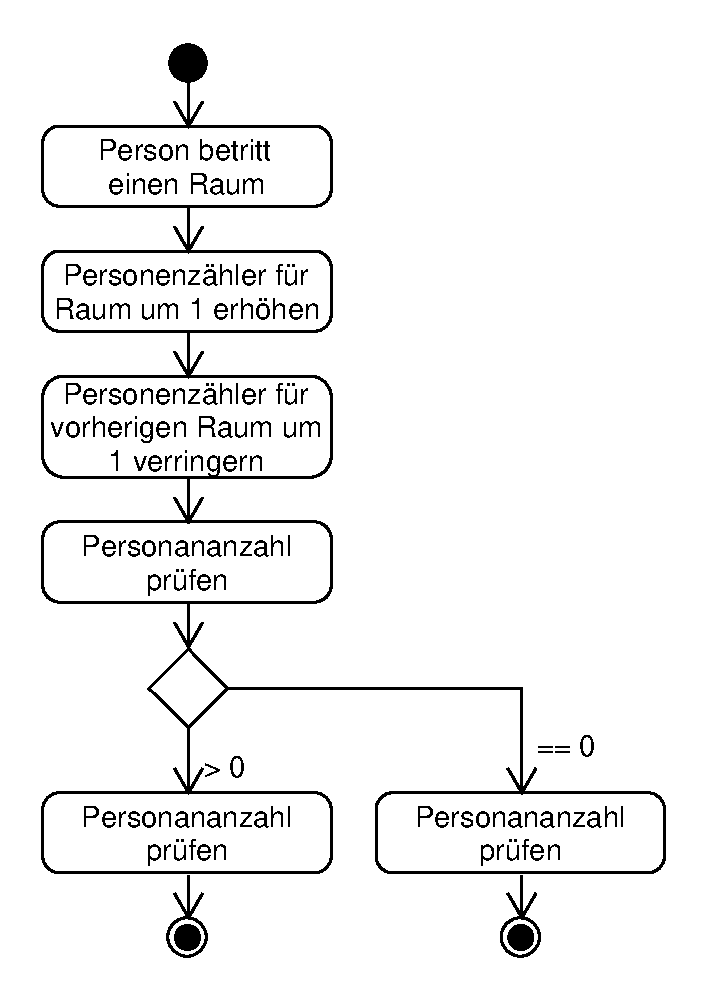
\includegraphics[scale=0.7]{img/Szenarien/ErkennungAnzahlPersonen.pdf}
	\caption{Erkennung der Personenanzahl}
	\label{fig:szenarienPersonenerkennung}
\end{figure}

\subsubsection{Modellierung Personenerkennung an der Tür}
\label{subsec:szenarioPersonTuer}
Das Modell (\prettyref{fig:szenarienPersonenerkennungTür}) zeigt den Ablauf für die beiden Bewegungssensoren an einem Türdurchgang. Dabei wird nach einer Aktivierung eines Sensors, auf einer Seite der Tür, auf den zweiten Sensor, auf der anderen Seite der Tür, eine gewisse Zeit gewartet. Sofern beide Sensoren innerhalb dieses gewissen Zeitraums aktiviert wurden, ist ein Durchgang erkannt worden und die jeweiligen Personenzähler der anliegenden Räume werden angepasst.

\begin{figure}[h!]
	\centering
	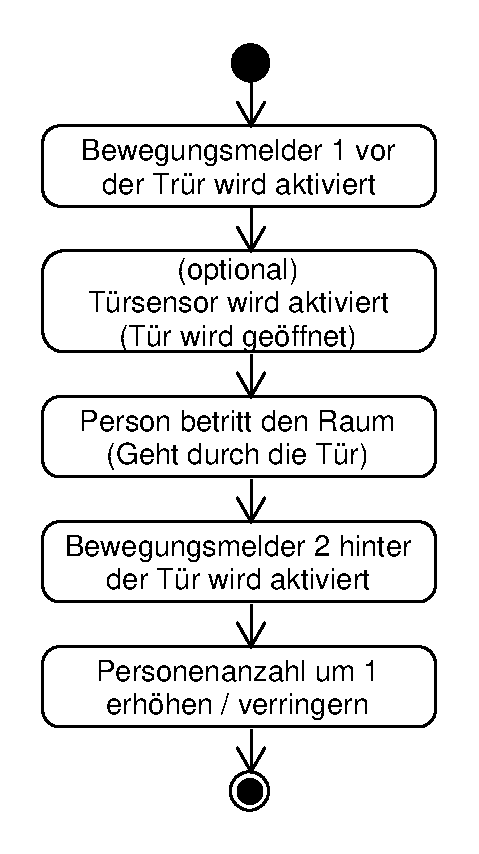
\includegraphics[scale=0.7]{img/Szenarien/PersonenerkennungAnTuer.pdf}
	\caption{Personenerkennung an der Tür}
	\label{fig:szenarienPersonenerkennungTür}
\end{figure}

\subsection{Haus bei verschließen der Haus-/ Wohnungstür in "`Standby"' versetzen}
\label{subsec:szenarioStandby}
\emph{(von Simon Schwabe)}
\subsubsection{Ablauf}
Um den Komfort in ihrem Smart Home zu steigern, möchte Anne möglichst wenig Aufwand zur Steuerung des Lichts betreiben. Dazu möchte sie bei Verlassen der Wohnung nicht alle angeschalteten Lampen manuell ausschalten und überprüfen, ob Gefahrenquellen vom Stromnetz getrennt sind.

Ein intelligentes, vernetztes Türschloss überträgt dazu beim Abschließen der Wohnung ein entsprechendes Signal an die zentrale Steuereinheit. Diese Steuereinheit interpretiert das Signal und schaltet alle Lampen aus. Außerdem werden vorher konfigurierte Steckdosen deaktiviert, um das Brandrisiko zu minimieren. Damit wird die Wohnung in einen "`Standby-Modus"' versetzt. Auch in diesem Fall möchte Anne nicht alle Geräte vom Stromnetz trennen, ihr Laptop soll weiterhin mit Strom versorgt und der Akku geladen werden.

Befindet sich Tom noch in der Wohnung, wenn sie abschließt, soll er nicht durch die Steuerung gestört werden. Das heißt in diesem Fall wird die automatische Abschaltung nicht durchgeführt. Dazu ist es notwendig, dass verschiedene Sensoren des Systems zuverlässig erkennen, ob Personen anwesend sind. Die automatische Steuerung wird erst aktiv, wenn der letzte Bewohner die Wohnung verlässt und abschließt.

Der Standby-Modus wird mit Aufschließen der Wohnungstür deaktiviert. Es erscheint allerdings nicht sinnvoll, den Zustand zum Zeitpunkt des Verlassens wiederherzustellen, da die Anforderungen an Beleuchtung usw. beim Ankommen grundlegend andere als bei Verlassen der Wohnung sein können. Diese sind abhängig von der Tageszeit.

\subsubsection{zur Diskussion}
\begin{itemize}
	\item welche Komponenten sind von der Abschaltung betroffen (z.B. Lampen, Steckdosen von Wasserkocher, Kaffeemaschine, ...)
	\item welche Komponenten sind ausgeschlossen (z.B. Kühl- und Gefrierschränke, Waschmaschinen, ...)
\end{itemize}

\subsubsection{erforderliche Komponenten}
\begin{itemize}
	\item Steuereinheit
	\item vernetztes Türschloss
	\item Sensoren zur Personenerkennung: z.B. Bewegungsmelder, Infrarot
	\item schaltbare Steckdosen, evtl. mit Verbrauchserkennung
	\item schaltbare Lampen
\end{itemize}


\subsubsection{Modellierung aus Nutzersicht}
Das Modell (\prettyref{fig:szenarienStandbyNutzersicht}) verdeutlicht die im Szenario beschriebene Interaktion des Nutzers mit dem System. Ziel des Szenarios ist es, dem Nutzer möglichst hohen Komfort zu bieten. Aus diesem Grund sind die Interaktionsmöglichkeiten des Nutzers mit dem System bewusst auf das Notwendigste beschränkt. Das Szenario wird indirekt durch den Nutzer initiiert, indem er die Wohnungstür abschließt. Auf diese Weise entsteht für die Nutzer kein Mehraufwand und keine direkte Interaktion mit dem System.

Mit dem Abschließen der Tür ist die Erwartung des Nutzers verbunden, dass die Wohnung in einen Standby-Modus tritt. Sollte dies aufgrund anwesender Personen nicht möglich sein, sollte der Nutzer über ein geeignetes Mittel darüber informiert werden. Dazu kann beispielsweise eine Benachrichtigung auf das Mobiltelefon des Nutzers gesendet werden.

\begin{figure}[h!]
	\centering
	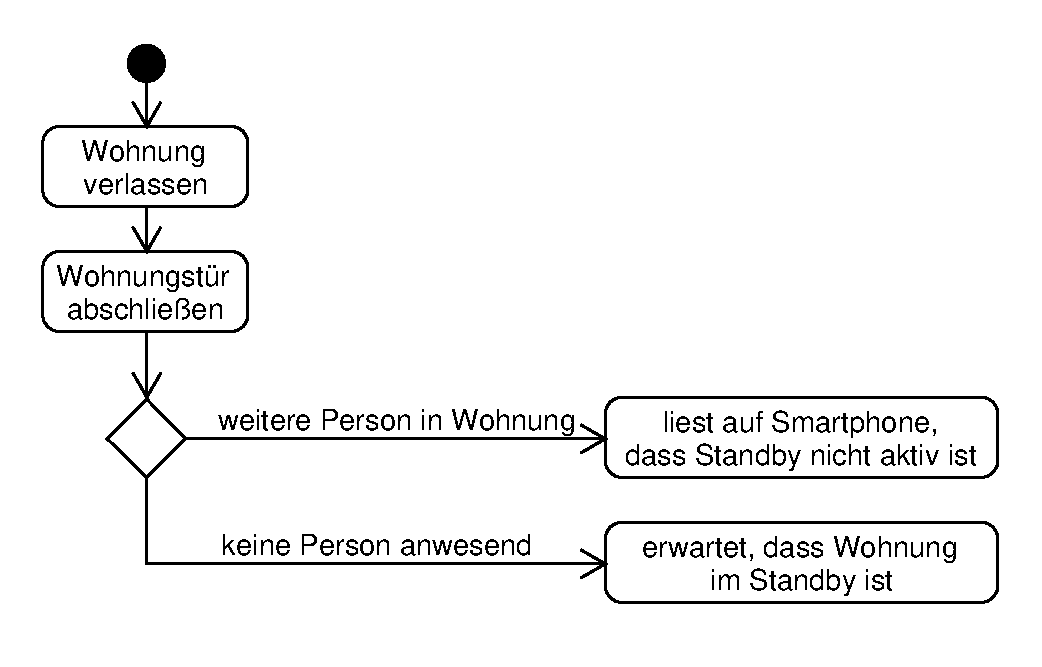
\includegraphics[scale=0.7]{img/Szenarien/WohnungSchliessenNutzersicht.pdf}
	\caption{Abläufe bei Verschließen der Wohnung aus Nutzersicht}
	\label{fig:szenarienStandbyNutzersicht}
\end{figure}

\subsubsection{Modellierung aus Systemsicht}
Die technische Modellierung (\prettyref{fig:szenarienStandby}) gestaltet sich etwas umfangreicher. Gestartet wird der Ablauf durch das Schließen des konfigurierten Schlosses. Alternativ kann auch ein Schalter an der Wohnungstür betätigt werden. Das System überprüft daraufhin, ob noch Personen in der Wohnung anwesend sind. Ist das der Fall, wird die Aktion abgebrochen und anwesende Personen werden nicht in ihren Aktivitäten beeinträchtigt. In diesem Fall kann der Nutzer, welcher die Wohnung verlassen hat, informiert werden.

Wird zum Zeitpunkt des Abschließens keine anwesende Person erkannt, wird ein Timer gestartet. So lange dieser Timer aktiv ist, wird in regelmäßigen Abständen überprüft, ob Personen, bzw. Bewegungen in der Wohnung erkannt werden. Dieses Vorgehen soll die Gefahr reduzieren, dass anwesende Personen nicht wahrgenommen werden. Wird während der Laufzeit des Timers eine Person erkannt, wird die Aktion wie oben beschrieben abgebrochen.

Trotz dieses Vorgehens ist nicht auszuschließen, dass Personen in der Wohnung nicht korrekt erkannt werden. Für diesen Fall kann ein zusätzlicher Feedback-Modus implementiert werden, in dem die anwesenden, nicht erkannten Personen über die anstehende Aktion informiert werden. Erfolgt kein Feedback, werden konfigurierte Geräte in den Standby-Modus versetzt.

\begin{figure}[h!]
	\centering
	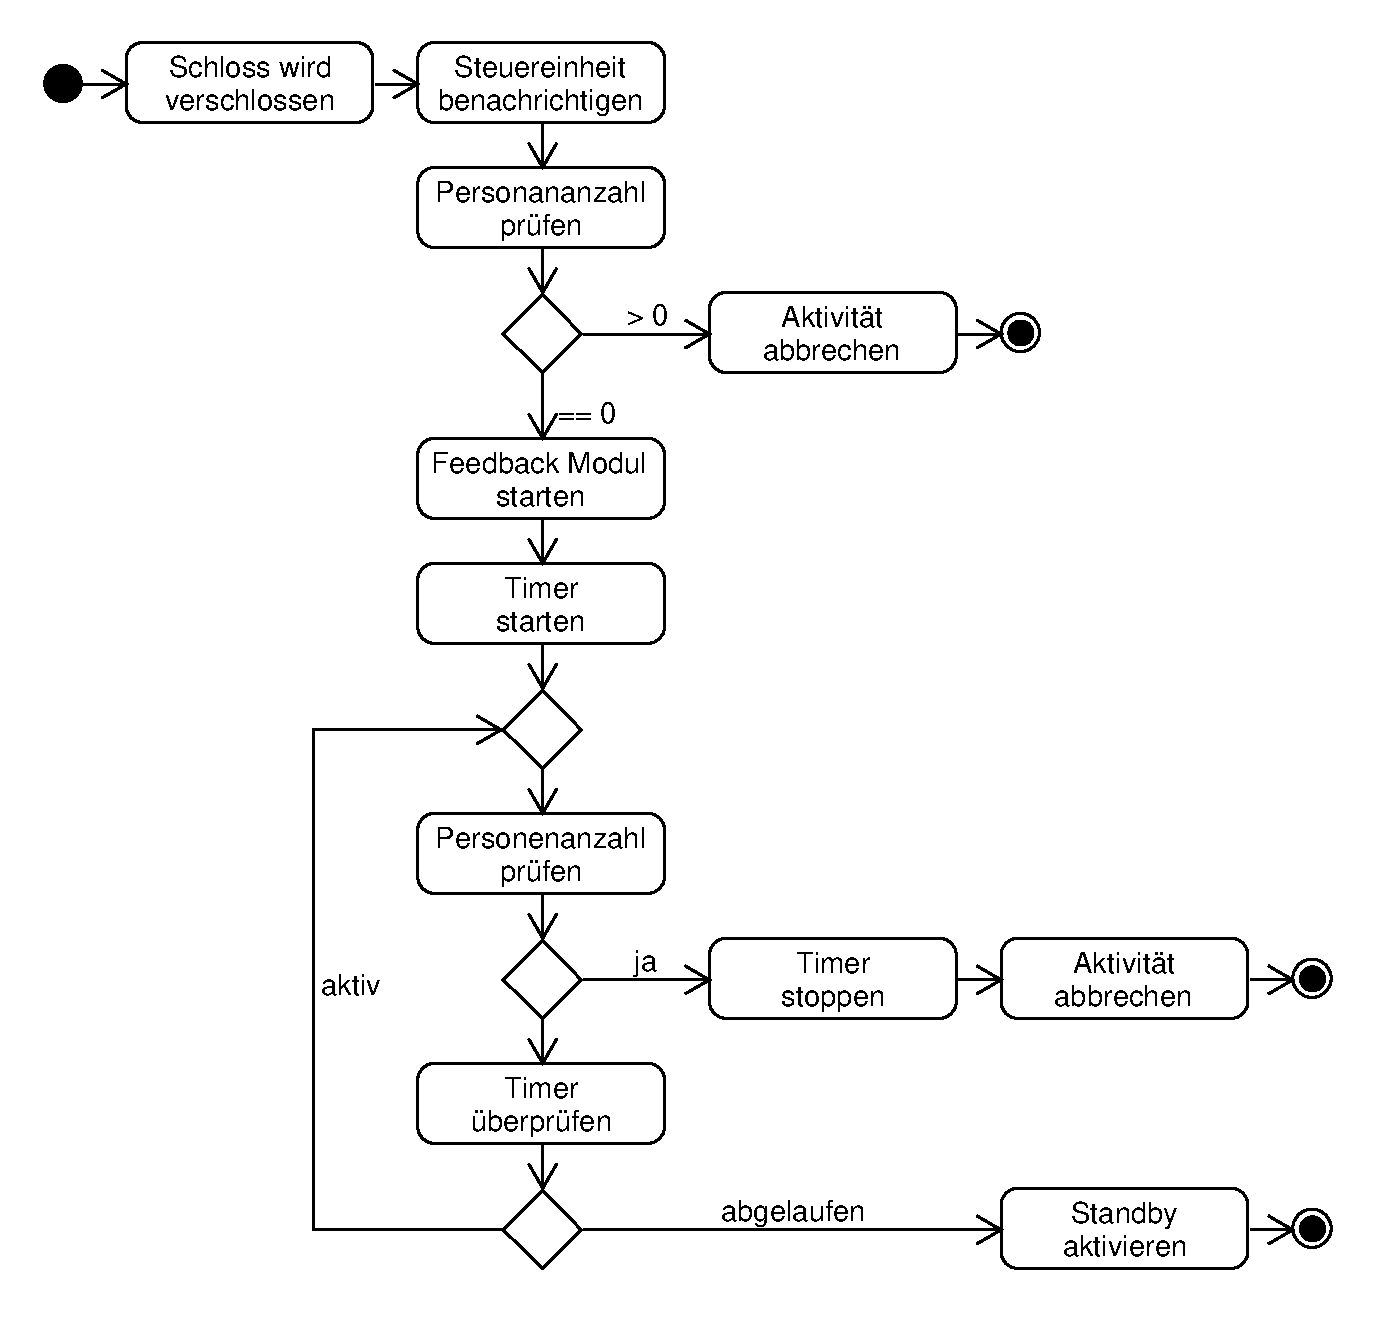
\includegraphics[width=0.9\textwidth]{img/Szenarien/WohnungSchliessen.pdf}
	\caption{Abläufe bei Verschließen der Wohnung aus Systemsicht}
	\label{fig:szenarienStandby}
\end{figure}

\subsection{Gefahrenquellen abstellen (Fibaro, CO$_2$)}
\emph{(von Martin Petzold)}
\subsubsection{Auslöser (opt.)}
\begin{itemize}
	\item Erkennung Erwachsene Person (Fibaro, CO$_2$)
\end{itemize}

\subsubsection{Vorbedingung}
\begin{itemize}
	\item Zuverlässige Erkennung ob Personen den Raum betreten oder verlassen (\prettyref{subsec:szenarioPersonTuer})
\end{itemize}

\subsubsection{Ablauf}
Das System befindet sich im Standby, d.h. alle Gefahrenquellen im Raum sind ausgeschaltet. Person X (ein Kind) betritt den Raum. Das Betreten des Raumes wird vom System erkannt und es wird ein Vorgang gestartet, der die Person als Kind oder Erwachsenen identifiziert. Person X wird dabei als Kind identifiziert und die Gefahrenquellen bleiben somit abgeschaltet. 
Nun betritt Person Y (ein Erwachsener) den Raum, dessen Betreten wird ebenfalls vom System erkannt. Der Erkennungsvorgang wird ein zweites Mal gestartet. Das System erkennt, dass es sich bei einer der beiden Personen um eine erwachsene Person handelt und schaltet die Gefahrenquellen frei, so dass diese benutzt werden können.
Nach einer Weile verlässt Person Y den Raum. Das System stellt fest das sich kein Erwachsener mehr im Raum befindet und schaltet nach einer gewissen Zeit den Standby Modus wieder her.

\subsubsection{Alternativer Ablauf}
Nur Person Y (ein Erwachsener) betritt den Raum und das System erkennt den Eintritt. Er wird beim Identifizierungsvorgang als Erwachsener erkannt und damit werden die Gefahrenquellen freigeschaltet.
Nach einer Weile verlässt Person Y den Raum. Das System stellt fest das sich kein Erwachsener mehr im Raum befindet und schaltet nach einer gewissen Zeit den Standby Modus wieder her.

\subsubsection{erforderliche Komponenten}
\begin{itemize}
	\item Fibaro 6 in 1 Sensor
	\item CO$_2$ Sensor
	\item Z-Way-Server/Steuereinheit
	\item 2 Bewegungsmelder zur Erkennung von Eintritt in den Raum
	\item Schaltbare Gefahrenquelle oder zur Simulation eine schaltbare Lampe
\end{itemize}

\subsubsection{Nachbedingung}
\begin{itemize}
	\item Das System kann auch eine Regelung beinhalten, dass der Standby Modus automatisch und nicht nach verlassen des Raumes zeitgesteuert wieder hergestellt wird.
\end{itemize}

\subsubsection{zur Diskussion}
\begin{itemize}
	\item Abgleich mit dem Szenario zur Erkennung ob eine Person den Raum betreten/verlassen hat
	\item sind die Sensoren präzise genug um den Unterschied zwischen Kind und Erwachsener zu erfassen, oder kann nur Mensch und Haustier unterschieden werden
	\item soll die Reaktivierung des Standby Modus Teil des Szenarios sein
	\item Einordnung in umsetzbar/nicht umsetzbar
\end{itemize}

\subsubsection{ähnliche Szenarien}
\begin{itemize}
	\item \prettyref{subsec:szenarioPersonTuer}
	\item \prettyref{subsec:szenarioStandby}
\end{itemize}

\subsubsection{Modellierung Identifizierung Erwachsener}
\emph(//TODO BITTE NOCH BESCHREIBUNGSTEXT EINFÜGEN (siehe Modell)) bereits gemacht?

Wenn sich die Personenanzahl eines Raumes ändert wird unterschieden, ob die Person den Raum betreten oder verlassen hat. Danach wird die Größenmessung und CO$_2$ Messung gestartet. Wenn eine Person den Raum betreten hat, wird die Größenerkennung abgeglichen und anhand des Ergebnisses die Anzahl der Erwachsenen erhöht. Verlässt eine Person den Raum, dann wird der Counter verringert. Wenn der erwachsenenCounter Geringer als 1 ist oder die CO$_2$ Messung keinen Erwachsenen erkennt wird der Vorgang mit kein Erwachsener vorhanden beendet. Nur wenn sowohl die Größenmessung und die CO$_2$ Messung einen Erwachsenen erkennen, wird "`Erwachsener erkannt"' ausgegeben.
\begin{figure}[h!]
	\centering
	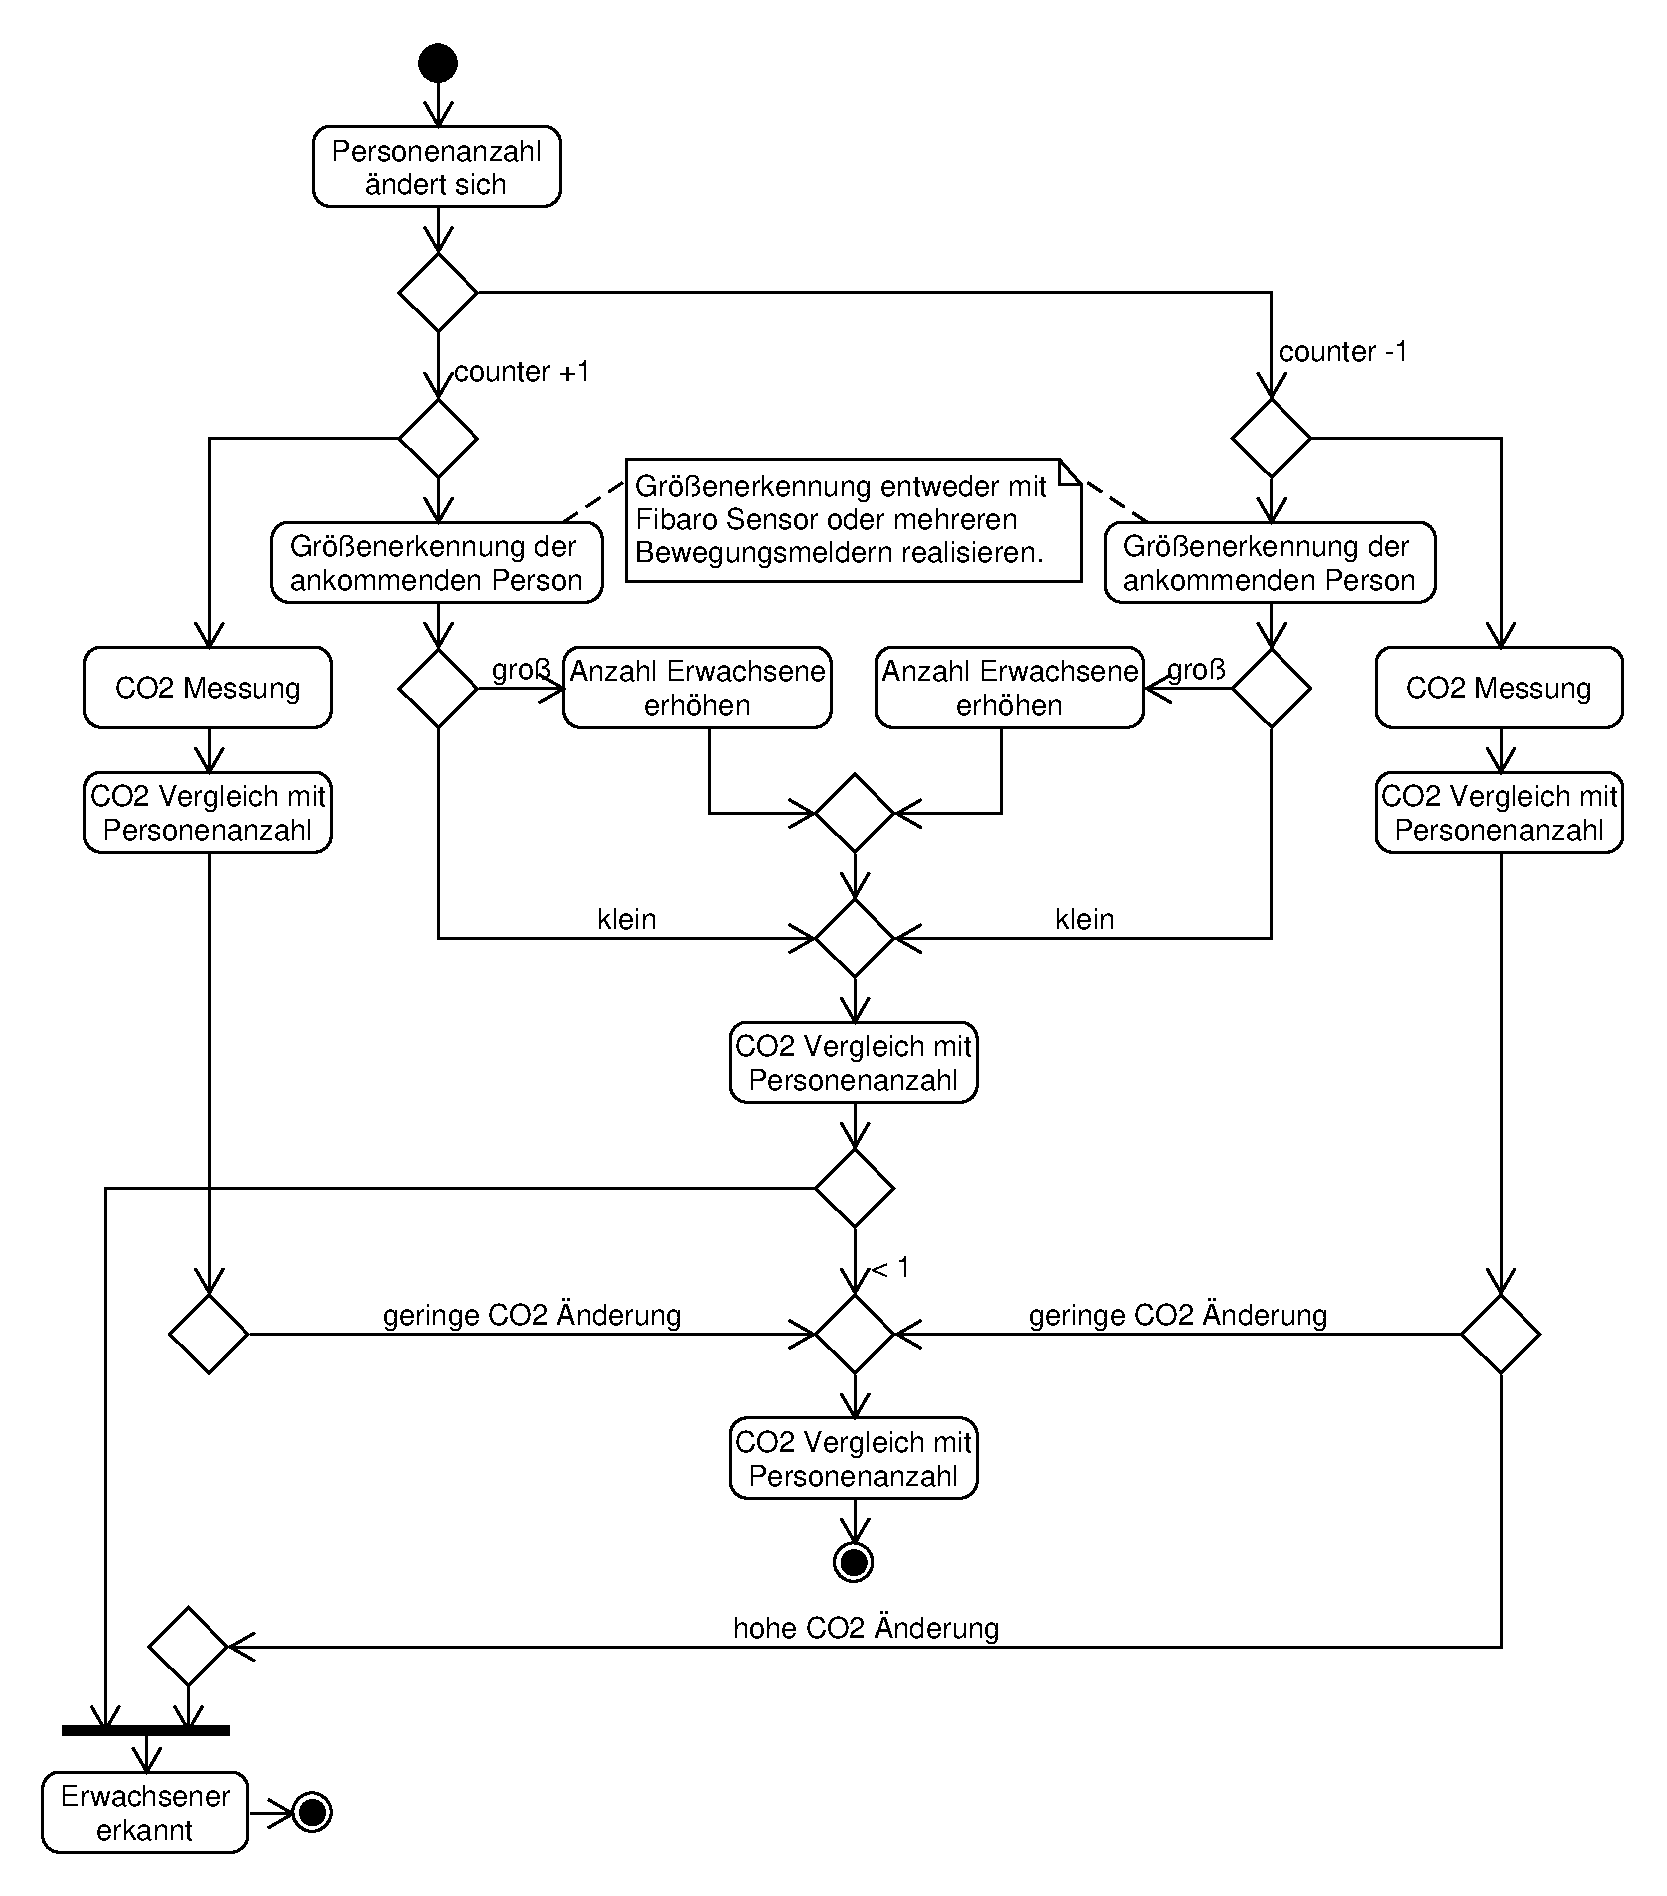
\includegraphics[width=0.9\textwidth]{img/Szenarien/IdentifizierungErwachsene.pdf}
	\caption{Identifizierung Erwachsener}
	\label{fig:szenarienIdentifizierungErwachsene}
\end{figure}

\subsubsection{Modellierung Gefahrenquellen abstellen}
\emph(//TODO BITTE NOCH BESCHREIBUNGSTEXT EINFÜGEN (siehe Modell)) bereits gemacht?

Wenn sich die Personenanzahl eines PersonCounters ändert, wird die Identifizierung gestartet, ob sich ein Erwachsener im Raum befindet. Wird ein Erwachsener erkannt wird der Zustand der Gefahrenquellen ausgelesen und, wenn nötig, freigeschaltet. Wird bei der Identifizierung kein Erwachsener erkannt wird ebenfalls der Zustand der Gefahrenquellen ausgelesen und gegebenenfalls ein Timer zu deren Abschaltung gestartet, welcher bei erneuter Änderung der Personenanzahl gestoppt wird.

\begin{figure}[h!]
	\centering
	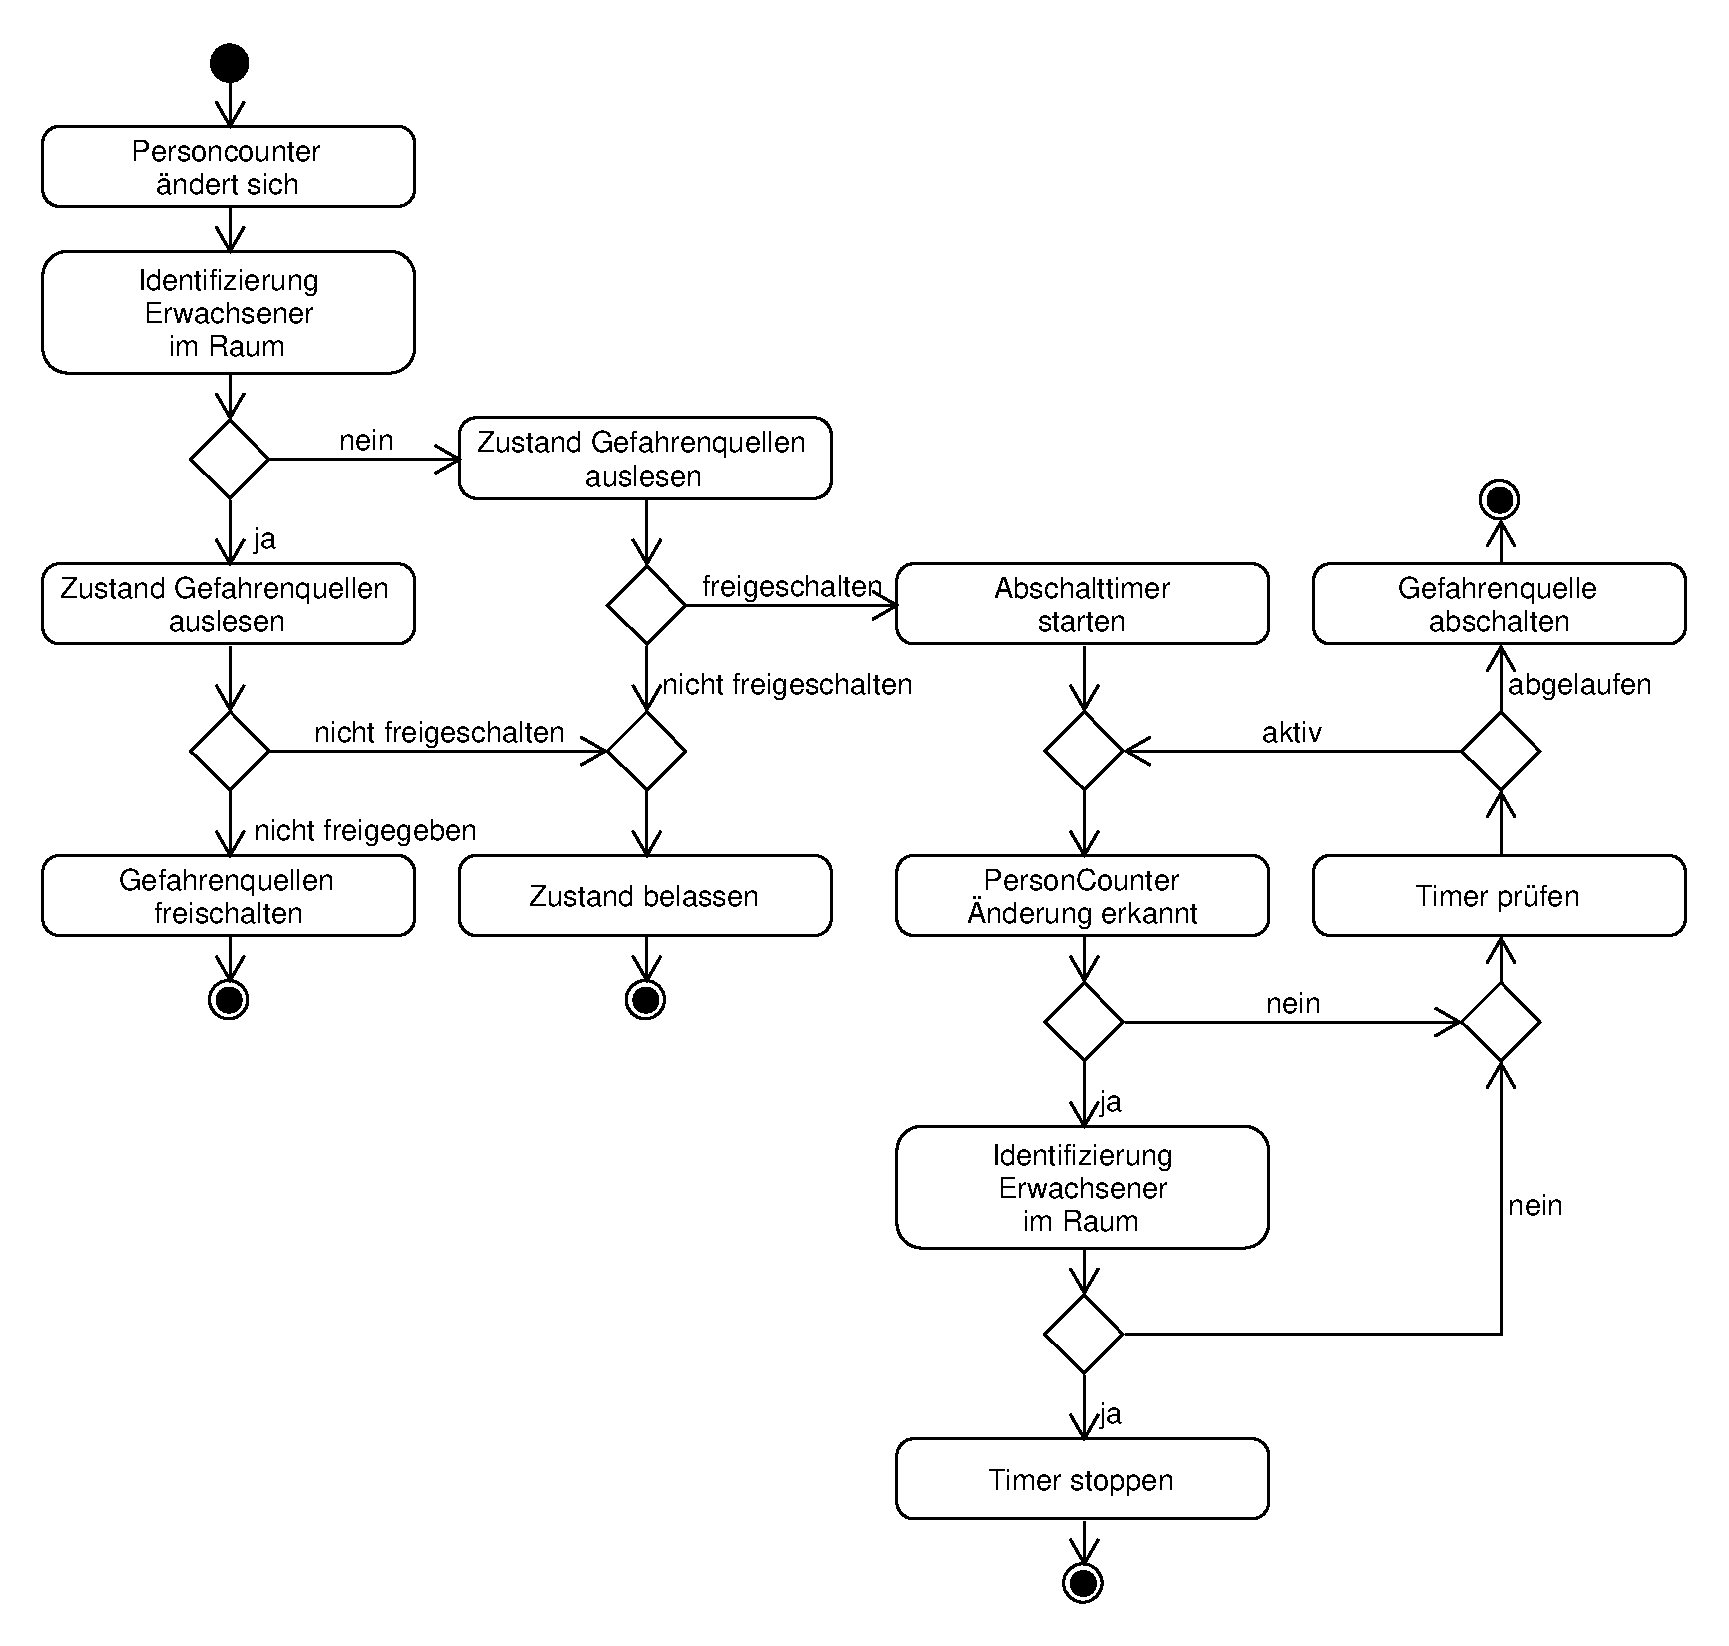
\includegraphics[width=0.9\textwidth]{img/Szenarien/GefahrenquellenAbstellen.pdf}
	\caption{Gefahrenquellen abstellen}
	\label{fig:szenarienGefahrenquellenAbstellen}
\end{figure}


\section{Modulkonzeption}
TODO: allgemeine Beschreibung aller Module, deren Zusammenwirken (Grafik).

\subsection{LockDoorModule}
\emph{(von Simon Schwabe)}

\subsubsection{Allgemein}
Das LockDoor-Modul ist der Vermittler für weitere Module im Zusammenhang mit dem Verlassen der Wohnung. Wenn die Wohnung verlassen und abgeschlossen wird, ist die Wahrscheinlichkeit hoch, dass keine weiteren Personen anwesend sind. Allerdings kann die Wohnung auch irrtümlich abgeschlossen werden und es sind noch weitere Personen anwesend. Um solchen Fehlinterpretationen entgegenzuwirken überprüft das LockDoor-Modul immer, ob wirklich keine Personen erkannt werden und die Wohnung leer steht. Diese Information ist für weitere Module, insbesondere das Alarm-Modul, relevant und wird über den Event Bus mitgeteilt.

\subsubsection{Funktionsweise}
Die genaue Funktionsweise des Moduls wurde im Wesentlichen schon im Abschnitt Szenarien (siehe \prettyref{subsec:szenarioStandby}) beschrieben und modelliert. Das Modell „Abläufe bei Verschließen der Wohnung aus Systemsicht“ (\prettyref{fig:szenarienStandby}) beschreibt das Vorgehen. Die Aktivität „Standby aktivieren“ kann um das Werfen des entsprechenden Events erweitert werden.

Das Szenario enthält keine detaillierte Beschreibung für die Abschaltung des Standby-Modus, da dies nicht notwendig ist. Für das LockDoor-Modul ist es allerdings erforderlich auf die Ankunft von Personen zu reagieren, z.B. um das Alarm-Modul zu benachrichtigen und die Alarmanlage abzuschalten. %Die Anzahl der durchzuführenden Aktionen ist überschaubar und wird im Modell dargestellt (\prettyref{fig:modulkonzeptionLockDoorSequence}).
Dazu wird bei Ankunft der entsprechende Schalter betätigt, bzw. das Schloss geschlossen. Anschließend wird das Event "`LockDoorModule\_unlocked"' geworfen. An dieser Stelle ist keine weitere Logik erforderlich.

%TODO Grafik an geeigneter Stelle einbinden und beschreiben.
\begin{figure}[h!]
	\centering
	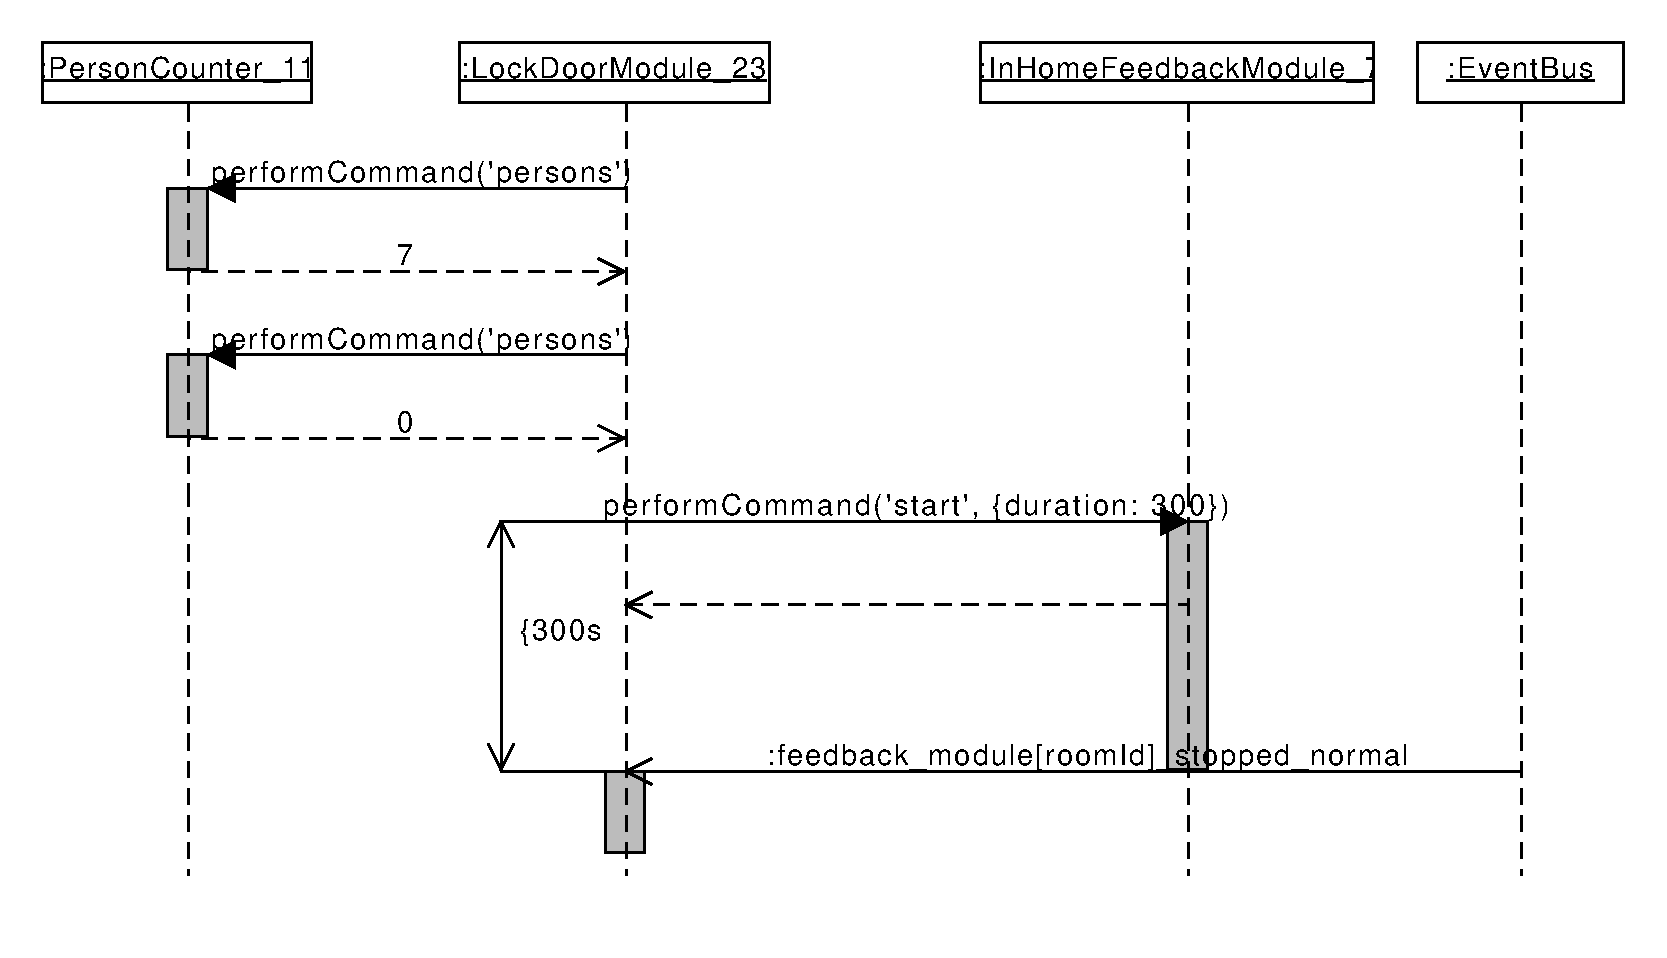
\includegraphics[width=0.9\textwidth]{img/Modulkonzeption/LockDoorSequence.pdf}
	\caption{Sequenzdiagramm - LockDoor-Modul}
	\label{fig:modulkonzeptionLockDoorSequence}
\end{figure}

\subsubsection{Konfiguration}
Bei der Konfiguration des LockDoor-Moduls muss das Wohnungstürschloss angegeben werden, alternativ kann dafür ein Schalter benutzt werden, der im Inneren der Wohnung vor dem Verlassen betätigt wird. 
\begin{itemize}
	\item Schloss/Schalter
	\begin{itemize}
		\item Typ: BinarySwitch
		\item erforderlich: ja
	\end{itemize}
\end{itemize}

\subsubsection{Schnittstellen}
Die Schnittstellen, welche dieses Modul nutzt und bereitstellt, sind von großer Bedeutung. Das Modul an sich implementiert eine nur geringe Funktionalität, jedoch ist es eine Brücke zwischen den Modulen zur Raumüberwachung auf der einen Seite, und den Modulen für Aktionen beim Verlassen der Wohnung auf der anderen Seite.

Das LockDoor-Modul bietet über den Event Bus eine Schnittstelle zu anderen Modulen. Diese werden benachrichtigt, sobald davon ausgegangen wird, dass keine Person mehr anwesend ist (LockDoorModule\_locked). Die Freischaltung geschieht über ein weiteres Event (LockDoorModule\_unlocked).

Das Modul wird als Singleton angelegt, da für jede Wohnung nur ein Modul zur Überwachung der Wohnungstür erforderlich ist. Das hat zur Folge, dass Events keine Virtual Device Id tragen. Damit ist es für Empfänger einfacher, auf entsprechende Events zu reagieren.

Für die Überprüfung der Personenanzahl wird die Schnittstelle des Moduls PersonCounter genutzt. Dazu wird für jeden Raum die Anzahl der Personen überprüft.


%\begin{tabularx}{\textwidth}{ X X X }
%	\hline \multicolumn{3}{c}{\textbf{Event Bus - Senden}}  \\ 
%	\hline Event Name 					& Parameter 	& Beschreibung \\ 
%	\hline door\_lock\_module\_locked	& - 			& Tür verschlossen, keine Person anwesend \\ 
%	\hline door\_lock\_module\_unlocked & - 			& Tür geöffnet \\ 
%	\hline 
%\end{tabularx}

\begin{table}[h!]
\begin{tabularx}{\textwidth}{
		 >{\hsize=1.25\hsize}X % 40% of 3\hsize 
		>{\hsize=0.5\hsize\centering}X % 30% of 3\hsize
		>{\hsize=1.25\hsize}X % 40% of 3\hsize
		% sum=3.0\hsize for 3 columns
	}
	\hline
	\textbf{Event Name}					& \textbf{Parameter}	& \textbf{Beschreibung} \\
	\hline LockDoorModule\_locked		& - 					& Tür verschlossen, keine Person anwesend \\ 
	\hline LockDoorModule\_unlocked		& - 			 		& Tür geöffnet \\ 
	\hline
\end{tabularx}
\caption{LockDoorModule: Schnittstelle Event Bus}
\end{table}


%\begin{longtable}{R{5cm} L{7cm}}
%	\toprule
%	\textit{Option} & \textit{Konfiguration} \\
%	\midrule
%	Feedbackart & Frage \\ [0.25cm]
%	Feedback von & Nutzer mit E-Mail-Adresse für Rückmeldungen \\[0.25cm]
%	Ausführender & Mitarbeiter der Abteilung \glqq Qualitätssicherung\grqq \\[0.25cm]
%	Kategorie & Einordnung in die Kategorie \glqq Mobiles Menü-Bestellsystem\grqq \\[0.25cm]
%	Erklärung & Frage mit Zusatzinformationen zur Menükomponente auf die sich die Frage bezieht \\[0.25cm]
%	\bottomrule	
%	\caption{Beispielkonfiguration des CRM Systems}
%\end{longtable}

\subsubsection{Abhängigkeiten}
\begin{itemize}
	\item PersonCounterModule
	\item TurnOffTimerModule
\end{itemize}
Das PersonCounter-Modul wird zur Überprüfung der Personenanzahl je Raum genutzt. Dazu werden Aufrufe über die ZAutomation-API an das Modul gesendet.

Das TurnOffTimer-Modul stellt eine Schnittstelle zum Feedback-Modul her. Durch die zusätzliche Abstraktionsschicht des TurnOffTimer-Moduls arbeitet das LockDoor-Modul nicht direkt gegen das Feedback-Modul, sondern startet lediglich den Timer. Dieser übernimmt die Kommunikation mit dem Feedback-Modul.

\subsubsection{Interne Speicher}
\begin{itemize}
	\item konfiguriertes Türschloss
\end{itemize}

\subsection{PersonCounterModule}
\emph{(von Philip Laube)}
\subsubsection{Allgemein}
Das PersonCounterModule übernimmt die Aufgabe, die Anzahl der Personen im jeweiligen Raum zu speichern. Jede Möglichkeit einer Erkennung ob eine Person den Raum betreten oder verlassen hat kann über dieses Modul kommuniziert werden um es anderen Modulen zur Verfügung zu stellen. Dies macht dieses Modul zu einem zentralen Bestandteil.

Ein PersonCounterModule enthält zusätzlich die Information, für welchen Raum es bestimmt ist. Somit kann es beliebig oft wiederverwendet werden.

Der jeweilige Personenzähler pro Raum wird durch Module, die ihn benötigen, instanziiert. Vorhandene Personenzähler werden einfach verwendet.

\subsubsection{Funktionsweise}
Dieses Modul wird nur indirekt benutzt. Es dient als Datenhaltung für die wichtige und von anderen Modulen benötige Informationen der Personenanzahl (\prettyref{fig:szenarienPersonenerkennung}).

Die Instanziierung des Moduls findet entweder zentral über ein Modul statt oder wird als Funktion bereitgestellt. Es kann dann entweder automatisch oder pro Modul über eine Funktion instanziiert und benutzt werden.

\subsubsection{Konfiguration}
\begin{itemize}
	\item Zähler
	\begin{itemize}
		\item Typ: Metrik
		\item Erforderlich: ja
	\end{itemize}
	\item Raum
	\begin{itemize}
		\item Typ: Text
		\item Erforderlich: ja
	\end{itemize}
\end{itemize}

\subsubsection{Schnittstellen}

\begin{table}[H]
	\begin{tabularx}{\textwidth}{
			>{\hsize=1.25\hsize}X % 40% of 3\hsize 
			>{\hsize=0.5\hsize\centering}X % 30% of 3\hsize
			>{\hsize=1.25\hsize}X % 40% of 3\hsize
			% sum=3.0\hsize for 3 columns
		}
		\hline
		\textbf{URL}						& \textbf{Parameter}	& \textbf{Beschreibung} \\
		\hline /command/person\_entered		& - 					& Erhöht den Zähler um 1. \\ 
		\hline /command/person\_left		& - 			 		& Mindert den Zähler um 1. \\
		\hline /command/persons				& - 					& Liefert die aktuelle Anzahl an Personen des Raums. \\
		\hline
	\end{tabularx}
	\caption{PersonCounterModule: Schnittstelle ZAutomation}
\end{table}

\begin{table}[H]
	\begin{tabularx}{\textwidth}{
			>{\hsize=1.5\hsize}X 
			>{\hsize=0.5\hsize}X
		}
		\hline
		\textbf{Event Name}													& \textbf{Beschreibung} \\
		\hline [DeviceId]:PersonCounterModule\_[RaumId]\_person\_entered	& - \\ 
		\hline [DeviceId]:PersonCounterModule\_[RaumId]\_person\_left		& - \\
		\hline
	\end{tabularx}
	\caption{PersonCounterModule: Schnittstelle Event Bus}
\end{table}

\subsubsection{Abhängigkeiten}
\begin{itemize}
	\item Keine, da dieses Modul Grundfunktionalitäten bereitstellt.
\end{itemize}

\subsubsection{Interne Speicher}
\begin{itemize}
	\item Raum ID
	\item Anzahl der Personen im Raum
\end{itemize}


\subsection{RoomAccessModule}
\emph{(von Philip Laube)}

\subsubsection{Allgemein}
Das RoomAccessModule übernimmt die Aufgabe, Personen zu erkennen, die einen Raum verlassen oder betreten haben. Dies geschieht entweder unverzüglich oder zeitversetzt, je nach Art der zugrundeliegende Module.

Dieses Modul stellt grundlegende Unterstützung zunächst für Bewegungssensoren, später eventuell auch erweiterte Logik für andere Sensoren zur Personenerkennung bzw. Raumwechsel.

Ein RoomAccessModule enthält zusätzlich die Information für welche Räume es bestimmt ist, somit kann es beliebig oft wiederverwendet werden.

\subsubsection{Funktionsweise}
Diese Realisierung entspricht der geplanten Realisierung des Szenarios zu Beginn des Projekts (\prettyref{subsec:szenarioPersonCounter}). Exakt diese Logik wird zunächst durch dieses Modul implementiert (\prettyref{fig:szenarienPersonenerkennungTür}).

Es wird der zugehörige Personenzähler der jeweiligen Räume angesprochen und die Anzahl jeweils korrigiert. Weitere Logik anderer Module kann durch ein Event erfolgen. Jedwede Logik die direkt mit der Personenanzahl in Verbindung steht muss den Personenzähler (PersonCounterModule) ansprechen.

\subsubsection{Konfiguration}
\begin{itemize}
	\item Sensor Eins
	\begin{itemize}
		\item Typ: Bewegungssensor
		\item Erforderlich: ja
	\end{itemize}
	
	\item Raum Eins
	\begin{itemize}
		\item Typ: Raum
		\item Erforderlich: ja
	\end{itemize}

	\item Sensor Zwei
	\begin{itemize}
		\item Typ: Bewegungssensor
		\item Erforderlich: ja
	\end{itemize}
	
	\item Raum Zwei
	\begin{itemize}
		\item Typ: Raum
		\item Erforderlich: ja
	\end{itemize}

\end{itemize}

\subsubsection{Schnittstellen}
\begin{table}[H]
	\begin{tabularx}{\textwidth}{
			>{\hsize=1.25\hsize}X 
			>{\hsize=0.75\hsize}X
			% sum=2.0\hsize for 2 columns
		}
		\hline
		\textbf{Event Name}						& \textbf{Beschreibung} \\
		\hline [DeviceId]:RoomAccessModule\_[verlassenderRaumId]\_[betretenerRaumId]\_transition\_detected	& Wenn ein Übergang einer Person von einem Raum in den nächsten 	Raum erfolgt ist wird dieses Event ausgelöst \\ 
		\hline 
	\end{tabularx}
	\caption{RoomAccessModule: Schnittstellen Event Bus}
\end{table}

\subsubsection{Abhängigkeiten}
\begin{itemize}
	\item Daten des PersonCounterModule zum Zählen der Personen in einem Raum
\end{itemize}

\subsubsection{Interne Speicher}
\begin{itemize}
	\item zwei Bewegungssensoren
	\item Raum Zuordnung der beiden Sensoren
	\item PersonenCounterModule der Raumzuordnungen
\end{itemize}

\subsection{StandbyModule}
\emph{(von Zarina Muratbekovna Omurova)}
\subsubsection{Allgemein}
Das StandbyModule übernimmt die Aufgabe, das Haus in einen Standby-Modus zu versetzen.

Im Fall, dass niemand zu Hause ist und das Event "`LockDoor\_locked"' vom LockDoorModule eingegangen ist, werden ausgewählte Geräte, wie Lampen, Heizung oder Elektrogeräte im Haus in einen definierten Zustand geschaltet. Manche Geräte, z.B. Steckdosen, sollen ausgeschaltet werden, wenn die Wohnung in den Standby-Modus geht. Andere Geräte, z.B. Orientierungsleuchten oder Alarmanlagen sollen angeschaltet werden. Diese Geräte und die entsprechenden Aktionen werden beim Anlegen des StandbyModules konfiguriert.

Bei dem Event "`LockDoor\_unlocked"', werden keine Aktionen durchgeführt, dies bewirkt, dass der interne Zustand des StandbyModules auf "`stopped"' geändert wird.

Wenn die Tür geöffnet wird, wird automatisch der Standby-Modus ausgeschaltet und ein entsprechendes Event an andere Module gesendet.

\subsubsection{Funktionsweise}

\begin{figure}[h!]
	\centering
	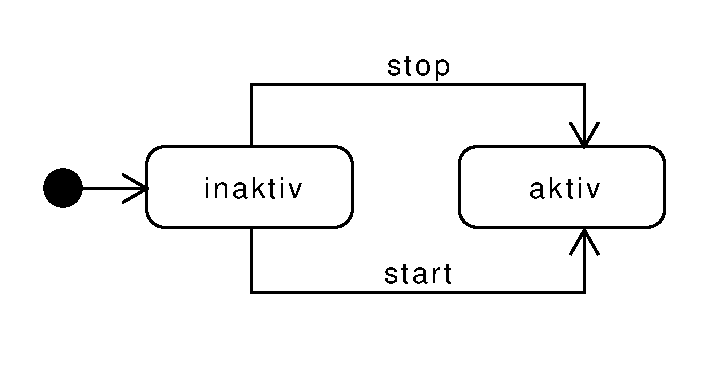
\includegraphics[scale=0.7]{img/Modulkonzeption/StandbyStateMachine.pdf}
	\caption{Zustandsdiagramm – StandbyModule}
	\label{fig:standbyStateMachine}
\end{figure}


Dieses Modell veranschaulicht die verschiedenen internen Zustände des StandbyModules und deren Zustandsübergänge. Wenn es im inaktiven Zustand ist, wird das Modul durch einen Startkommando in einen aktiven Zustand übergehen und im aktivem Zustand kann das Modul in einen inaktiven Zustand wechseln.

\subsubsection{Konfiguration}
\begin{itemize}
	\item Geräte, welche bei Aktivierung des Standby geschaltet werden
	\begin{itemize}
		\item 	Typ: Liste [Switch Binary, Switch Multilevel]
		\item Aktion: on/off 
		\item Erforderlich: ja
	\end{itemize}
	\item Geräte, welche bei Dektivierung des Standby geschaltet werden
	\begin{itemize}
		\item 	Typ: Liste [Switch Binary, Switch Multilevel]
		\item Aktion: on/off 
		\item Erforderlich: ja
	\end{itemize}
	\item Raum
	\begin{itemize}
		\item Typ: Text
		\item Erforderlich: ja
	\end{itemize}
\end{itemize}

\subsubsection{Schnittstellen}
\begin{table}[H]
	\begin{tabularx}{\textwidth}{
			>{\hsize=1.25\hsize}X % 40% of 3\hsize 
			>{\hsize=0.5\hsize\centering}X % 30% of 3\hsize
			>{\hsize=1.25\hsize}X % 40% of 3\hsize
			% sum=3.0\hsize for 3 columns
		}
		\hline
		\textbf{URL}						& \textbf{Parameter}	& \textbf{Beschreibung} \\
		\hline /command/started				& - 					& Starten des Standby-Modus. \\ 
		\hline /command/stopped				& - 			 		& Stoppen des Standby-Modus. \\
		\hline /command/state				& stopped started	& Liefert den aktuellen Zustand des Moduls. \\
		\hline
	\end{tabularx}
	\caption{StandbyModule: Schnittstelle ZAutomation}
\end{table}

\begin{table}[H]
	\begin{tabularx}{\textwidth}{
			>{\hsize=1.25\hsize}X % 66.66% of 3\hsize 
			>{\hsize=0.5\hsize\centering}X % 16.66% of 3\hsize
			>{\hsize=1.25\hsize\centering\arraybackslash}X % 16.66% of 3\hsize
			% sum=3.0\hsize for 3 columns
		}
		\hline
		\textbf{Event Name}								& \textbf{Parameter}	& \textbf{Beschreibung} \\
		\hline [DeviceId]:StandbyModule\_[RaumId]\_started	& - 				& Standby-Modus wurde gestartet \\ 
		\hline [DeviceId]:StandbyModule\_[RaumId]\_stopped	& - 				& Standby-Modus wurde beendet \\
		\hline
	\end{tabularx}
	\caption{StandbyModule: Schnittstelle Event Bus}
\end{table}

\subsubsection{Abhängigkeiten}
\begin{itemize}
	\item Module Events (LockDoor)
\end{itemize}

\subsubsection{Interne Speicher}
\begin{itemize}
	\item Raum ID
	\item Zustand des Raums (im Standby: stopped/started)
	\item Switches/Dimmers
\end{itemize}

\subsection{InHomeFeedbackModule}
\emph{(von Patrick Hecker)}
\subsubsection{Allgemein}
Das Feedback-Modul übernimmt die Aufgabe, Personen im Haus über eingehende Aktionen zu informieren. Neben den eingehenden Aktionen (von Personen außerhalb des Hauses) kann auch auf Aktionen, die vom System automatisch gestartet wurden, hingewiesen werden (Timer, Grenzwert eines Sensors überschritten, ...). Die Personen im Haus haben dadurch die Möglichkeit auf Aktionen zu reagieren, indem sie sie abbrechen bzw. verzögern können. Der konkrete Feedbackmechanismus kann individuell konfiguriert werden und gliedert sich in folgende fünf Kategorien (detaillierter in Abschnitt Konfiguration).

\begin{itemize}
	\item visuelles Feedback (bspw. Lampen, LED’s an Schalter, ...),
	\item akustisches Feedback (bspw. Sirene, ...)
	\item Nachricht (bspw. E-Mail, Push-Nachricht, ...)
	\item Aufruf spezieller Module (bspw. Philips Hue, Bose, ...)
	\item HTTP
	\item JavaScript
\end{itemize}
Ein Feedbackmodul enthält zusätzlich die Information für welchen Raum es bestimmt ist, somit kann es beliebig oft wiederverwendet werden.

\subsubsection{Funktionsweise}

\begin{figure}[h!]
	\centering
	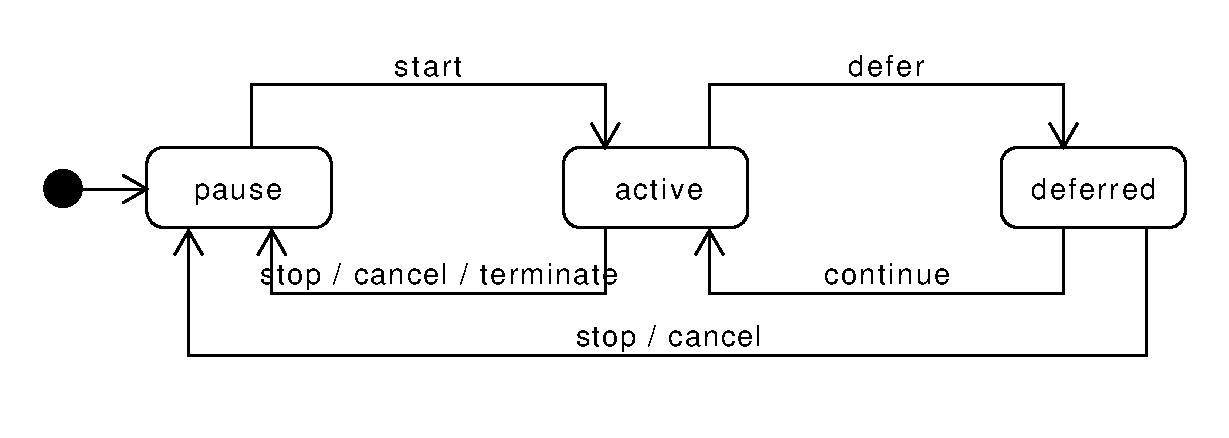
\includegraphics[scale=0.7]{img/Modulkonzeption/FeedbackStateMachine.pdf}
	\caption{Zustandsdiagramm – InHomeFeedback-Modul}
	\label{fig:feedbackStateMachine}
\end{figure}

\begin{figure}[h!]
	\centering
	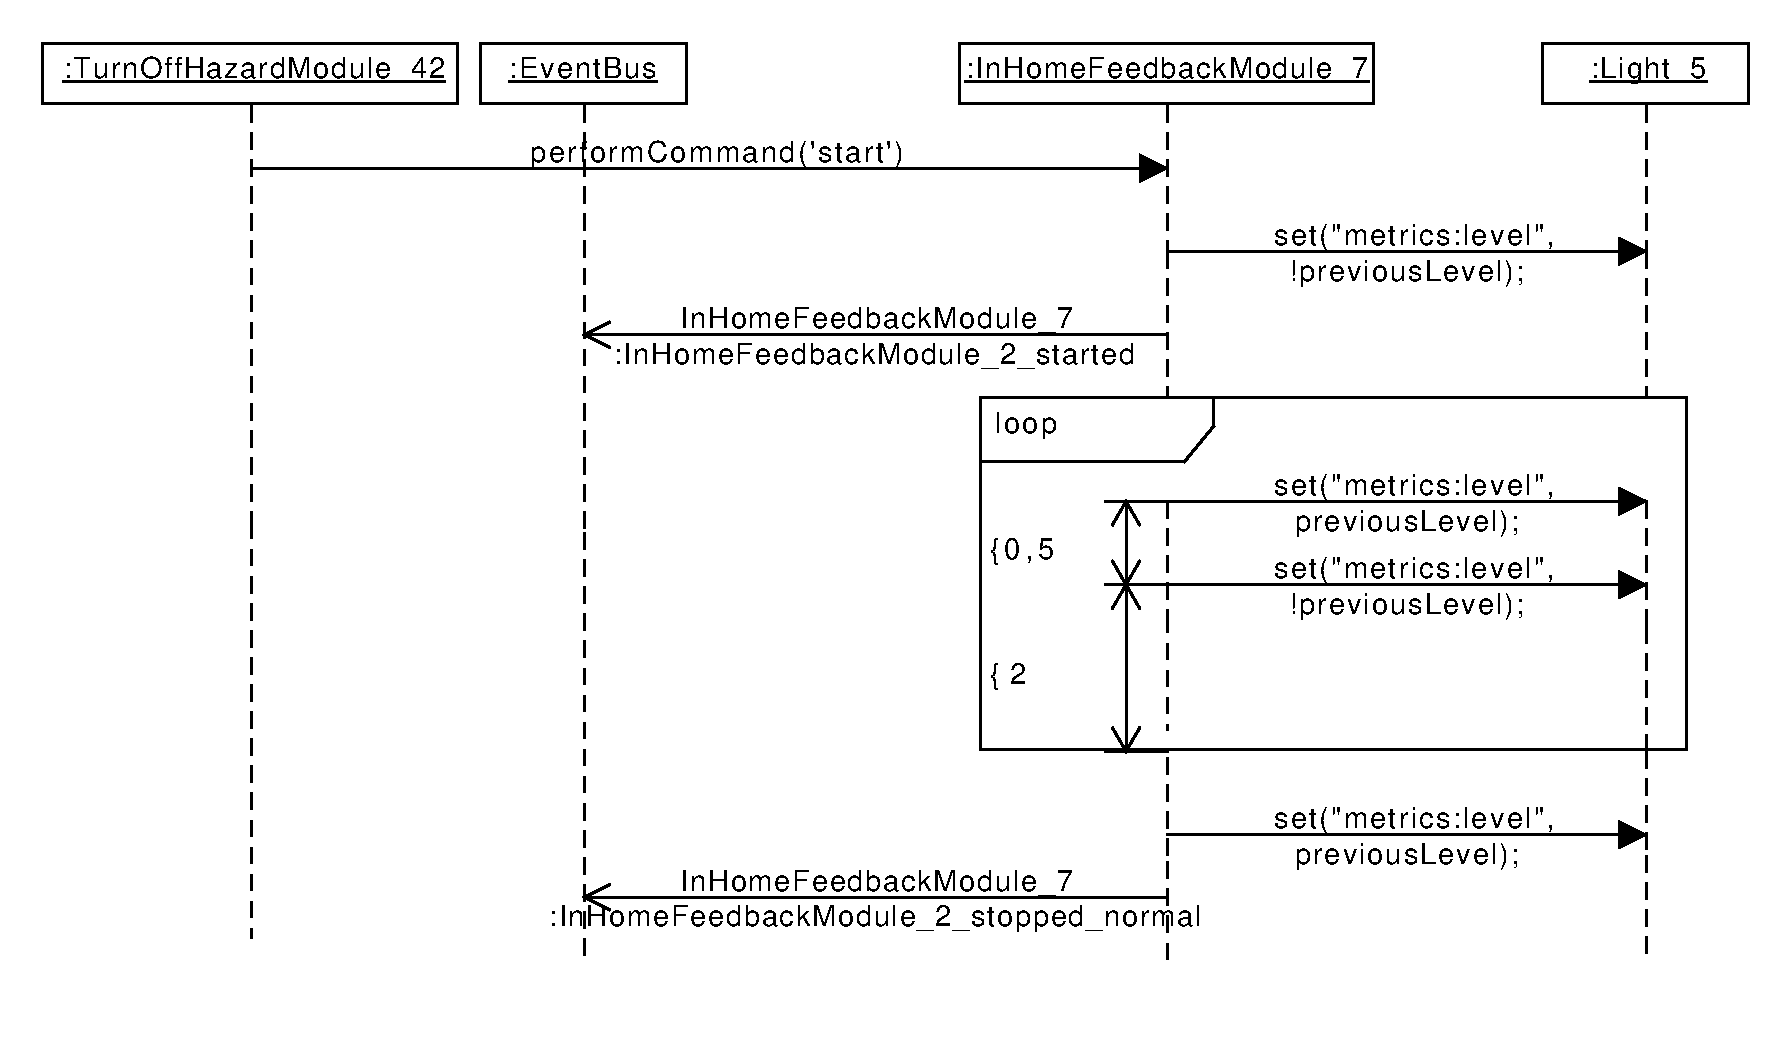
\includegraphics[width=0.9\textwidth]{img/Modulkonzeption/FeedbackSequence.pdf}
	\caption{Sequenzdiagramm – InHomeFeedback-Modul – Beispiel 1}
	\label{fig:feedbackSequence}
\end{figure}

\begin{figure}[h!]
	\centering
	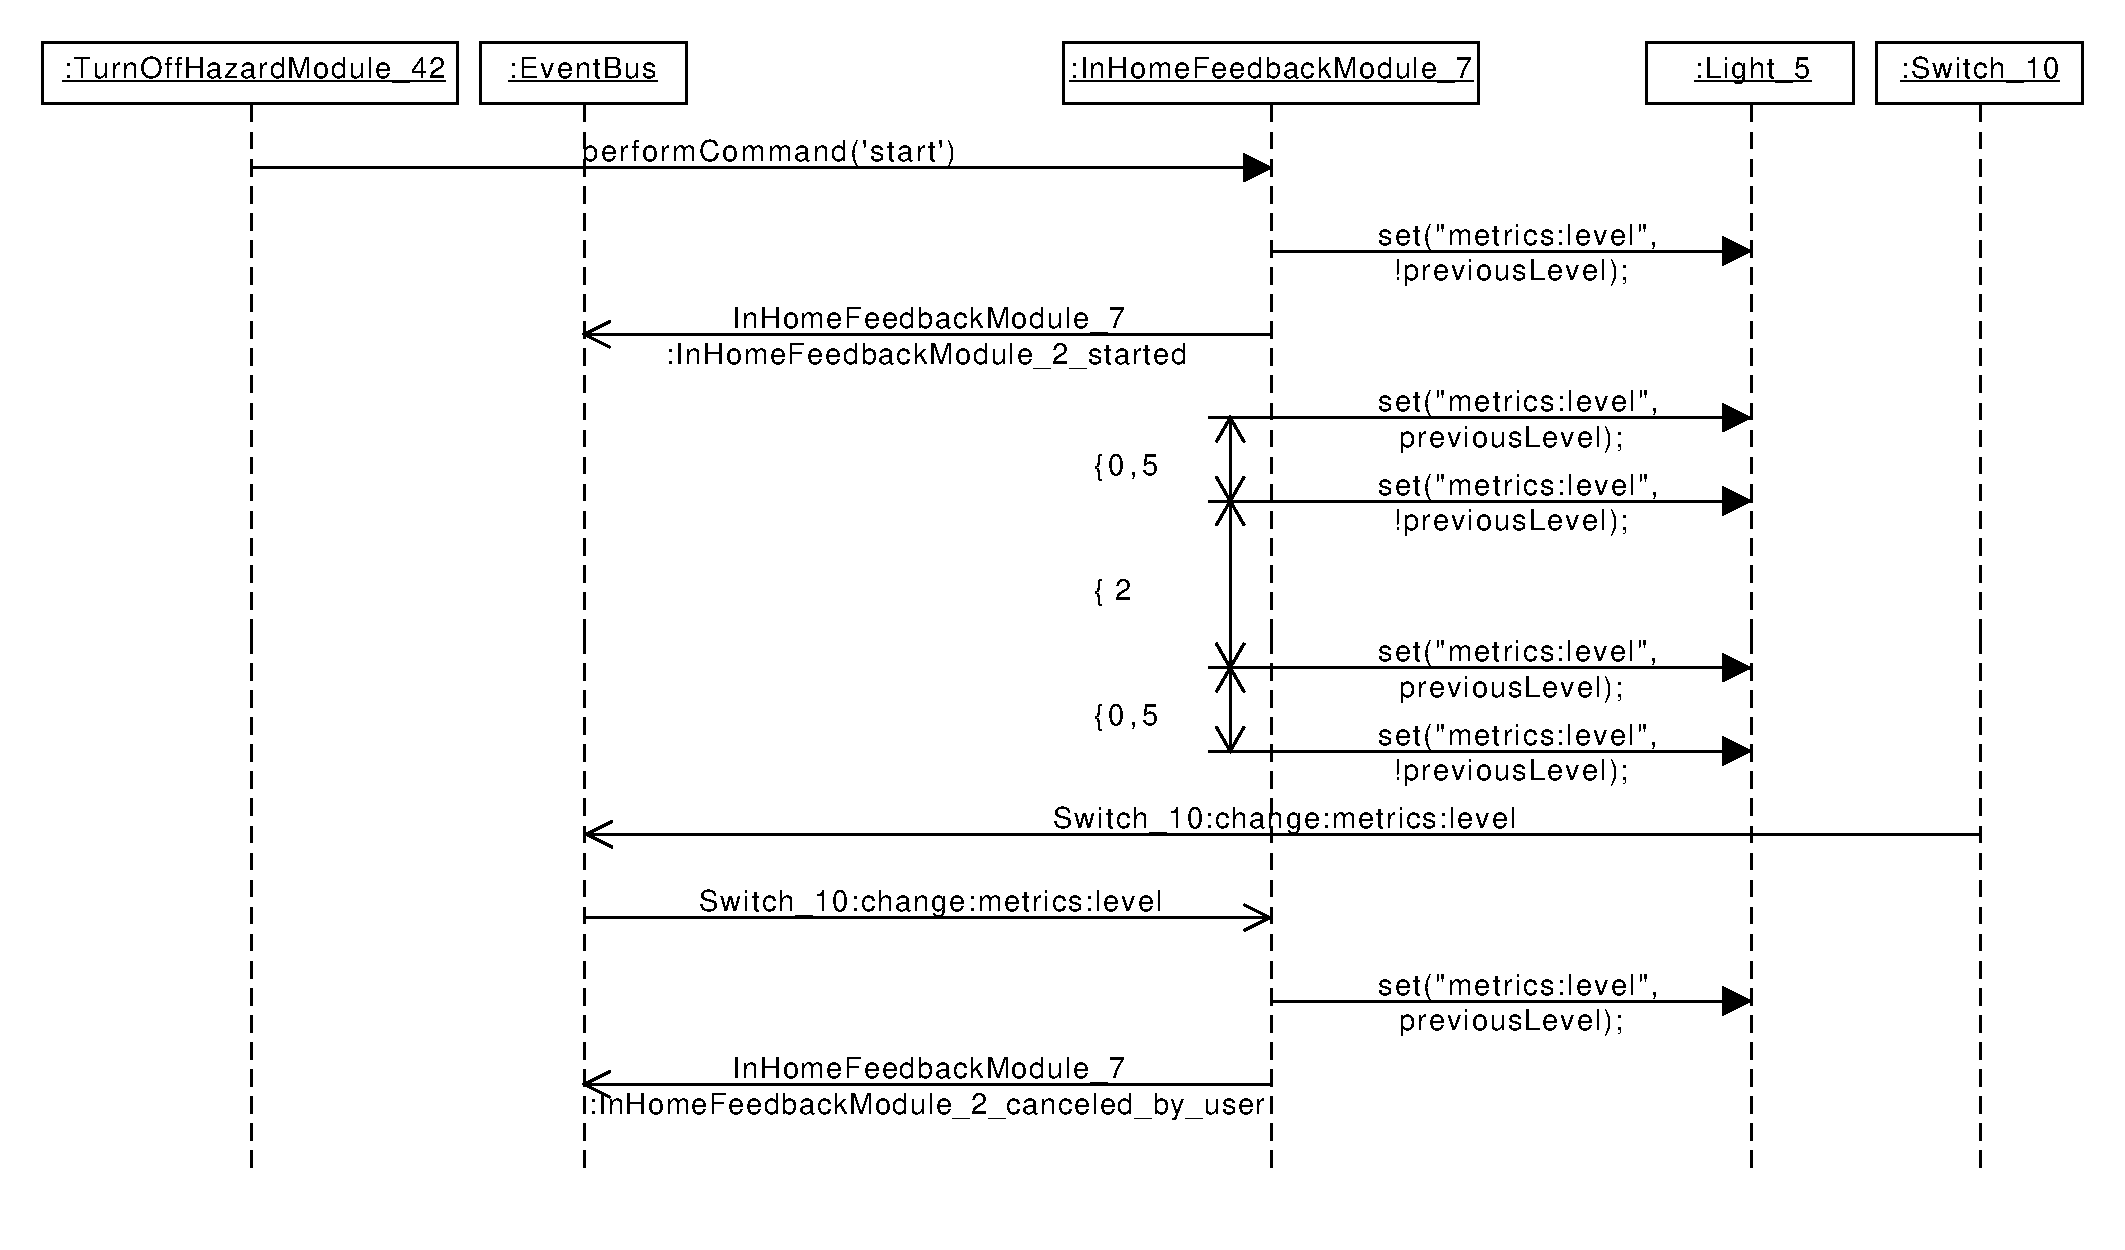
\includegraphics[width=0.9\textwidth]{img/Modulkonzeption/FeedbackSequenceUser.pdf}
	\caption{Sequenzdiagramm – InHomeFeedback-Modul – Beispiel 2}
	\label{fig:feedbackSequenceUser}
\end{figure}


\subsubsection{Konfiguration}

\begin{itemize}
	\item visuelles Feedback
	\begin{itemize}
		\item Typ: Liste [Binary Switch, Multilevel Switch]
		\item Aktion: an/aus/an/aus/an/... bzw. 0-99-0-99-0-...
		\item Erforderlich: nein
		\item Option:
		\begin{itemize}
			\item Frequenz
			\begin{itemize}
				\item Typ: Text
				\item Erforderlich: nein
				\item Standard: 5 Sekunden
			\end{itemize}
		\item spezieller Wert, bspw. RGB (RGB + Warmweiß + Kaltweiß)
		\end{itemize}
	\end{itemize}
	\item akustisches Feedback
	\begin{itemize}
		\item Typ: Liste [*] \textrightarrow{ }bspw. Aeon Labs Sirene \textrightarrow{ }Binary Switch
		\item Aktion: an/aus
		\item Erforderlich: nein
	\end{itemize}
	\item Nachricht
	\begin{itemize}
		\item Vorbedingung: Auswahl von E-Mail bzw. Push-Nachricht
		\item Typ: Liste [Text] (E-Mail-Adresse bzw. URL)
		\item Aktion: HTTP-Request
		\item Erforderlich: nein
	\end{itemize}
	\item Aufruf spezieller Module
	\begin{itemize}
		\item Typ: Liste [Binary Switch, Multilevel Switch] \textrightarrow{ }Device Type der speziellen Module! (deviceType \textrightarrow{ }namespace\_deviceType)
		\item Aktion: an/aus bzw. 0/99
		\item Erforderlich: nein
		\item Option:
		\begin{itemize}
			\item spezieller Wert, bspw. RGB (R + G + B + Warmweiß + Kaltweiß)
		\end{itemize}
	\end{itemize}
	\item HTTP
	\begin{itemize}
		\item Typ: Text
		\item Erforderlich: nein
	\end{itemize}
	\item JavaScript
	\begin{itemize}
		\item Typ: Text
		\item Erforderlich: nein
	\end{itemize}
	\item Raum
	\begin{itemize}
		\item Typ: Text
		\item Erforderlich: ja
	\end{itemize}
	\item Dauer (bis automisch deaktiviert)
	\begin{itemize}
		\item Typ: Text
		\item Erforderlich: nein
		\item Standard: 30 Sekunden
	\end{itemize}
	\item Verzögerungszeit
	\begin{itemize}
		\item Typ: Text
		\item Erforderlich: nein
		\item Standard: 600 Sekunden
	\end{itemize}
	\item Schalter (zum Abbrechen der eingehenden Aktion)
	\begin{itemize}
		\item Typ: Binary Switch
		\item Erforderlich nein
	\end{itemize}

\end{itemize}

\subsubsection{Schnittstellen}
%todo tabelle einfügen

\begin{table}[H]
	\begin{tabularx}{\textwidth}{
			>{\hsize=1.25\hsize}X % 40% of 3\hsize 
			>{\hsize=0.5\hsize\centering}X % 30% of 3\hsize
			>{\hsize=1.25\hsize}X % 40% of 3\hsize
			% sum=3.0\hsize for 3 columns
		}
		\hline
		\textbf{URL}						& \textbf{Parameter}	& \textbf{Beschreibung} \\
		\hline 
		/command/start				
				& duration (opt.) \newline endless=true (opt.) 	
						& Starten des Feedback-Modus (die Durchführung der Aktion wird nicht beeinflusst). Der Parameter "`endless=true"' startet den Feedback-Modus, ohne automatische Terminierung nach einer bestimmten Zeitspanne. \\ 
		\hline 
		/command/stop		
				& - 			 		
						& Stoppen des Feedbackmodus (die Durchführung der Aktion wird nicht beeinflusst). \\
		\hline 
		/command/state
				& - 				
						& Liefert den aktuellen Zustand des Moduls. \\
		\hline
		/command/cancel
				& -
						& Die Aktion abbrechen. \\
		\hline
		/command/defer
				& duration (opt.)
						& Die Aktion um eine bestimmte Zeit verschieben. \\
		\hline
	\end{tabularx}
	\caption{InHomeFeedback-Modul: Schnittstelle ZAutomation}
\end{table}

\begin{table}[H]
	\begin{tabularx}{\textwidth}{
			>{\hsize=1.2\hsize}X 
			>{\hsize=0.8\hsize}X
			% sum=2.0\hsize for 2 columns
		}
		\hline
		\textbf{Event Name}						& \textbf{Beschreibung} \\
		\hline
		[deviceId]:InHomeFeedbackModule\_[roomId]\_started	
				& Feedback-Modus wurde gestartet \\
		\hline 
		[deviceId]:InHomeFeedbackModule\_[roomId]\_stopped\_normal
				& Feedback-Modus wurde nach der vorgegebenen Zeit beendet \\
		\hline
		[deviceId]:InHomeFeedbackModule\_[roomId]\_stopped\_manual
				& Feedback-Modus wurde  gestoppt \\
		\hline
		[deviceId]:InHomeFeedbackModule\_[roomId]\_canceled\_by\_user
				& Feedback-Modus wurde vom Nutzer abgebrochen (aufrufende Komponente sollte dieses Event abfangen und entsprechend reagieren) \\
		\hline
		[deviceId]:InHomeFeedbackModule\_[roomId]\_deferred
				& Aktion wurde um eine bestimmte Zeit aufgeschoben \\
		\hline
		[deviceId]:InHomeFeedbackModule\_[roomId]\_continued
				& - \\
		\hline
	\end{tabularx}
	\caption{InHomeFeedback-Modul: Schnittstellen Event Bus}
\end{table}

\subsubsection{Abhängigkeiten}
\begin{itemize}
	\item Module, für Geräte von Drittanbietern (Philips Hue, Bose, ...)
\end{itemize}

\subsubsection{Interne Speicher}
\begin{itemize}
	\item Raum ID
	\item Zustand - aktiviert, deaktiviert, aufgeschoben
	\item Dauer - falls Modulkonfiguration für den Command überschrieben
	\item Verzögerungszeit - falls Modulkonfiguration für den Command überschrieben
	
\end{itemize}

\subsection{PersonIdentificationModule}
\emph{(von Martin Petzold)}

\subsubsection{Allgemein}
Das PersonIdentificationModule übernimmt die Aufgabe, anhand der Personenanzahl und von Größen- und CO$_2$-Messungen Aussagen darüber zu treffen ob sich erwachsene Personen oder nur Kinder im  jeweiligen Raum befinden. 

\subsubsection{Funktionsweise}
Das Modul benötigt ein PersonCounterModule für den Raum in welchem es angewandt wird. Da der Abgleich der CO$_2$-Messungen nur in Verbindung des Wissens der Personenanzahl ausgewertet werden kann. Weiterhin erfolgt die Größenmessung in Zusammenhang mit der Änderung der im Raum befindlichen Personenanzahl. Somit ergibt sich die Funktionsweise, dass bei Änderung der Personenanzahl im Raum geprüft wird, ob durch die sich an den Raumzugängen durchgeführten Größenmessungen Erwachsene registriert wurden. Danach beginnt als Abgleich der Größenmessung die Messung der CO$_2$ Änderung im Raum. Haben nach den Messvorgängen beide Messgrößen die Anwesenheit eines Erwachsenen registriert gibt das Modul eine Erkennung eines Erwachsenen bekannt. Stellt  allerdings eines der beiden Systeme fest, dass sich kein Erwachsener im Raum befindet oder alle Erwachsenen den Raum verlassen haben, wird das Signal "`kein Erwachsener erkannt"' gesendet. Dieser Ablauf ist auch im Modell (\prettyref{fig:personIdentification}) dargestellt.

\begin{figure}[h!]
	\centering
	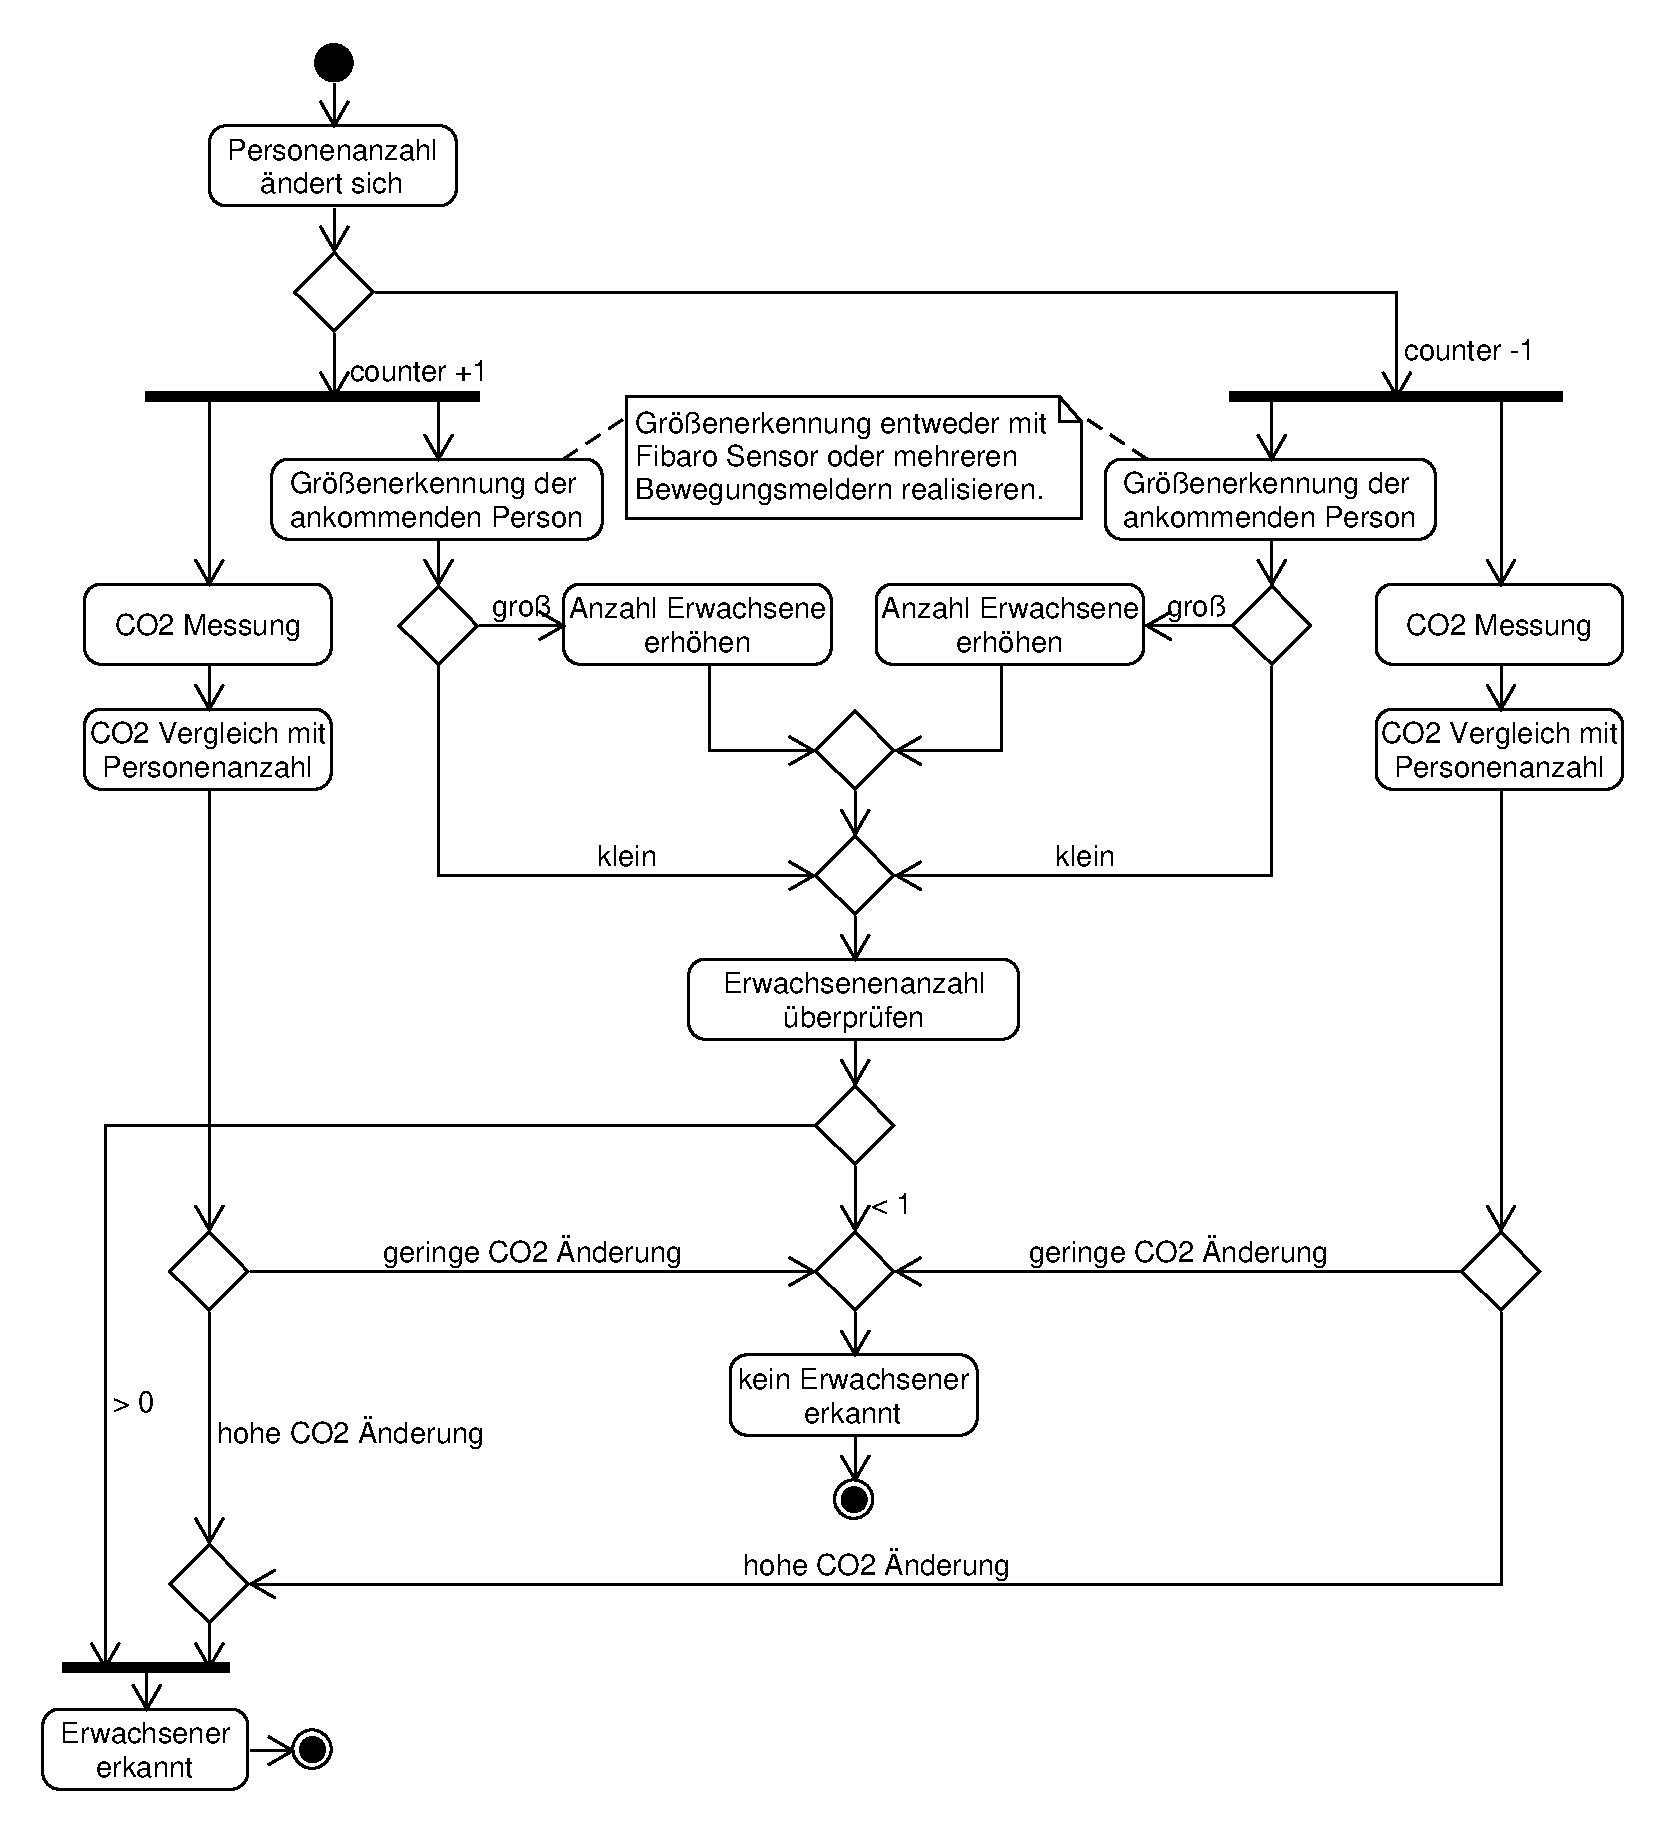
\includegraphics[width=0.9\textwidth]{img/Modulkonzeption/PersonIdentificationStateMachine.pdf}
	\caption{PersonIdentificationModule - Zustandsdiagramm}
	\label{fig:personIdentification}
\end{figure}

\subsubsection{Konfiguration}
\begin{itemize}
	\item CO$_2$-Sensor
	\begin{itemize}
		\item Typ: Multilevel Sensor
		\item erforderlich: ja
		\item Ausgabewert: CO$_2$-Gehalt in ppm
	\end{itemize}
	\item doorWindowContacts
	\begin{itemize}
		\item Typ: Liste[Binary Switches]
		\item erforderlich: ja
		\item Ausgabewert: true/false
	\end{itemize}
	\item peopleSizeMeasurement 
	\begin{itemize}
		\item Typ: Liste[Binary Switches]
		\item erforderlich: ja
		\item Ausgabewert: true/false
	\end{itemize}
	\item roomHeight
	\begin{itemize}
		\item Typ: integer
		\item erforderlich: ja
	\end{itemize}
	\item roomWidth
	\begin{itemize}
		\item Typ: integer
		\item erforderlich: ja
	\end{itemize}
	\item roomLength
	\begin{itemize}
		\item Typ: integer
		\item erforderlich: ja
	\end{itemize}
	\item roomId
	\begin{itemize}
		\item Typ: integer
		\item erforderlich: ja
	\end{itemize}
	\item correctionFactor
	\begin{itemize}
		\item Typ: integer
		\item erforderlich: ja
	\end{itemize}
	\item personCounter
	\begin{itemize}
		\item Typ: Metrik
		\item erforderlich: ja
	\end{itemize}
\end{itemize}

\subsubsection{Schnittstellen}
\begin{table}[H]
	\begin{tabularx}{\textwidth}{
			>{\hsize=1.25\hsize}X % 40% of 3\hsize 
			>{\hsize=0.5\hsize\centering}X % 30% of 3\hsize
			>{\hsize=1.25\hsize}X % 40% of 3\hsize
			% sum=3.0\hsize for 3 columns
		}
		\hline
		\textbf{URL}						& \textbf{Parameter}	& \textbf{Beschreibung} \\
		\hline 
		/command/areThereAdults				
		& - 	
		& Gibt ein Boolean zurück ob sich im Raum Erwachsene befinden. \\ 
		\hline 
		/command/setPersons		
		& Anzahl, Erwachsenenanzahl		% TODO: wie heißen die Parameter wirklich?	 		
		& Setzt die Anzahl der Personen im Raum und startet C02-Messung. \\
		\hline 
		/command/giveData
		& - 				
		& Gibt die Personen-, Erwachsenen- und Kinderanzahl an, die das System registriert hat. \\
		\hline
		/command/setCorrectionFactor
		& Factor
		& Korrekturfaktor für die CO2-Messung. \\
		\hline
		/command/setMeasureTimeDelta
		& TimeDelta
		& Zeitabstand zwischen Änderung des PersonCounter und Höhenmessung, welche noch einen Zusammenhang darstellen. \\
		\hline
		/command/start
		& -
		& \\
		\hline
		/command/stop
		& - 
		& \\
		\hline
		/command/debugOn
		& - 
		& \\
		\hline
		/command/debugOff
		& - 
		& \\
		\hline
	\end{tabularx}
	\caption{PersonIdentification: Schnittstelle ZAutomation}
\end{table}

\begin{table}[H]
	\begin{tabularx}{\textwidth}{
			>{\hsize=1.2\hsize}X 
			>{\hsize=0.8\hsize}X
			% sum=2.0\hsize for 2 columns
		}
		\hline
		\textbf{Event Name}						& \textbf{Beschreibung} \\ %TODO Beschreibung einfügen?
		\hline
		[deviceId]:PersonIdentificationModule\_[roomId]\_started	
		& - \\
		\hline 
		[deviceId]:PersonIdentificationModule\_[roomId]\_stoped
		& - \\
		\hline
		[deviceId]:PersonIdentificationModule\_[roomId]\_adult\_there
		& - \\
		\hline
		[deviceId]:PersonIdentificationModule\_[roomIId]\_no\_adult\_there
		& - \\
		\hline
	\end{tabularx}
	\caption{PersonIdentification: Schnittstellen Event Bus}
\end{table}

\subsubsection{Abhängigkeiten}
\begin{itemize}
	\item PersonCounterModule
\end{itemize}

\subsubsection{Interne Speicher}

\begin{table}[H]
	\begin{tabularx}{\textwidth}{
			>{\hsize=0.85\hsize}X 
			>{\hsize=0.85\hsize}X
			>{\hsize=1.45\hsize}X
			>{\hsize=0.85\hsize}X
			% sum=2.0\hsize for 2 columns
		}
		\hline
		\textbf{Speicher Name}	& \textbf{Datentyp}		& \textbf{Beschreibung}		& \textbf{Initialwert} \\
		\hline
		level					& integer				& Entsprechung des Status "`off"' ist false und "`on"' ist true.	& off \\
		\hline
		status					& boolean				& Status true wenn Erwachsener erkannt, false wenn nicht oder Zustand undefiniert.	& false \\
		\hline
		personCount				& integer				& Interner Zwischenspeicher der Personenanzahl vom zugehörigen Personcounter.	& 0 \\
		\hline
		adultCount				& integer				& Erkannte Erwachsene, welche durch die Größenmessung erkannt wurden.	& 0 \\
		\hline
		room					& integer				& RoomId																& -1 \\
		\hline
		correctionFactor		& integer				& Konstante zur Korrektur,  welche  mit  Messungen multipliziert wird.	& 1 \\
		\hline
		runningState			& boolean				& Zustand ob die Messungen ausgewertet werden oder nicht.			& true \\ 
		\hline
	\end{tabularx}
	\caption{PersonIdentification: Interne Speicher}
\end{table}

%%%%%%%%%%%%%%%%%%%%%%%%%%%%%%%%%%%%%%%%%%%%%%%%%%%%%%%%%%%%%%%%%%%%%%%%%%%%%%%%%%%%%%%%%%%%%%%%%%%%%%%%%%%%%%%%%%%%
\section{Sensorevaluation}
\begin{itemize}
	\item Ergebnisse der Sensorevaluation (je Sensor)
	\item Was funktioniert wie erwartet/was nicht?
	\item Welche technischen Probleme, lassen sich diese einschränken?
	\item Sind Probleme auf Hardware/Software zurückzuführen?
\end{itemize}

\subsection{Fibaro Multisensor}
\emph{(von Philip Laube)}

\subsubsection{Allgemein}
\begin{description}
	\item[Energieversorgung] CR123A battery, 3.6 VDC
	\item[Empfohlene Installationshöhe] 2,4m
	\item[Temperaturreichweite] -20°C bis 100°C
	\item[Temperaturgenauigkeit] 0,5°C bei 0°C bis 40°C
	\item[Lichtintensitätsreichweite] 0-32000 LUX
	\item[Reichweite des Z-Wave Funk] bis zu 50m außerhalb von Gebäuden, bis zu 30m innerhalb von Gebäuden
	\item[Reichweite des Bewegungssensors] 7 Meter
\end{description}

\begin{figure}[h!]
	\centering
	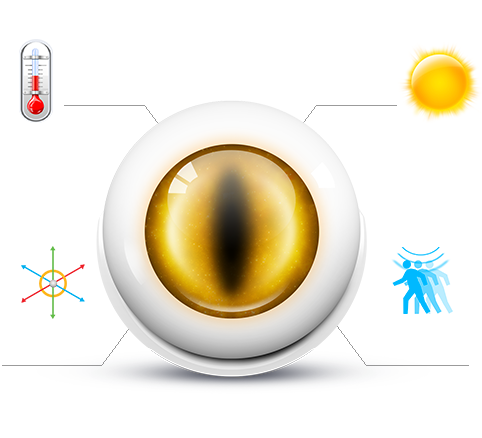
\includegraphics[scale=0.4]{img/Sensorevaluation/FibaroMulti.png}
	\caption{Fibaro Multisensor}
	\label{fig:sensorenFibaroMulti}
\end{figure}

Dieses Gerät ist vielseitig einsetzbar da eine Vielzahl von Sensoren zur Verfügung stehen. Die Bewegungssensoren sollen dazu verwendet werden eine Person beim Durchgehen eines Türdurchganges zu beobachten.
Neben dem Bewegungssensor beinhaltet der Fibaro Multisensor ein Thermometer ein Lichtsensor sowie einen Erschütterungssensor.
Der Erschütterungssensor wird standardmäßig als Diebstahlschutz verwendet um zusätzliche Ereignisse auszulösen.

\begin{figure}[h!]
	\centering
	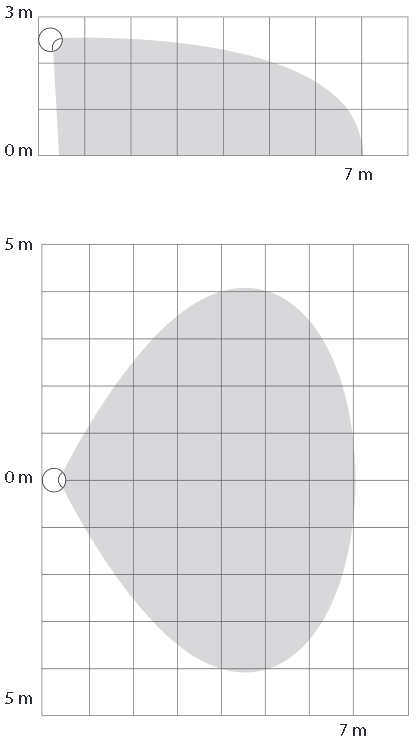
\includegraphics[scale=0.4]{img/Sensorevaluation/FibaroMultiRange.png}
	\caption{Reichweite des Bewegungssensors}
	\label{fig:sensorenFibaroMultiRange}
\end{figure}
 
\begin{figure}[h!]
	\centering
	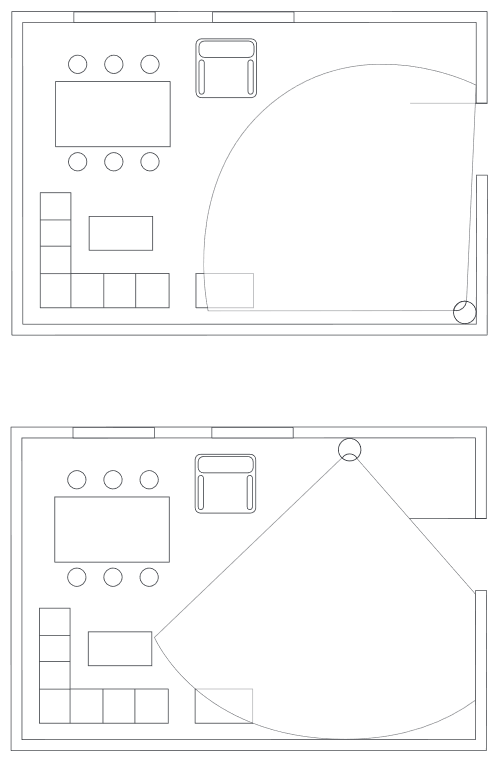
\includegraphics[scale=0.4]{img/Sensorevaluation/FibaroMultiExamples.png}
	\caption{Generelle Installationspunkte zum Beobachtung eines Raumes}
	\label{fig:sensorenFibaroMultiExamples}
\end{figure}

\subsubsection{Praxistest – Türdurchgang}
Für die Konfiguration der Geräte müssen folgende Anpassungen vorgenommen werden.

Parameter 1 = 8, Parameter 2 = 0, Parameter 6 = 1s

Das hat dann zur Folge das jede Sekunde ein Event geworfen wird. Mit diesen Parametern wird zudem jede kleinste Bewegung eines Menschen, die für eine solche Funktion notwendig ist, erkannt. Nun werden pro Raum ein Sensor vor die Tür mit Sicht zur Tür befestigt. Diese werden dann später von einem Modul der diesen Raumdurchgang implementiert benutzt.

\subsubsection{Parameterübersicht}
\begin{description}
	\item [Parameter 1] Wird benutzt um die Sensitivität des Sensors einzustellen und ist ein Wert zwischen 8 und 255 wobei ein kleinerer Wert eine höhere Sensitivität zur Folge hat.

	\item [Parameter 2] Gibt einen Wert an um den Bewegungssensor eine gewisse Zeit nach einem Erkennen von Bewegung blind zu machen. Dabei ist der Wertebereich hier zwischen 0 und 15 wobei eine Einheit eine halbe Sekunde entspricht. So entspricht ein Wert von 0 0,5 Sekunden während ein Wert von 15 8 Sekunden entspricht.
	\item [Parameter 6] Nach wie vielen Sekunden wird im Hauptcontroller (bei uns Z-Way) der Bewegungssensor nach einem Auslösen des Sensors wieder auf inaktiv gesetzt. Der Countdown wird erneut zurückgesetzt sofern eine neue Bewegung erkannt wird. Um dies entgegenzuwirken soll Parameter 2 weiter angepasst werden.
\end{description}

Mit diesen eingestellten Parametern kann nun bei einem Türdurchgang mit zwei solcher Bewegungssensoren eine Person zuverlässig erkannt werden. Ein Personenzähler hält dabei die erkannten Werte dauerhaft. 

\begin{description}
	\item [Parameter 8] Gibt nur an zu welcher Tageszeit der Sensor aktiv sein soll. Bei dem Wert 0 ist er den ganzen Tag aktiv, bei dem Wert 1 nur am Tag und bei einem Wert von 2 nur bei Nacht. Hinzuzufügen ist hier das die Bestimmung ob Tag oder Nacht ist durch den internen Lichtsensor realisiert wird. Dieser Wert kann unter dem Parameter 9 eingestellt werden.
	\item [Parameter 20] Die Sensitivität des Erschütterungssensor (Wertebereich 0 – 122 = 0.08 – 2g = Wert * 0.016g)
	\item [Parameter 22] Alle wie viele Sekunden wird der Sensor zurückgesetzt und ein neuer Erschütterungswert kann gesendet werden.
	\item [Parameter 26] Der Alarm kann hiermit über einen Broadcast an alle Geräte in der Reichweite gesendet werden, sofern diese einen solchen Broadcast empfangen können.
	\item [Parameter 40] Die minimale Änderung des einfallenden Lichts in Lux um den aktuellen Lux Wert zu senden
	\item [Parameter 42] alle wie viele Sekunden soll der Lux Wert gesendet werden, unabhängig von der Änderung des einfallenden Lichts
	\item [Parameter 60] Die minimale Änderungen der Temperatur bis der aktuelle Wert gesendet wird
	\item [Parameter 62] Alle wie viele Sekunden wird die Temperatur gemessen
	\item [Parameter 64] alle wie viele Sekunden soll der Temperatur Wert gesendet werden, unabhängig von der Änderung der Temperatur
	\item [Parameter 66] Anpassung der erkannten Temperatur zur Kalibrierung des Geräts
	\item [Parameter 80+] Alle Einstellungen für die LED des Auges
\end{description}

\subsubsection{Weitere Funktionalitäten}
Mit dem Parameter 24 = 4 und einer eingestellten minimalen Vibration in Parameter 20 sowie einem Intervall in Parameter 22 in Sekunden ein Seismograph eingestellt werden.

Dabei wird ab dem Erreichen des Minimalwertes intervallmäßig der erkannte Erschütterungswert gesendet solang die Erschütterung über dem Minimalwert anhält.
%TODO Quellen ergänzen
%Weitere Einstellungen, sowie alle konkreten Wertebereiche sind in der Anleitung Motion-Sensor_EN_5.3.14.pdf zu finden.

%http://www.fibarouk.co.uk/counting-people-using-two-motion-sensors/
%http://www.fibaro.com/manuals/en/Motion-Sensor/Motion-Sensor_EN_5.3.14.pdf
%http://www.fibaro.com/de/the-fibaro-system/motion-sensor
%http://www.fibaro.com/sites/all/themes/fibaro/images/motion-sensor/en/motion_sensor_02.png


\subsection{Fibaro Wall Plug (FGWPx-102) – Zwischenstecker}

\emph{(von Patrick Hecker)}
\subsubsection{Funktionalität}
\begin{itemize}
	\item ZWave kompatibler Zwischenstecker in Form eines Steckdosenadapters
	\item Steuerung elektrischer Geräte (max. 2,5 kW)
	\item Messung von Wirkleistung und Stromverbrauch
	\item Anzeige über Schaltzustand und Stromverbrauch über Mehrfarben-LED-Ring
	\item Steuerung am Gerät über Taste
\end{itemize}
\subsubsection{Z-Way Elemente}
\begin{itemize}
	\item Fibaro Wall Plug
	\begin{itemize}
		\item Binary Switch
		\item Steuerung des Schaltzustandes
	\end{itemize}
	\item Meter Electric
	\begin{itemize}
		\item Sensor Multilevel
		\item Stromverbrauch in kW
	\end{itemize}
	\item Sensor Power
	\begin{itemize}
		\item Sensor Multilevel
		\item Wirkleistung in W
	\end{itemize}
\end{itemize}

\subsubsection{Konfiguration}

\paragraph{Immer An - Funktion}
\begin{itemize}
	\item Parameter 1:
	\begin{description}
		\item [0] aktiviert,
		\item [1] deaktiviert
	\end{description}
\end{itemize}

\paragraph{Der Zwischenstecker kann auf Z-Wave Netzwerk Alarm reagieren}
\begin{description}
	\item [Parameter 34:] Welcher Alarm soll Reaktion auslösen?
	\begin{description}
		\item [1] genereller Alarm
		\item [2] Rauchalarm
		\item [4] CO Alarm
		\item [8] CO$_2$ Alarm
		\item [16] Temperaturalarm
		\item [32] Überflutungsalarm
		\item [63] auf jeden Alarm reagieren
	\end{description}
	\item [Parameter 35:] Reaktion auf Alarm
	\begin{description}
		\item [0] keine Reaktion,
		\item [1] Schaltzustand ein,
		\item [2] Schaltzustand aus, zyklischer Wechsel (an/aus) jede Sekunde	
	\end{description}
	\item [Parameter 39:] Dauer der Reaktion
	\begin{itemize}
		\item 1 – 65536 Sekunden
	\end{itemize}
\end{description}

\paragraph{Aussenden verschiedener Reports}
\begin{description}
	\item [Parameter 40 - 45] nur bei Änderung des Stromverbrauchs
	\item [Parameter 47] periodisch, ohne Berücksichtigung des Stromverbrauchs
	\begin{description}
		\item [Parameter 40:] Sofortiger Report über Stromverbrauch (W)
		\begin{itemize}
			\item 1 – 100 \%
		\end{itemize}
		\item [Parameter 42:] Standardmäßiges Aussenden von Reports über den Stromverbrauch
		\begin{itemize}
			\item 1 – 100 \%
		\end{itemize}
		\item [Parameter 43:] Zeitintervall zum Senden eines Reports über den Stromverbrauch
		\begin{itemize}
			\item 1 – 254 Sekunden (bezieht sich auf Parameter 42)
		\end{itemize}
		\item [Parameter 45:] Änderung in der Stromaufnahme durch gesteuerte Geräte (kWh)
		\begin{itemize}
			\item 1 – 254 (0,01 – 2,54 kWh)
		\end{itemize}
		\item [Parameter 47:] Zeitintervall zwischen den Reports über die momentane Wirkleistung und den Stromverbrauch
		\begin{itemize}
			\item 1 – 65534 Sekunden
			\item Erklärung: Report im Zeitintervall, ohne Änderung im Verbrauch!
		\end{itemize}
		\item [Parameter 49:] Messen des Eigenstromverbrauchs des Wall Plug Moduls
		\begin{description}
			\item [0] keine Einbeziehung des Eigenstromverbrauchs
			\item [1] inklusive Eigenstromverbrauch
		\end{description}
	\end{description}
\end{description}

\paragraph{Einstellungen zu Assoziationsgruppe 2}
\begin{description}
	\item [Parameter 50:] Unterer Leistungsschwellwert
	\item [Parameter 51:] Oberer Leistungsschwellwert
	\item [Parameter 52:] Konfiguration des Verhaltens beim Überschreiten der festgelegten Leistungsschwellwerte
\end{description}

\paragraph{Farbeinstellungen}
\begin{description}
	\item[Parameter 60:] Leistungsschwellwert für violettes Blinken
	\begin{itemize}
		\item 1000 – 32000 (100 – 3200 W)
	\end{itemize}
	\item [Parameter 61:] LED-Ring-Farbe im Einschaltzustand
	\item [Parameter 62:] LED-Ring-Farbe im Ausschaltzustand
	\item [Parameter 63:] LED-Ring-Farbe bei Z-Wave-Alarmmeldung
	\item [Parameter 61 - 63:] Farbwerte
	\begin{description}
		\item [1] White
		\item [2] Red
		\item [3] Green
		\item [4] Blue
		\item [5] Yellow
		\item [6] Cyan
		\item [7] Magenta
		\item [8] Farbe aus
	\end{description}
\end{description}
Weitere Informationen (auch technische Details) sind dem Handbuch zu entnehmen.


\subsection{Aoetec Multisensor Sensor}
\emph{(von Alexander Keller)}

\subsubsection{Allgemein}

Im Bereich Smarthome hat man eine riesige Auswahl von verschiedenen Sensoren. Je nach Bedarf bieten die Multisensoren verschiedene Funktionalitäten welche Bewegungen, Raumtemperatur, Licht oder andere registrieren können. Der Aeotec Sensor erfasst 6 verschiedene Messwerte. Die Sensoren messen Raumtemperatur, Lichtstärke, Luftfeuchtigkeit, Bewegung, UV-Sensor und Vibration. Diese Werte überträgt der Multisensor mit einer drahtlosen Kommunikationsschnittstelle names Z-Wave.

In unserem Projekt kommt dieser Sensor zum Einsatz, um das Alarm Modul, Personenidentifikationsmodul und Gefahrenmodul mithilfe seiner Sensortechnik zu unterstützen.


\subsubsection{Konfigurationsmöglichkeiten}

Nachdem man das Gerät erfolgreich im Z-Way Home Center hinzugefügt hat, besteht die Möglichkeit den Multisensor über die Expert-UI zu konfigurieren.

\begin{figure}[h!]
	\centering
	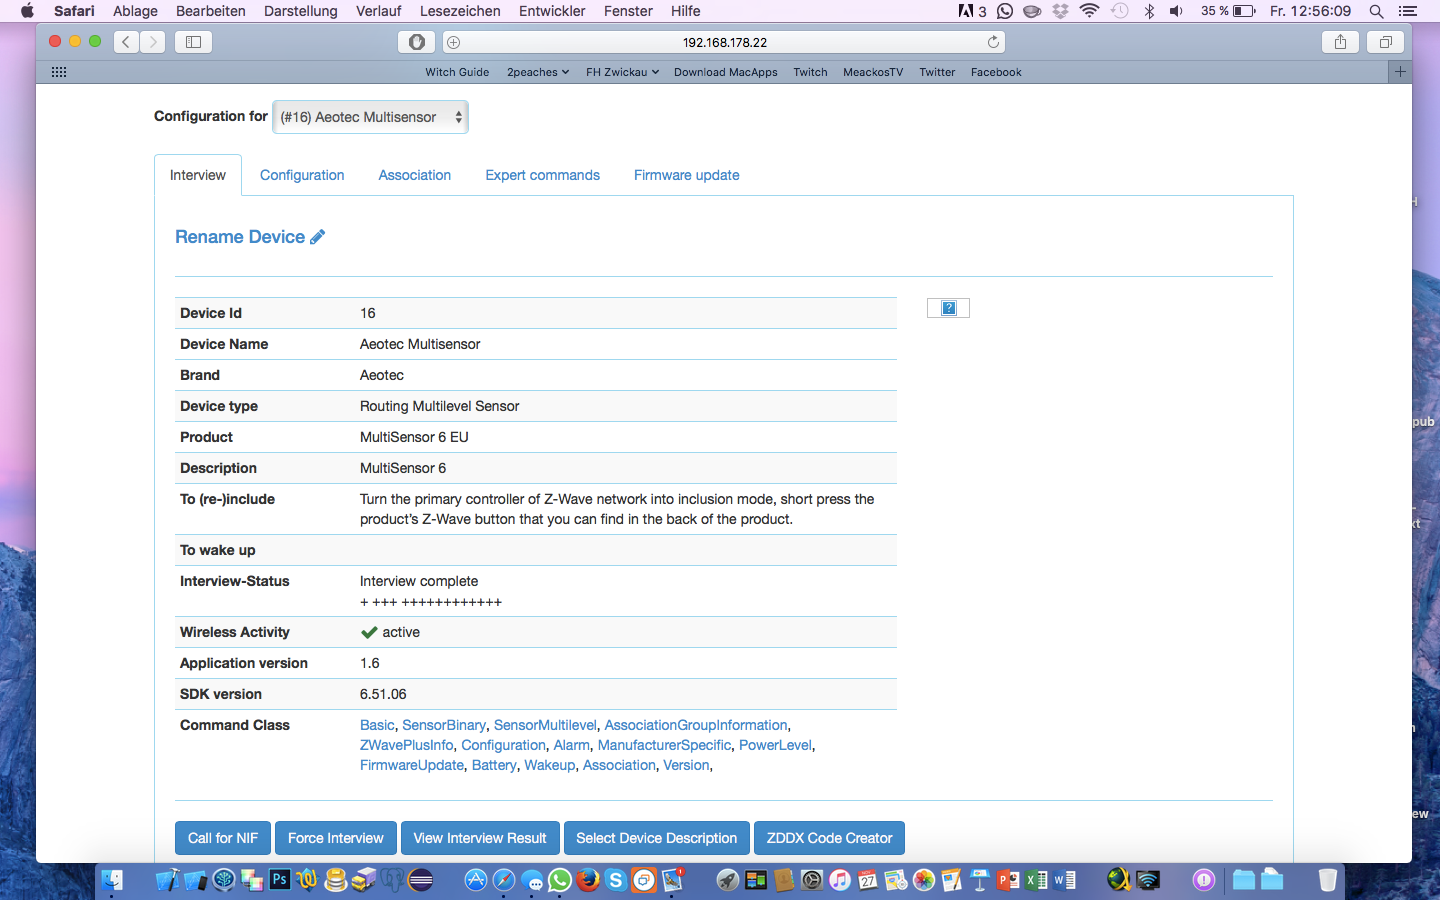
\includegraphics[width=0.9\textwidth]{img/Sensorevaluation/AeoScreenshot.png}
	\caption{Übersichtsseite des Aeotec Multisensor}
	\label{fig:sensorenAeoScreenshot}
\end{figure}

Der Z-Way Server erstellt automatisiert eine Übersichtsseite nachdem der Sensor erfolgreich hinzugefügt wurde. In diesem Reiter besteht die Möglichkeit das Gerät umzubenennen, Netzwerkstatus abzurufen, \gls{sdk} Version.

Im Reiter „Configuration“ findet man alle Einstellungsmöglichkeiten die der Sensor bietet. In der nachfolgenden Tabelle, finden sie alle Konfigurationsoptionen.
\begin{longtabu} to \linewidth {
		>{}X
		>{}X
		>{}X
	}
	
	% ----------- headings -----------
	\hline
	\textbf{Name}							& \textbf{Optionen}		& \textbf{Beschreibung} \\
	\hline
	\endfirsthead
	\hline
	\textbf{Name}							& \textbf{Optionen}		& \textbf{Beschreibung} \\
	\hline
	\endhead
	\hline 
	% ----------- end headings -----------
	% ----------- begin footer -----------
	\multicolumn{3}{r}{{Fortsetzung auf nächster Seite}}  \\ 
	%\hline
	\endfoot
	%\hline
	\endlastfoot
	% ----------- end footer -----------
	Wake Up 10 Minutes when	batteries are inserted	
			& No \newline Yes				
					& Der Sensor "`erwacht"' alle 10 Minuten, wenn Batterien eingelegt sind. \\ 

	\hline 
	On Time									& X Minuten	 		& Wie lang sollen die verschiedenen Sensoren den aktuellen Wert speichern bevor diese aktualisiert werden \\ 
	\hline
	Enable/Disable the function of motion Sensor &
			(0) disable \newline
			(1) enable, the current PIR sensitivity level=1. (minimum level) \newline
			(2) enable, the current PIR sensitivity level = 2. \newline
			(3) enable, the current PIR sensitivity level=3. \newline
			(4) enable, the current PIR sensitivity level=4. \newline
			(5) \uline{enable, the current PIR sensitivity level=5. (maximum level)} \newline &
					Es besteht die Möglichkeit den Bewegungssensor zu deaktivieren \& die Intensität einzustellen \\
	\hline
	Motion Detection &
			(1) \uline{Send Basic Set CC.} \newline
			(2) Send Sensor Binary Report CC. &
					Welchen Standard soll der Aeotec Sensor sende, wenn der Bewegungssensor ausgelöst wurde \\
	\hline
	Low Batterie Value &
			X \% &
					Ab welchen prozentualen Wert soll der Sensor bescheid geben, wenn der Batteriestand niedrig ist. \\
	\hline
	Reports for Parameter 41 – 44 &
			(0) \uline{disable} \newline
			(1) enable &
					Diese Funktionalität dient dazu um bestimmte Schwellenwerte in bestimmten Zeitabständen zu an den Z-Way Server zu senden. (Netzwerktraffic) \\
	\hline
	Humidity Automatic Report &
			X Schwellenwert &
					Festlegen eines Schwellenwertes für den Feuchtigkeitssensor \\
	\hline
	Luminance Automatic Report &
			X Luminanz &
					Festlegen eines Schwellenwertes für den Lichtsensor \\
	\hline
	Battery Automatic Report &
			X Prozent &
					Festlegen eines Schwellenwertes für die Batterieänderung \\
	\hline
	Threshold change in ultraviolet to induce an automatic report. &
			X Schwellenwert &
					Festlegen eines Schwellenwertes für Ultra Violettes Licht \\
	\hline
	Low Temperature Alarm Report &
			(0) Disable to send the alarm report of low temperature \newline
			(1) Enable to send the alarm report of low temperature &
				 Bericht wenn die Temperatur unter 15 Grad fällt. \\
	\hline
	Unsolicitate reports interval for timing groups 1 / 2 / 3 &
			X Sekunden &
					Alle X Sekunden sendet der Motion Sensor einen Bericht. \\
	\hline
	Lock Configuration &
			(0) Disable all configuration parameters to be locked.\newline
			(1) Enable all configuration parameters to be locked. &
					Alle Änderungen von Parametern werden gespeichert. \\
	\hline
	Reset to default factory setting &
			(1) Resets all configuration parameters to default setting. \newline
			(1431655765) Reset the product to default factory setting and be excluded from the Z-wave network. &
					Hier besteht die Möglichkeit den Mutlisensor komplett auf Werkseinstellung zurückzusetzen \& ihn anschließend aus dem Z-Way Netzwerk zu entfernen. \\
	\hline
	WakeUp Settings &
			X Sekunden &
					Nach wie vielen Sekunden der Sensor erwachen sollen, wenn keine Aktivität vorhanden war \\
	\hline
		
\caption{Konfiguration des Aeotec-Sensors} \\
\end{longtabu}

\subsubsection{Praxistest}
Um das Gerät ausführlich testen zu können, ist es notwendig als ersten Schritt die Batterien einzulegen. Der Motion Sensor von Aeotec benötigt 4x AAA Batterien, welche mindestens 12 Monate lange halten.
\subsubsection{Motion Sensor}
Die effektive Reichweite des Bewegungssensors ist begrenzt. Anhang der Skizze ist zu erkenne, dass der Radius bei einer Höhe von 3 Metern, maximal 10 Meter beträgt.

\begin{figure}[h!]
	\centering
	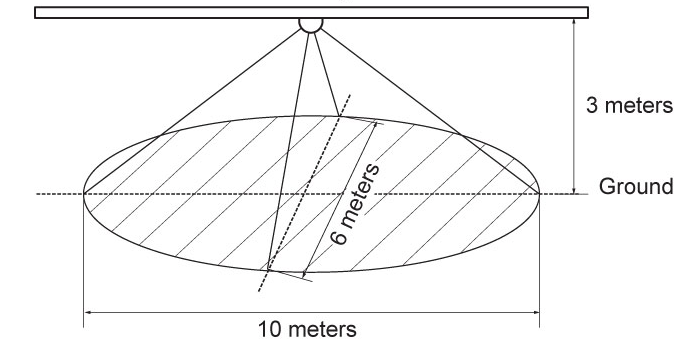
\includegraphics[width=0.9\textwidth]{img/Sensorevaluation/AeoMeter1.png}
	\caption{Bewegungssensor in der Praxis ohne Hindernisse}
	\label{fig:sensorenAeoMeter1}
\end{figure}

Falls eine Wand oder andere Hindernisse im Weg sind muss die Berechnung des Durchmesser, sowie die Reichweite des Bewegungssensors individuell angepasst werden. Im folgenden Beispiel hängt der Sensor von Aeotec nicht an der Decke, sondern ist an einer Wand befestigt.

\begin{figure}[h!]
	\centering
	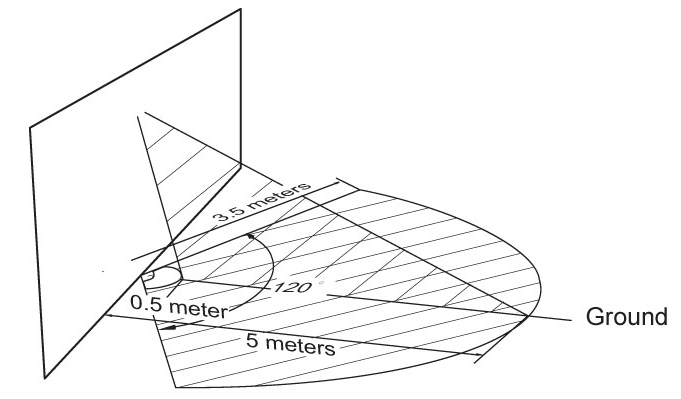
\includegraphics[width=0.9\textwidth]{img/Sensorevaluation/AeoMeter2.png}
	\caption{Bewegungssensor in der Praxis an einer Wand}
	\label{fig:sensorenAeoMeter2}
\end{figure}

\subsubsection{Temperatur}
\begin{figure}[h!]
	\centering
	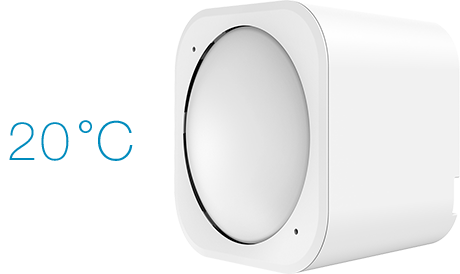
\includegraphics[width=0.5\textwidth]{img/Sensorevaluation/AeoTemp.png}
	\caption{Aoetec Temperatursensor}
	\label{fig:sensorenAeoTemp}
\end{figure}

Der Multisensor der Firma Aeotec bietet die Möglichkeit dem Nutzer die aktuelle Raumtemperatur anzuzeigen. Im Praxistest hat sich gezeigt, dass die Temperatur immer 1 – 3 Grad Celsius zu viel angezeigt hat. Eine Kalibrierung des Sensors ist laut Konfigurationsmöglichkeiten (siehe oben) nicht möglich. Das wiederum heißt, dass der Nutzer seinen Schwellenwert immer um den Mittelwert 2 Grad Celsius anheben sollte.

\subsubsection{Lichtsensor}
\begin{figure}[h!]
	\centering
	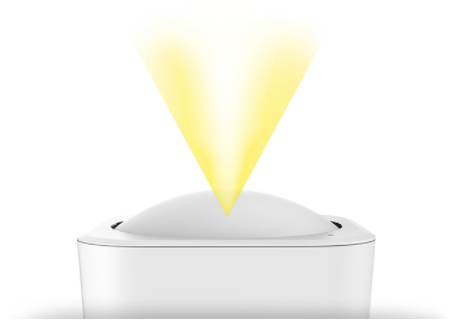
\includegraphics[width=0.5\textwidth]{img/Sensorevaluation/AeoLight.png}
	\caption{Aoetec Lichtsensor}
	\label{fig:sensorenAeoLight}
\end{figure}

In der Praxis erwies sich sich der Lichtsensor für sehr zuverlässig. Der Anwendungsbereich dafür wäre eine automatisierte Rollladensteuerung oder Lampensteuerung.

\subsubsection{Luftfeuchtigkeitssensor}
\begin{figure}[h!]
	\centering
	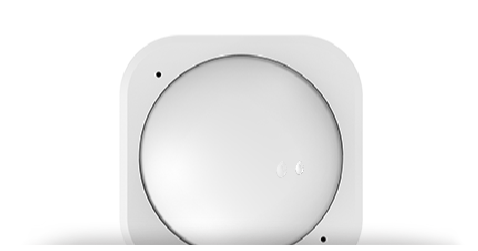
\includegraphics[width=0.5\textwidth]{img/Sensorevaluation/AeoHum.png}
	\caption{Aoetec Feuchtigkeitssensor}
	\label{fig:sensorenAeoHum}
\end{figure}

Der Aoetec Sensor besitzt einen Luftfeuchtigkeitssensor mit diesem man die Luftfeuchtigkeit zwischen 0\% und 100\% messen kann. Die praktische Anwendung wäre eine automatisierte Tür- \& Fenstersteuerung, welches ein perfektes Klima im Raum ermöglicht.

\subsubsection{Vibrationssensor}
\begin{figure}[h!]
	\centering
	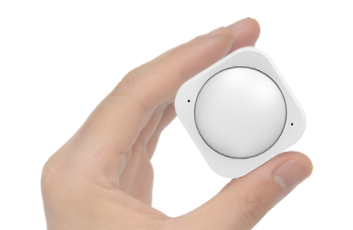
\includegraphics[width=0.5\textwidth]{img/Sensorevaluation/AeoVib.png}
	\caption{Aoetec Vibrationssensor}
	\label{fig:sensorenAeoVib}
\end{figure}

Durch den eingebauten seismischen Sensor überwacht dieser Erschütterungen und Vibrationen. Diese Funktionalität bietet sich bestens um Alarm diesen Vibrationssensor in ein Alarmmodul zu integrieren damit dieser bei ungewöhnlichen Erschütterungen Alarm schlägt.

\subsubsection{UV Sensor}
\begin{figure}[h!]
	\centering
	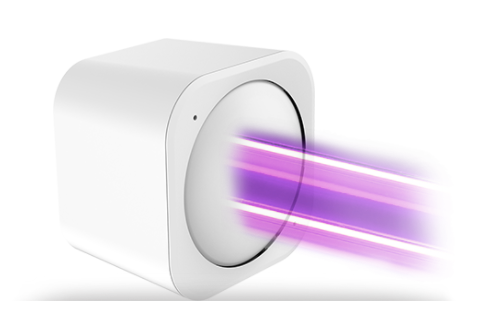
\includegraphics[width=0.5\textwidth]{img/Sensorevaluation/AeoUV.png}
	\caption{Aoetec UV-Sensor}
	\label{fig:sensorenAeoUV}
\end{figure}

Ab einen bestimmten Anteil von ultravioletten Licht ist dieses sehr schädlich für das Auge. Um sich davor zu schützen, sind elektrische Jalousien oder Rollläden notwendig.



\subsection{Philio 4-in-1 Multisensor}
\emph{(von Tobias Weise)}
\subsubsection{Allgemein}
Im Bereich Smart Home hat man eine riesige Auswahl von verschiedenen Sensoren. Je nach Bedarf biete der Philio 4-in-1 Multisensor verschiedene Funktionalitäten, welche Bewegungen, Tür- und Fenster öffnen bzw. schließen, Licht- oder Temperaturänderungen registrieren können. Der Philio 4-in-1 Multisensor ist somit in der Lage 4 verschiedene Messwerte zu erfassen. Diese Werte überträgt der Multisensor mit einer drahtlosen Kommunikationsschnittstelle names Z-Wave an den Z-Way Server.

Im Rahmen des Projektes kommt dieser Sensor zum Einsatz, um das Öffnen und Schließen der Wohnungstüre, sowie Bewegungen innerhalb des Raumes zu registrieren. Dabei findet er hauptsächlich in den Modulen „LockDoorModule“, „PersonCounterModule“ und „StandbyModule“ Verwendung. Durch die vielseitigen Einstellungsmöglichkeiten der Parameter des Sensors, wird nachfolgend eine Evaluierung der Möglichkeiten, die man bei der Parametereinstellung hat, durchgeführt.

\subsubsection{Konfigurationsmöglichkeiten}
Nachdem man den Sensor erfolgreich in das Z-Way Home Center eingefügt hat, besteht die Möglichkeit, den Multisensor über die Expert-UI zu konfigurieren.


\begin{figure}[h!]
	\centering
	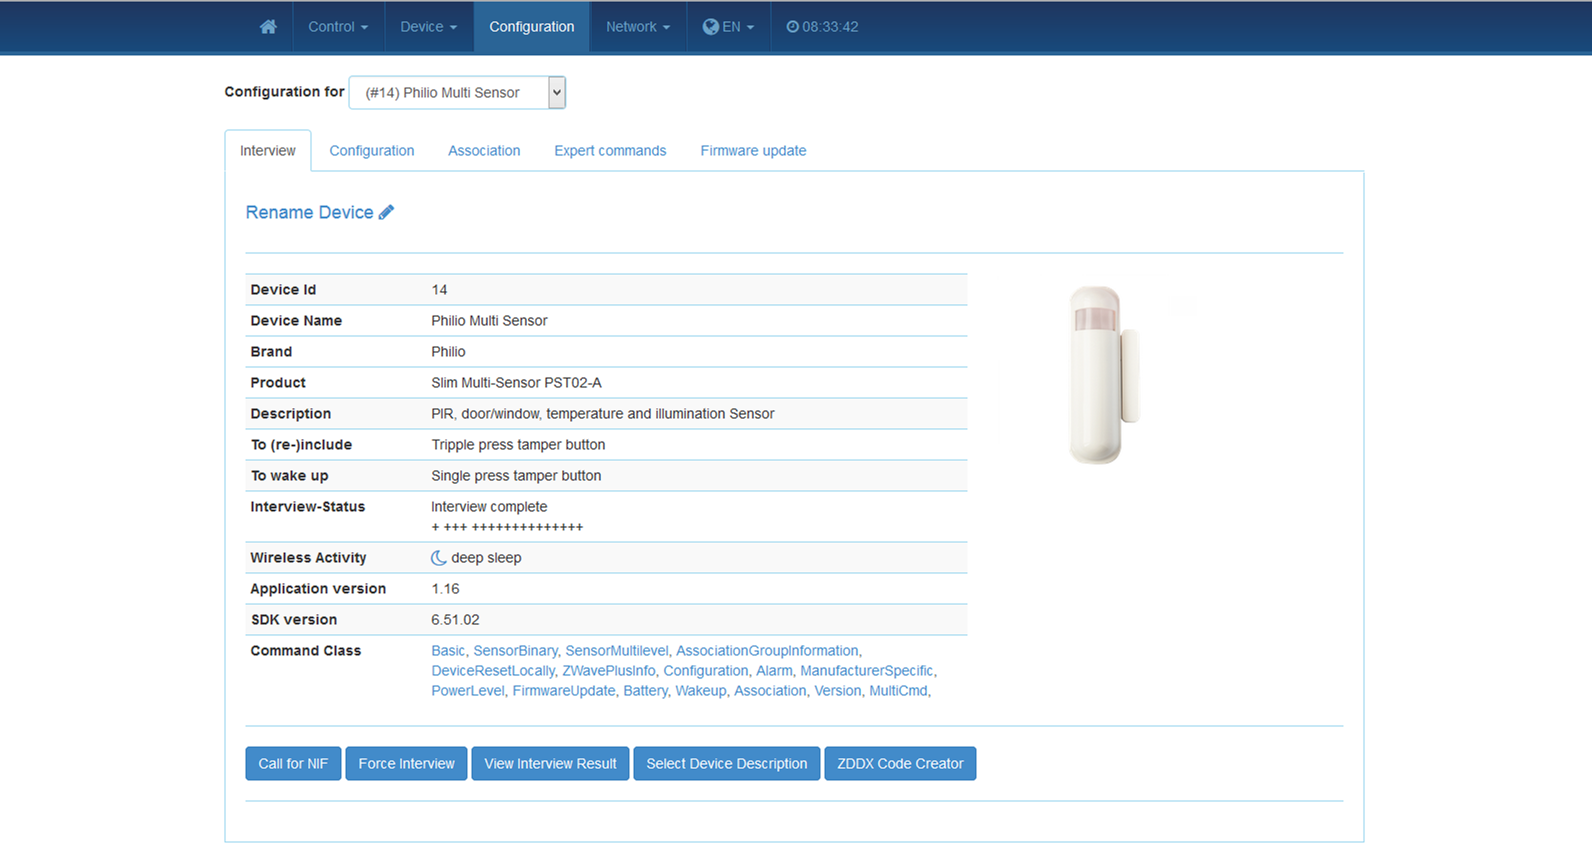
\includegraphics[width=0.9\textwidth]{img/Sensorevaluation/PhilioConf1.png}
	\caption{Übersichtsseite des Philio 4-in-1 Multisensors}
	\label{fig:sensorenPhilioConf1}
\end{figure}

Der Z-Way Server erstellt automatisiert eine Übersichtsseite, nachdem der Sensor erfolgreich hinzugefügt wurde. In diesem Reiter besteht die Möglichkeit, das Gerät umzubenennen, den Netzwerkstatus abzurufen und die aktuelle Sensor-Version abzufragen. Im Reiter „Configuration“ findet man alle Einstellungsmöglichkeiten die der Sensor bietet. In der nachfolgenden Tabelle (\prettyref{tab:PhilioConf}) sind die wichtigsten Konfigurationsoptionen aufgelistet.


\begin{longtabu} to \linewidth {
		>{\hsize=0.1\hsize}X
		>{\hsize=0.9\hsize}X
		>{\hsize=1.5\hsize}X 
		>{\hsize=1.5\hsize}X
		% sum=4.0\hsize for 4 columns
	}
	\hline
	\textbf{Nr}
			& \textbf{Name}
					& \textbf{Beschreibung}
							& \textbf{Werte} \\
	\hline
	2	
			& Grundeinstellung 
					& Setzt den Standardwert, um das Licht einzuschalten
							& -1 \textrightarrow{ }einschalten \newline 1 – 99 \textrightarrow{ }Dimmerintensität \\
	\hline
	3	
			& Sensitivität Bewegungsmelder 
					& Festlegen der Bewegungserkennungsintensität
							& 0 \textrightarrow{ }keine Bewegungserkennung \newline
							1 – 99 \textrightarrow{ }1 ist niedrigste Sensitivität, 99 die höchste \\
	\hline
	4	
			& Lichtschwellwert 
					& Festlegen des Beleuchtungsschwellwertes, um das Licht einzuschalten. Wenn das Event auslöst und die Umgebung dunkler ist, als der Schwellwert, geht das Licht an 
							& 1 – 99 \textrightarrow{ }1 ist dunkel, 99 ist hellster Wert \newline
							100 \textrightarrow{ }Lichterkennung deaktiviert \newline
							0 \textrightarrow{ }Lichterkennung deaktiviert und das Licht wird nie angeschaltet \\
	\hline
	5	
			& Betriebsmodus 
					& Bit 0 und Bit 1 werden freigeschaltet, sobald der PID-Schalter auf Programmmodus umgeschaltet wurde
					%todo wirklich PID?
							& (Bit) 0 \textrightarrow{ }Sicherheitsmodus \newline
							(Bit) 1 \textrightarrow{ }Testmodus \newline
							(Bit) 2 \textrightarrow{ }Fenster-/Türsensor deaktiviert \newline
							(Bit) 3 \textrightarrow{ }0 für Fahrenheit, 1 für Celsius \newline
							(Bit) 4 \textrightarrow{ }deaktiviere Lichtwertübergabe bei Auslösen des Events \newline
							(Bit) 5 \textrightarrow{ }deaktiviere Temperaturwertübergabe bei Auslösen des Events
							 \\
	\hline
	6	
			& Multisensor Funktionsschalter
					& Setzt den Standardwert, um das Licht einzuschalten \newline
							& (Bit) 0 \textrightarrow{ }deaktiviere integrierte Beleuchtung \newline
							(Bit) 1 \textrightarrow{ }deaktiviere integrierte Bewegungsmelder-Beleuchtung \newline
							(Bit) 2 \textrightarrow{ }deaktiviere Bewegungsmelder \newline
							(Bit) 3 \textrightarrow{ }wenn Bit 2 0 ist (aktiviert), ist das Gerät dann im selben Raum installiert? 0 = gleicher Raum (Standard), 1 = anderer Raum \newline
							(Bit) 4 \textrightarrow{ }deaktiviere die Verzögerung von 5 Sekunden beim Licht ausschalten, wenn Tür/Fenster geschlossen wurden \newline
							(Bit) 5 \textrightarrow{ }deaktiviere automatisches Licht ausschalten, nachdem Fenster/Tür geöffnet wurden und das Licht anging (keine Verwendung, wenn Bit 2 = 0) \newline
							(Bit) 6 \textrightarrow{ }Aktivere Temperaturaufzeichnung. Temperaturreport alle 64 Sekunden, wenn Veränderung von 3 Grad Fahrenheit und Überschreitung von 140 Grad Fahrenheit \\
	\hline
	8	
			& Bewegungsmelder, erneute Entdeckungszeit
					& Setzen der nächsten Entdeckungszeit, wenn ein Objekt entdeckt wurde und sich das Gerät im Sicherheitsmodus befindet
							& 3 – 127 \textrightarrow{ }Eingegebener Wert mal 8 Sekunden entspricht dem Zeitwert. \newline
							Minimale Zeit beträgt 24 Sekunden. \\
	\hline
	9	
			& Abschaltlichtzeit
					& Setzen der Verzögerungszeit um das Licht wieder auszuschalten, wenn der Bewegungsmelder nicht ausgelöst hat und nachdem das Licht angeschaltet wurde
							& 4 – 127 \textrightarrow{ }Eingegebener Wert mal 8 Sekunden entspricht dem Zeitwert. \newline Minimale Zeit beträgt 32 Sekunden. \\
	\hline
	10	
			& Auto- Reportzeit der Batterielebensdauer
					& Intervallzeit für automatische Meldung über die Batterierestkapazität
							& 1 – 127 \textrightarrow{ }Eingegebener Wert mal 30 Minuten entspricht dem Zeitwert. \newline Minimale Zeit beträgt 30 Minuten. \\
	\hline
	11	
			& Auto-Reportzeit  des Fenster/Tür Status
					& Intervallzeit für automatische Meldung des Fenster/Tür Status
							& 1 – 127 \textrightarrow{ }Eingegebener Wert mal 30 Minuten entspricht dem Zeitwert. \newline Minimale Zeit beträgt 30 Minuten. \\
	\hline
	12	
			& Auto-Reportzeit der Beleuchtung
					& Intervallzeit für automatische Meldung des Beleuchtungsstatus
							& 1 – 127 \textrightarrow{ }Eingegebener Wert mal 30 Minuten entspricht dem Zeitwert. \newline Minimale Zeit beträgt 30 Minuten. \\
	\hline
	13	
			& Auto-Reportzeit der Temperatur
					& Intervallzeit für automatische Meldung der Temperatur
							& 1 – 127 \textrightarrow{ }Eingegebener Wert mal 30 Minuten entspricht dem Zeitwert. \newline Minimale Zeit beträgt 30 Minuten. \\
	\hline
\caption{Konfiguration des Philio Multisensor}
\label{tab:PhilioConf}
\end{longtabu}

\subsubsection{Praxistest}
Um das Gerät in das Netzwerk einbinden zu können, ist es für die erste Konfiguration nur notwendig, den Stromkreislauf mit der Batterie zu verbinden und schon verbindet sich das Gerät innerhalb von 5 Sekunden automatisch mit dem Z-Wave-Netzwerk, wenn sich der Controller im "`Inclusion Mode"' befindet. Wenn man zu einem späteren Zeitpunkt eine Integration in das Netzwerk wünscht, genügt es, den Manipulationsschutzschalters auf der Rückseite drei Mal zu drücken. Ein einmaliges Drücken des erwähnten Schalters, hat eine Wake-up-Funktion zur Folge.

In manchen Fällen besteht nach Recherche allerdings die Möglichkeit, dass nach dem Inkludieren keine Funktion angezeigt wird. Um dem Abhilfe zu schaffen, wurde die nachfolgende Anleitung erstellt.

Z-Wave verfügt über die Möglichkeit, Geräte als "`secure"' in das Z-Wave-Netzwerk zu inkludieren. Dabei erfolgt die Kommunikation zwischen dem Sensor und dem Gateway verschlüsselt. Allerdings ist es in diesem Falle möglich, dass der Philio-Multisensor keine Zustandsänderungen an das Gateway sendet. In diesem Falle muss man die Experten-Oberfläche des Z-Way-Servers öffnen (\prettyref{fig:sensorenPhilioConf2}).

\begin{figure}[h!]
	\centering
	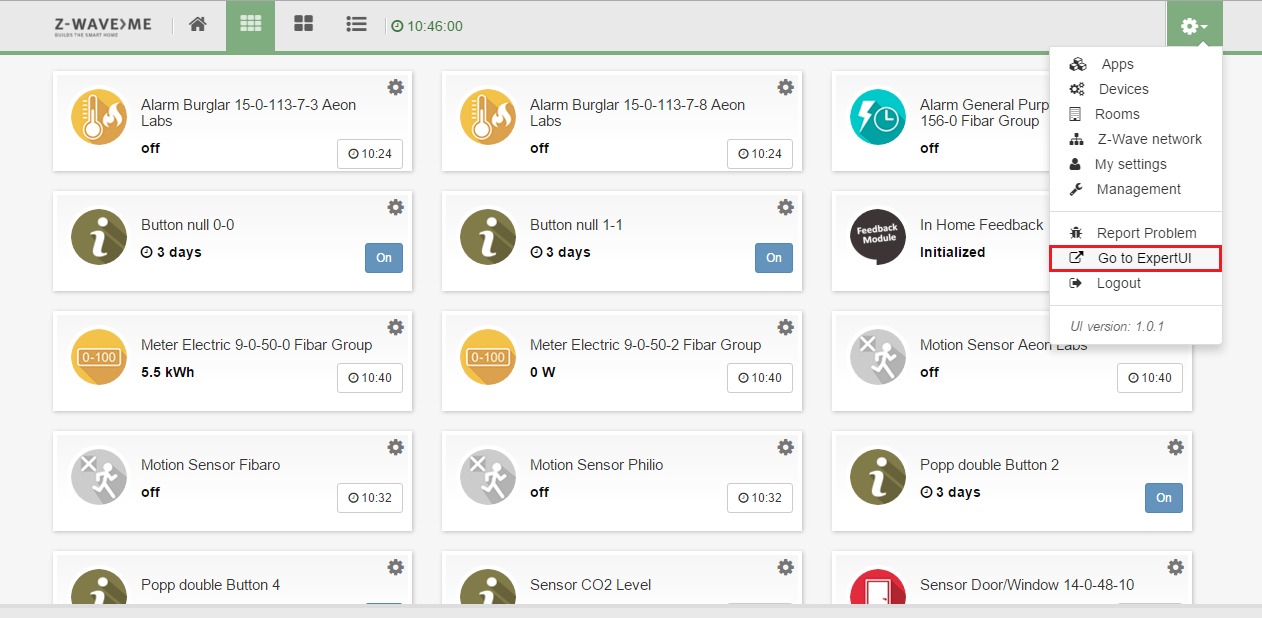
\includegraphics[width=0.9\textwidth]{img/Sensorevaluation/PhilioConf2.png}
	\caption{Oberfläche des Z-Way-Servers}
	\label{fig:sensorenPhilioConf2}
\end{figure}

Auf der Experten-Oberfläche wählt man anschließend den Menüpunkt \textbf{Network} und darunter den Menüpunkt \textbf{Control} (\prettyref{fig:sensorenPhilioConf3}).

\begin{figure}[h!]
	\centering
	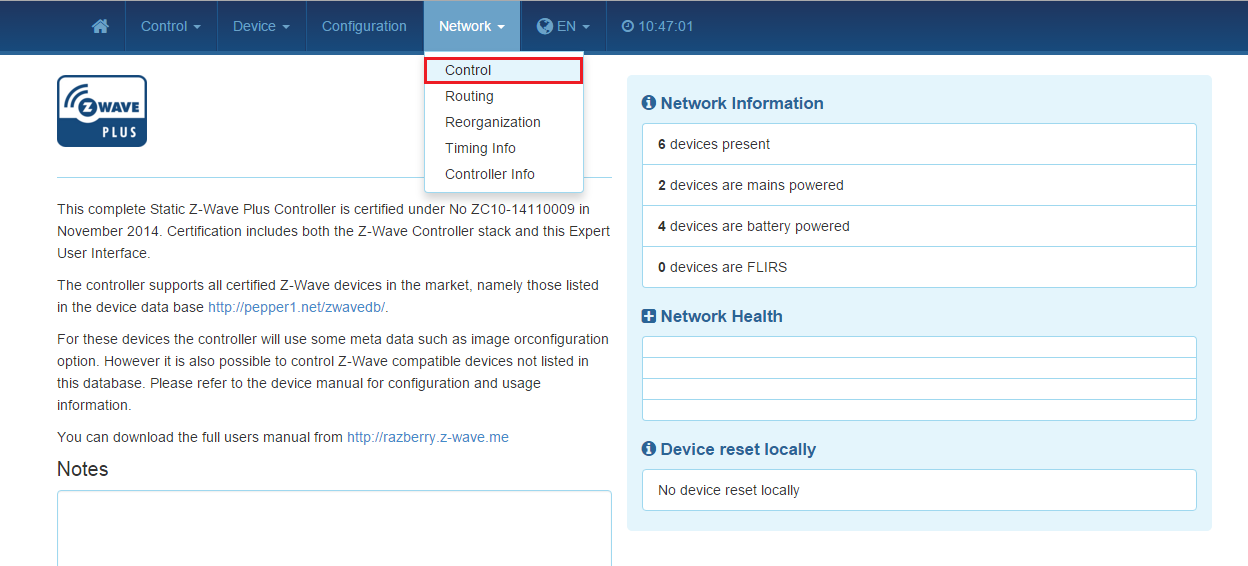
\includegraphics[width=0.9\textwidth]{img/Sensorevaluation/PhilioConf3.png}
	\caption{Experten-Oberfläche}
	\label{fig:sensorenPhilioConf3}
\end{figure}

An dieser Stelle hat man die Möglichkeit, den Inkludiermodus von „secure“ zu „unsecure“ zu ändern (1.). Anschließend muss man den „Start Inclusion“-Button drücken (2.), um das Inkludieren zu beginnen (\prettyref{fig:sensorenPhilioConf4}). 

\begin{figure}[h!]
	\centering
	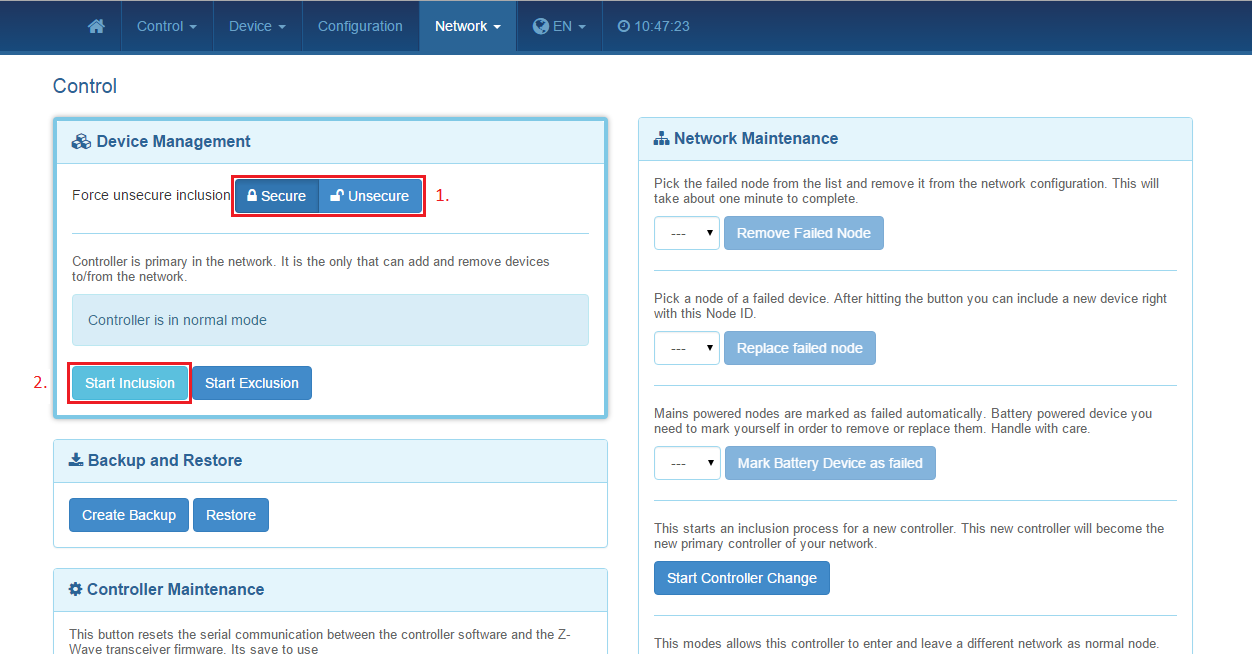
\includegraphics[width=0.9\textwidth]{img/Sensorevaluation/PhilioConf4.png}
	\caption{Auswahl des Inkludiermodus}
	\label{fig:sensorenPhilioConf4}
\end{figure}

Wenn man nun die kleine Schalter-Lasche des Sensors 3x hintereinander (innerhalb von 1,5 Sekunden) betätigt, sollte der Multisensor erfolgreich in das Z-Way-Netzwerk integriert worden sein. Auf der Smart Home Benutzeroberfläche werden die Elemente automatisch generiert, welche die Funktionen des Philio-Multisensors darstellen.

\section{Gefahrenquellenabschaltung}

\section{Alarmanlage}

\newpage
\section{Feedback-Mechanismen}
Bisher wurde davon ausgegangen, dass für ein leistungsfähiges intelligentes Haus Feedback-Möglichkeiten vorhanden sein sollen. Orientiert man sich an den Fähigkeiten des Menschen, sind dies das menschliche Sehen, Hören, Fühlen , Bewegen, Riechen und Schmecken. Insbesondere das Sehen, Hören und Bewegen sind für Feedbacks von Bedeutung. Als Möglichkeit für eine Rückmeldung stehen Displays, akustische Systeme und Gesten zur Verfügung. Um nun geeignete Reaktionen zu erwirken, bedarf es einer in Grenzen leistungsfähigen Systemintelligenz. Hierdurch wird die Repräsentation durch mögliche Interaktionen mit dem Smart Home möglich und hilft, den Eindruck von \glqq Intelligenz\grqq{} zu vermitteln. Auch dies ist eine wichtige Eigenschaft für die flexible Anpassungsfähigkeit an die vom Nutzer vorgegebenen Aufgabenstellungen. Die Anforderungen richten sich gleichermaßen, sowohl an sensorische Fähigkeiten als auch an die Fähigkeit, Daten von Sensoren in Erkenntnisse zu transformieren und daraus Strategien und Konzepte zu entwickeln. Methoden zur Wahrnehmung der Umwelt sowie zur Kommunikation mit dieser, stehen seit Jahren im Fokus der Forschung.\\
Im folgenden werden einige Forschungsarbeiten vorgestellt die im Laufe der Ausarbeitung entdeckt wurden. Unter anderem werden Möglichkeiten beschrieben die später in dem Projekt als Feedback eingesetzt werden können. Es werden auch schon vorhandene Lösungen auf dem Markt vorgestellt, die übernommen werden können. Es soll auch der Kostenfaktor berücksichtigt werden, da es nicht bekannt ist, ob die teuren Lösungen in dem Projekt eingesetzt werden können.\\
Weiter unten werden am Markt vorhandene Systeme und Lösungen kurz aufgelistet.\\

\subsection{Steuermechanismen auf Basis von Akustik}
\acrfull{tts} wandelt Fließtext in eine akustische Sprachausgaben um. Diese Technologie wird von den meisten Sprachmechanismen benutzt.

\begin{figure}[h!]
	\centering
	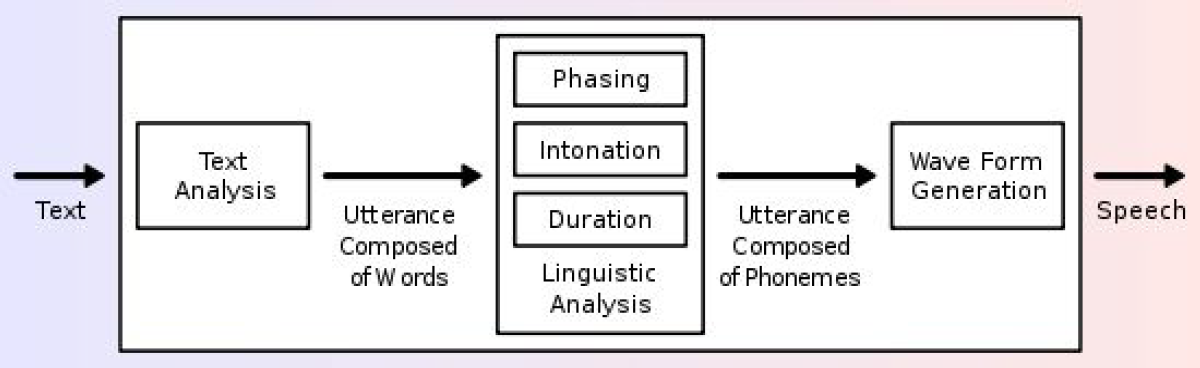
\includegraphics[width=0.9\textwidth]{img/Feedback-Mechanismen/TTS.png}
	\caption{\gls{tts}}
	\label{fig:feedbackTTS}
\end{figure}

Der Einsatz von sprach-gesteuerten Systemen hat bereits auf verschiedensten Gebieten, mehr oder weniger erfolgreich Einzug gehalten.

\subsubsection{IVEE}
Die nachfolgenden Ausführungen beziehen sich auf die Onlinequelle \glqq Deine Sprachsteuerung für dein SmartHome\grqq\footnote{\url{http://www.siio.de/connected-home/ivee-deine-sprachsteuerung-fuer-dein-smarthome/}}.

\begin{itemize}
\item Kosten: 200\$
\end{itemize}

\noindent
Bei ivee handelt es sich um eine cloudbasierte Sprachsteuerung für das Smart Home, bei der vom Marktstart an bereits diverse Hersteller angebunden sind. Hervorzuheben sind hier Belkin WeMo, Philips Hue, Logitech Harmony \& Google Nest sowie Z-Wave. Zu den genannten Anbietern werden kontinuierlich Neue dazu kommen. Nützlich könnten hier zum Beispiel eine Anbindung durch \gls{iftttg} oder an Google sein. Mit \gls{iftttg} könnten mit einem Schlag eine Vielzahl weiterer Dienste angebunden werden und mit der Anbindung an Google könnte man sich neue Mails oder Kalendereinträge vorlesen lassen. Die Installation und Steuerung von ivee ist auch für wenig technisch versierte Personen einfach umzusetzen. Die Sprachsteuerung ivee muss dazu nur an den Strom angeschlossen – und ins heimische WLAN integriert werden. Mit der dazugehörigen Smartphone App kann ivee beigebracht werden, welche Geräte im Haushalt verfügbar sind. Auch die Steuerung ist denkbar einfach:

\begin{enumerate}
\item Sag einfach \glqq Okay ivee\grqq{} zum Aufwecken. Der eingebaute, farbige LED-Ring wird blau und das System ist bereit für den Sprachbefehl.
\item Dann einfach das Kommando sagen oder die Frage stellen. Zum Beispiel: \glqq Schalt den Fernseher ein\grqq .
\item ivee schaltet den Fernseher an.\\
\end{enumerate}

Mit der iPhone-App können auch unterschiedliche Szenen angelegt werden, die zum Beispiel bei einem bestimmten Kommando die HUE-Leuchten dimmen, den Fernseher anschalten und die Raumtemperatur erhöhen. Alles möglich.

\begin{figure}[h!]
	\centering
	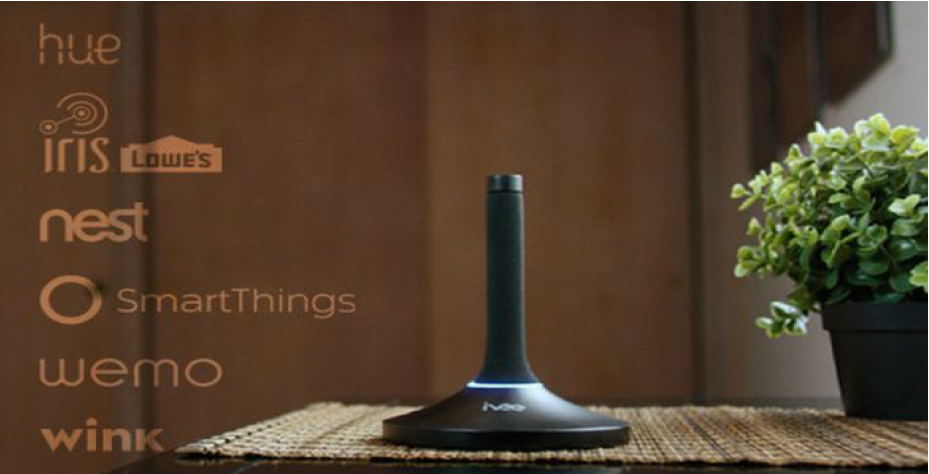
\includegraphics[width=0.9\textwidth]{img/Feedback-Mechanismen/IVEE.png}
	\caption{IVEE}
	\label{fig:feedbackIVEE}
\end{figure}

Art des Feedbacks: Es kann mit ivee Dialog ausgeführt werden, als Feedback erhält eine Person von ivee eine sprachliche Bestätigung zurück, die mittels eingebaute Mikrofone übermittelt wird, das die Aktion ausgeführt wurde.

\subsubsection{CastleOS Voice}
Die nachfolgenden Ausführungen beziehen sich auf die Onlinequelle \glqq CastleOS Voice-Controlled Home Automation Software for INSTEON, Z-Wave, WeMo, and More\grqq\footnote{\url{http://www.smarthome.com/castleos-voice-controlled-home-automation-software-for-insteon-z-wave-wemo-and-more.html}}.

\begin{itemize}
\item Kosten: 200\$
\end{itemize}

\noindent
CastleOS Voice-Controlled Home Automation Betriebssystem für INSTEON, X10, Z-Wave, UPB, LightwaveRF, WeMo, Nest, Sonos, Plex, XBMC, MediaBrowser3, DirecTV. Es ist kompatibel mit folgenden Smart Home Geräten wie Aeon Labs, Yale, Phillips, Honeywell, GE, Leviton, Sonos. CastleOS verwendet eine einzigartige Dual-Gerätesteuerung, die einfache Sprachbefehle durch eine Kinect oder CastleOS Web- und Mobile-Anwendung auf jedem iOS und Android Gerät akzeptiert. Befehle werden von der Kinect oder Web- und Mobile-Anwendung auf einen Windows PC, der mit einer unbegrenzten Anzahl von verbundenen Heimautomatisierungsgeräte, wie INSTEON, Z-Wave, UPB, X10 oder WeMo weitergeleitet. CastleOS kann nicht nur auf Sprachbefehle reagieren, sondern auch mit dem Ton Bestätigungen und Antworten auf Fragen und Befehle zu ausgeben. Kinect ermöglicht eine vollständige Kontrolle über ihr Zuhause mit einem präzisen und anspruchsvollen Spracherkennungssystem. Ihr Haus wird 24/7 ohne Störungen durch laute Musik, Filme, TV und andere Geräusche überwacht. Es gibt keine Begrenzung für die Anzahl der Kinect-Geräte die angeschlossen werden können aber zusätzliche Kinects erhöhen den Standard Übertragungsbereich um bis zu 10 Meter. Es kann auch mittels Mobil- bzw. Webapp gesteuert werden, falls keine Kinect vorhanden ist.

\begin{table}[H]
	\begin{tabularx}{\textwidth}{
			>{\hsize=0.5\hsize}X 
			>{\hsize=1.5\hsize}X
			% sum=2.0\hsize for 2 columns
		}
		\hline
		Betriebssystem	
		& Windows 7 oder neuer \\
		\hline 
		Z-Wave
		& Aeon Labs Z-Stick \\
		\hline
	\end{tabularx}
	\caption{Systemanforderungen: CastleOS}
\end{table}

\begin{table}[H]
	\begin{tabularx}{\textwidth}{
			>{\hsize=0.5\hsize}X 
			>{\hsize=1.5\hsize}X
			% sum=2.0\hsize for 2 columns
		}
		\hline
		Kompatibilität	
		& INSTEON, Z-Wave, UPB, WeMo \\
		\hline 
		Sprachsteuerung
		& mit Kinect und Kinect Voice Interface, Reichweite: 10,66 m, natürliche Sprachbefehle \\
		\hline 
		Gerätegruppierung
		& Szene, Gruppe \\
		\hline
	\end{tabularx}
	\caption{Features: CastleOS}
\end{table}

Die Änderungen, die mit Version CastleOS 2.0 erscheinen sollen, werden die Erstellung von virtuellen Geräten und Protokollen ermöglichen. Auf diese Weise können beliebige HTTP-Aufrufe ausgeführt werden. Der endgültige Termin ist nicht festgelegt, laut  Q\&A auf der offiziellen Webseite wird es noch dauern bis es in die Produktion geht.

\glqq The REST API was added a few months ago to support Android App development. To discover the services, you can use any web service explorer and point it to CastleOS on your machine: \url{http://localhost/CastleOS/service?wsdl}. You can also put that address in your web browser to see the raw XML if you'd like. The Custom Scripting as an Action is in testing now, and will be in the next release.\grqq

\subsubsection{Amazon Echo}
Die nachfolgenden Ausführungen beziehen sich auf die Onlinequelle \glqq Amazon hört und spricht ins Wohnzimmer\grqq\footnote{\url{http://www.golem.de/news/amazon-echo-amazon-hoert-und-spricht-ins-wohnzimmer-1411-110371.html}}

\begin{itemize}
\item Kosten: 179,99\$
\end{itemize}

\noindent
Der Echo kann jetzt auch Belkin WeMo und Philips Hue Produkte steuern. Amazon Echo sieht aus wie ein kleiner Bluetooth-Lautsprecher, der aber viel mehr kann als nur Musik abzuspielen. Das Gerät ist per WLAN mit dem Internet verbunden und besitzt sieben Mikrofone, mit denen es jedes Gespräch im Raum registrieren kann. Eine Fernbedienung mit eingebauten Mikrofonen, welche benutzt werden kann, wenn der Hub außer Reichweite ist, steht zur Verfügung.

\begin{table}[H]
	\begin{tabularx}{\textwidth}{
			>{\hsize=0.5\hsize}X 
			>{\hsize=1.5\hsize}X
			% sum=2.0\hsize for 2 columns
		}
		\hline
		WiFi	
		& zur Einbindung in das Heimnetz \\
		\hline 
	 	Bluetooth
		& Audiostreaming für Amazon Echo Mobilgeräte, Fernbedienung \\
		\hline 
	 	Systemanforderungen
		& Zugriff über Mobile-App oder Weboberfläche \\
		\hline
	\end{tabularx}
	\caption{Spezifikation: Amazon Echo}
\end{table}

\begin{figure}[h!]
	\centering
	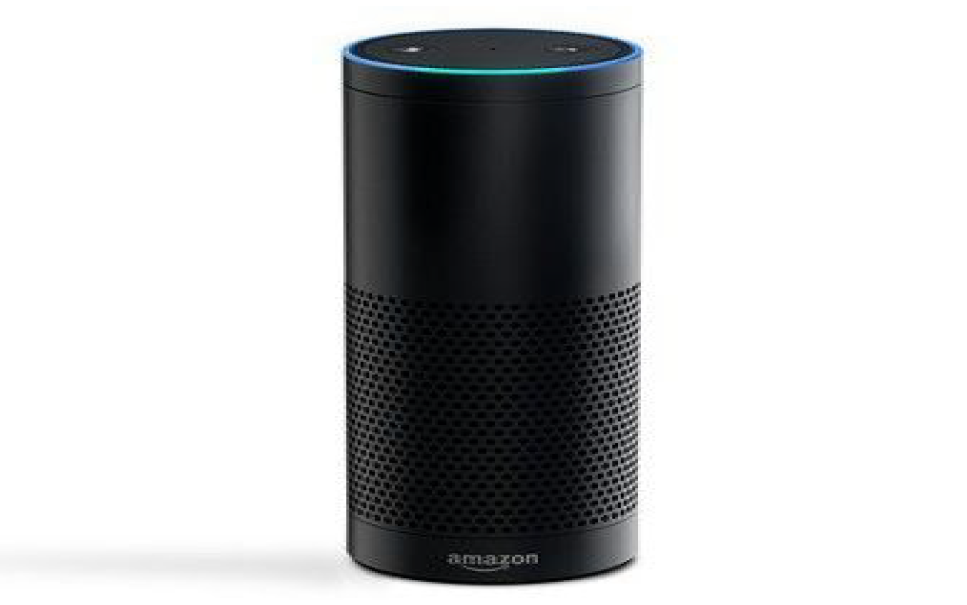
\includegraphics[width=0.9\textwidth]{img/Feedback-Mechanismen/AmazonEcho.png}
	\caption{Amazon Echo}
	\label{fig:feedbackAmazonEcho}
\end{figure}

Eine Anleitung zur Anbindung an Z-Wave ist unter \url{http://www.myzwave.net/index.php/adding-voice-control-to-vera-z-wave-systems-using-amazon-echo/2/} zu finden.

Die nachfolgenden Ausführung beziehen sich auf die Onlinequelle \glqq Amazon\grqq\footnote{\url{http://www.amazon.com/dp/B00X4WHP5E}} und \glqq Smart Home - Home Automation Superstore\grqq \footnote{\url{http://www.smarthome.com/amazon-echo-alexa.html}}.

Amazon Echo kommuniziert visuell mit dem Benutzer über sein Status mit Hilfe einer farbigen Beleuchtung ganz oben und unten:

\begin{figure}[h!]
	\centering
	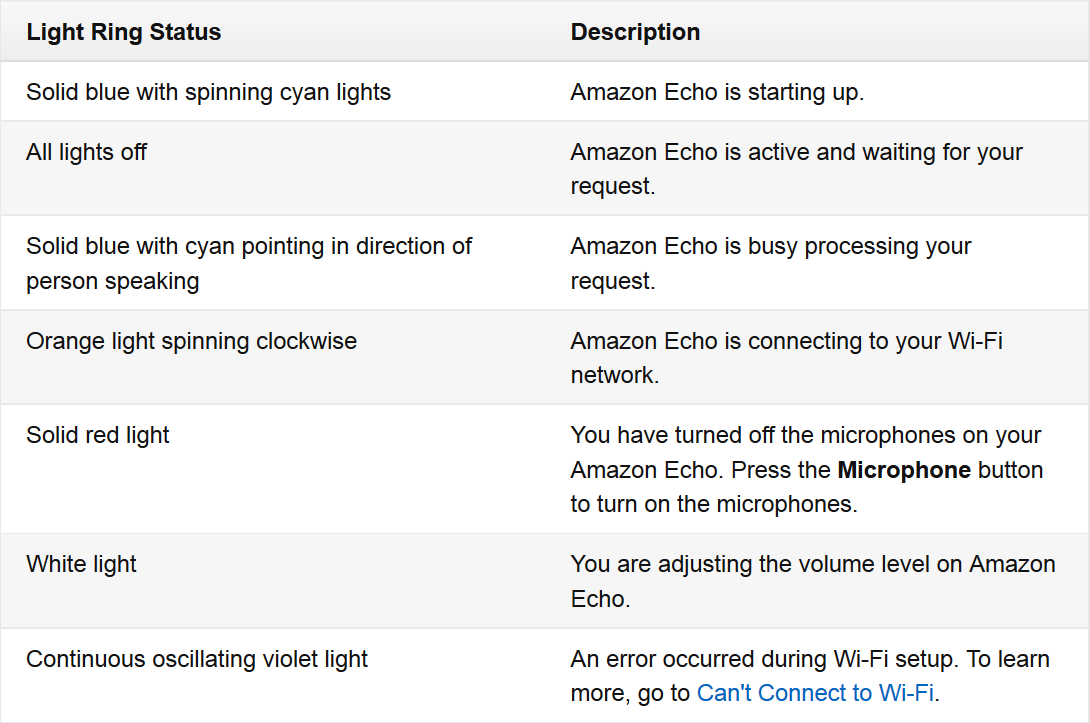
\includegraphics[width=0.9\textwidth]{img/Feedback-Mechanismen/AmazonEchoLight.png}
	\caption{Amazon Echo - Beleuchtung}
	\label{fig:feedbackAmazonEchoLights}
\end{figure}

Wenn ein Befehl ausgelöst wurde, wird Amazon Echo mit \glqq OK\grqq{} zurück antworten, wenn z.B gesagt wurde \glqq Licht an\grqq , wird \glqq OK\grqq{} ausgegeben.

How to control Z-Wave devices with amazon echo via SmartThings hub (\url{http://misterhouse.blogspot.de/2015/10/amazon-echo-smartthings-howto.html})

Die Z-Wave Geräte können von Amazon Echo mithilfe von SmartThings Hub gesteuert werden. In
Amazon App Einstellungen wird Amazon zu Smartthings verlinkt, und danach können alle Geräte
identifiziert werden. Nachdem die Geräteidentifizierung abgeschlossen ist, kann der Nutzer seine Geräte schon per Amazon Echo steuern.

Mit Amazon-Echo-ha-bridge wird ein Hue Hub emuliert, und es können vom Benutzer virtuell erstellte Geräte von diesem Hub identifiziert werden. Diese Geräte können konfiguriert werden um HTTP Rest Befehle zu den anderen Geräten im Haus senden und diese steuern zu können.

HowTo Amazon-Echo-Bridge (\url{https://github.com/armzilla/amazon-echo-ha-bridge})

\noindent
\glqq HowTo: Using Echo to control SmartThings:
Amazon-echo-ha-bridge which is a Java application that emulates a Hue/WeMo hub. The user can
create virtual \glqq lights\grqq{} that Echo will discover using it's native Hue/WeMo support. You can configure the \glqq lights\grqq{} to send HTTP REST commands to other systems in your house. You can say \glqq turn on the <xxx>\grqq , \glqq turn off the <yyy>\grqq , or \glqq set the <zzz> to 50\%\grqq{} (or whatever value). These are utilizing the on/off/dim verbs that Echo understands for light controls, so it works best for activities that would make sense in this sort of sentence. \glqq Alexa, set the thermostat to 78 percent\grqq{} might be ok for setting the temperature.\grqq

\subsubsection{Homey}
Die nachfolgenden Ausführungen beziehen sich auf die Onlinequelle \glqq Homey, preheat the oven! This orb lets you control your house with your voice\grqq\footnote{\url{http://www.digitaltrends.com/home/homey-adds-jarvis-style-voice-control-practically-everything-house/}}

\begin{itemize}
\item Kosten: 299,00€
\end{itemize}

\noindent
Homey unterstützt auch Dinge wie NFC, nRF24L01 + und Infrarot, sowie Z-Wave, ZigBee,
Bluetooth und WiFi. Es wird verwendet, um TV, nicht vernetzte Soundsysteme zu steuern und sogar
Computer. Der Vorteil ist das Homey eine natürliche Sprache versteht. Es sollen keine Befehle in einer bestimmten Reihenfolge ausgesprochen werden, um mit dem Homey zu interagieren. Homey ist mit einem \textit{natural language} Prozessor ausgestattet und versteht die Kurzbefehlen die zur Hausautomatisierung ausgerichtet sind. Es können folgende Befehle wie z.B. \glqq Heizung an\grqq , \glqq Tür zu\grqq{} oder \glqq Licht an\grqq{} ausgesprochen werden und es wird vom System verstanden. Homey ist mehrsprachig, u.a Deutsch.

\begin{figure}[h!]
	\centering
	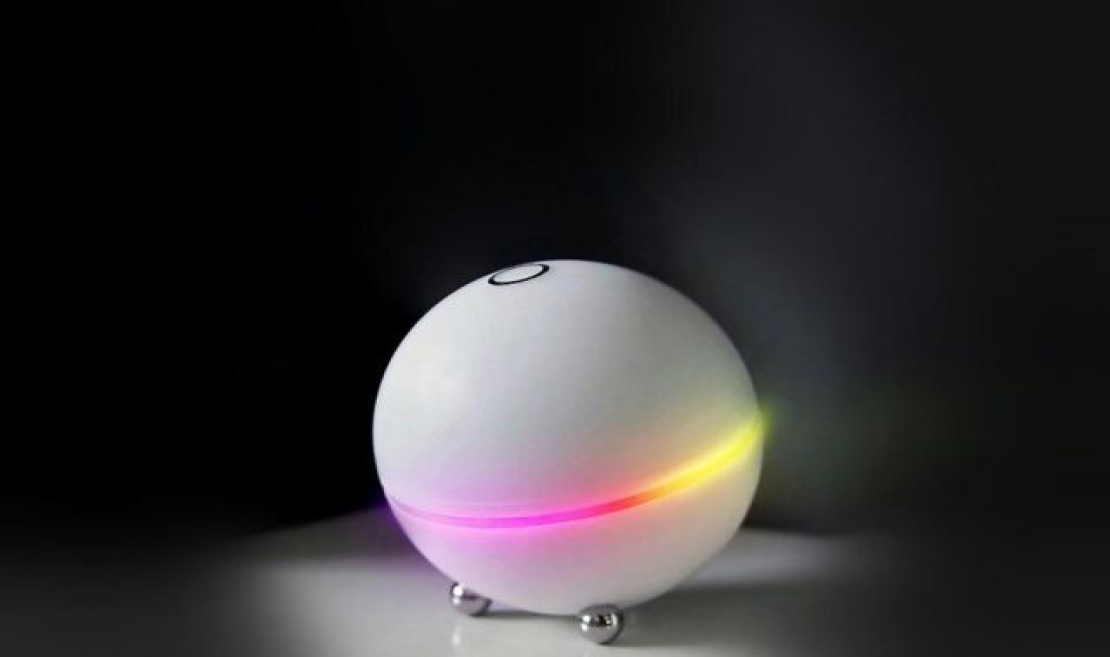
\includegraphics[width=0.9\textwidth]{img/Feedback-Mechanismen/Homey.png}
	\caption{Homey}
	\label{fig:feedbackHomey}
\end{figure}

Mit REST API, kann der Benutzer mit Homey interagieren und von außen HTTP Anfragen senden
um die Geräte zu steuern. Die Verwendung ist unter \url{https://developers.athom.com/api/#} erklärt.

\subsubsection{EnBlink}
Die nachfolgenden Ausführungen beziehen sich auf die Onlinequellen \glqq Enblink dongle now lets you control smart home devices with voice commands\grqq\footnote{\url{http://www.digitaltrends.com/home/enblink-dongle-now-lets-control-smart-home-devices-voice-commands/}} und \glqq Smart Home - Home Automation Superstore\grqq\footnote{\url{http://www.smarthome.com/enblink-ss201-us-w-z-wave-usb-plug-in-controller.html}}.

\begin{itemize}
\item Kosten: 89,99\$
\end{itemize}

\noindent
Es handelt sich hierbei um einen kleine USB-Stick, der in jedes Google-TV-Gerät gesteckt werden kann und wandelt es in einen Hub, welcher das Haus steuert. Es funktioniert mit jedem Z-Wave-kompatiblen Gerät in ihrem Haus, das heißt, sie können es verwenden, um alles steuern zu können Lampen, Türschlösser, Sicherheitssensoren, Thermostate, und vieles mehr. EnBlink kann jedes Z-Wave-fähige Heimgerät von einer zentralen Stelle kontrollieren, das kann eine Wandplatte, Touchpad, PC, SmartTablet oder Smartphone sein.

\begin{figure}[h!]
	\centering
	
\includegraphics[width=0.4\textwidth]{img/Feedback-Mechanismen/EnBlink.png}
	\caption{EnBlink}
	\label{fig:feedbackEnBlink}
\end{figure}

\begin{table}[H]
	\begin{tabularx}{\textwidth}{
			>{\hsize=0.5\hsize}X 
			>{\hsize=1.5\hsize}X
			% sum=2.0\hsize for 2 columns
		}
		\hline
		Hersteller	
		& EnBlink \\
		\hline 
	 	Z-Wave Chip
		& ZW0301 \\
		\hline 
	 	Z-Wave Bibliothek
		& Serial API \\
		\hline 
	 	Basic Device Class
		& Z-Wave Controller \\
		\hline 
	 	Reichweite
		& ca. 30 m \\
		\hline 
	\end{tabularx}
	\caption{Spezifikation: Amazon Echo}
\end{table}

\subsubsection{HALBasic - Home Automation living}
Die nachfolgenden Ausführungen beziehen sich auf die Onlinequelle\footnote{\url{www.automatedliving.com/HALbasic.aspx}}

\begin{itemize}
\item Kosten: 19,99€
\end{itemize}

\noindent
Z-Wave compatible UI (PC Control)-Software HALBasic ermöglicht begrenzte Geräte im Hausnetz
durch PC Software zu steuern. HAL verbindet ein Mobiltelefon mit der Software auf PC durch die Telefonleitung. Nutzer benötigen einen Anruf für das Gerät die gesteuert werden soll tätigen und die Befehle senden, wie z.B Licht einschalten und wie lange. Alle Befehle werden durch den Computer gesteuert.

\begin{figure}[h!]
	\centering
	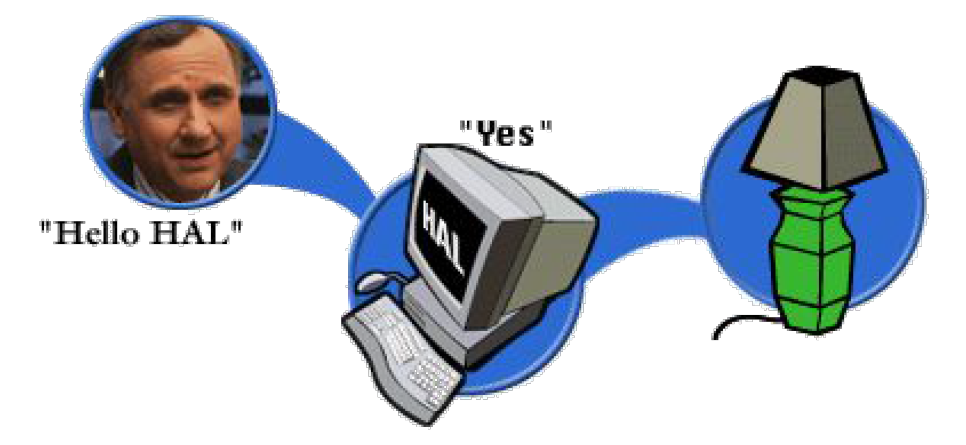
\includegraphics[width=0.7\textwidth]{img/Feedback-Mechanismen/HAL.png}
	\caption{HAL}
	\label{fig:feedbackHAL}
\end{figure}

\subsubsection{Z-Wave Fernbedienung}
Die nachfolgenden Ausführungen beziehen sich auf die Onlinequelle \glqq düwi Fernbedienung: Z-Wave Netzwerk ohne Smart Home Gateway einrichten\grqq\footnote{\url{siio.de/duewi-fernbedienung-z-wave-netzwerk-ohne-smart-home-gateway-einrichten/}}

\begin{itemize}
\item Kosten: 74,00€ bzw. 70,90€
\end{itemize}

\noindent
Mit Hilfe von folgenden Fernbedienungen können Geräte innerhalb des Heimnetzes gesteuert werden, die Anleitung zur Steuerung von Fernbedienung ist unter dem Link Schrittweise beschrieben.

\noindent
Z-Wave.Me: 

\begin{itemize}
\item Kosten: 74,00€
\item Steuerung mittels Z-Wave (z. B. Fibaro, Vera, Zipato) 
\item LED-Anzeige
\item 868,4 MHz Frequenz, für den Einsatz in 47 Ländern der CEPT (einschließlich der gesamten EU) plus China, Singapur, Südafrika, Vereinigte Arabische Emirate
\item unterstützt Ein/Aus-Schalter zum Bedienen der Geräte, Dimmen, Helligkeits-Steuerung für Beleuchtung und hoch/hinunter für motorbetriebene Geräte
\item für bis zu 10 Z-Wave-Gerätegruppen oder Szenen über 10 Paar Taste
\end{itemize}

\noindent
Düwi: 

\begin{itemize}
\item Kosten: 70,80€
\item Z-Wave Plus: nein 
\item Gerätetyp: Controller
\end{itemize}

\noindent
Unterschied Düwi und Z-Wave Ferndbedienung: 
Wenn es bereits eine Z-Wave Zentrale/Gateway im Einsatz ist, kann Düwi Fernbedienung auch in
Netzwerk verwendet werden.

\begin{itemize}
\item Düwi kann Stand-alone betrieben werden, Controller, kann nicht per Z-Wave Gateway konfiguriert werden
\item ZME kann nicht Stand-alone betrieben werden (kein Controller), Konfiguration von Assoziationen\&Szenen per Z-Wave Gateway möglich
\end{itemize}

\subsection{Steuermechanismen auf Basis von Gesten}

\subsubsection{OneCue}

Die nachfolgenden Ausführungen beziehen sich auf die Onlinequelle \glqq OneCue – Gestensteuerung für Ihr Smart Home\grqq\footnote{\url{http://smarthomewelt.de/onecue-gestensteuerung-smart-home/}}

\begin{itemize}
\item Kosten: 129,00\$
\end{itemize}

\noindent
eyeSights entwickelt wie das bereits von Microsofts Xbox bekannte Kinect-System nur auf Basis von Handgesten. Dazu ist das Gerät mit moderner Kamera-und Sensortechnik ausgestattet, die in der Lage ist, selbst kleinste Handbewegungen des Nutzers zu erkennen, korrekt zu interpretieren und für die mit OneCue verbundenen Geräte in die entsprechenden Befehle umzuwandeln. Die Steuerung für das Smart Home ist sehr intuitiv, das zeigt die Gestenerkennung mit der sich das TV-Gerät oder die Stereoanlage auf stumm schalten lässt: Klingelt beispielsweise das Telefon, reicht es den Zeigefinger wie bei einem \glqq Pssst!\grqq{} vor die geschlossenen Lippen zu führen um die Geräte vorübergehend in den Mute-Modus zu versetzen.

\begin{figure}[h!]
	\centering
	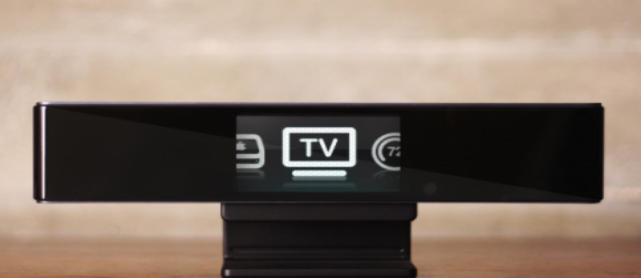
\includegraphics[width=0.7\textwidth]{img/Feedback-Mechanismen/OneCue.png}
	\caption{OneCue}
	\label{fig:feedbackOneCue}
\end{figure}

Das OneCue-Smart Home System ist ein kleiner schwarzer Box. Die Smart Home-Steuerung lässt sich jedoch theoretisch überall im Haus platzieren. Einzige Voraussetzung für eine reibungslose Funktion der Gestensteuerung ist eine direkte Sichtverbindung zwischen dem Nutzer und der OneCue-Empfangseinheit. Die Signalstärke des Gadgets reicht um auch Endgeräte in größeren Entfernungen zu bedienen. Bauliche Gegebenheiten im Smart Home können allerdings dafür Sorgen, dass WiFi- und Infrarot-Signale schon in wenigen Metern Entfernung nur noch schwach vorhanden sind. Für diesen Fall liefert eyeSight einen Repeater zur Signalverstärkung mit.

Für die Einrichtung können Nutzer wahlweise Bluetooth-fähiges Smartphone mit der in den App-Stores kostenlos verfügbaren OneCue-App (für iOS und Android) nutzen, oder auch PC/Laptop direkt mittels Micro-USB mit dem Gerät verbinden. Um für das Smart Home konzipierte Geräte wie das lernende Thermostat von Nest oder die vernetzten Leuchtmittel von Philips Hue mit Gesten über das OneCue bedienen zu können, müssen die bekannten WLAN Daten in der Konfiguration hinterlegt werden.

Mit welchem Gerät OneCue im Augenblick verbunden ist, lässt sich anhand großer Symbole von dem 3-Zoll-LC-Display auf der Front der Gestensteuerung ablesen. In dem System sind bereits Icons für verschiedenste Gerätetypen wie zum Beispiel Apple TV, Fernseher, Nest, Philips Hue, Stereoanlage, Set-Top-Box oder Blu-ray Player vorinstalliert.

Es wird ein API in weiteren Versionen entwickelt, die Entwicklern den Zugriff auf mehrere Geräte zu singlecue ermöglichen wird, das im Sommer 2016 veröffentlicht wird (\url{http://eyesight-tech.com/eyesight-technologies-announces-public-availability-of-singlecue-bringing-touch-free-gesture-control-to-your-home/}).

\subsubsection{Reemo}

Die nachfolgenden Ausführungen beziehen sich auf die Onlinequelle \glqq Reemo: Die Smart Home-Steuerung aus dem Handgelenk\grqq\footnote{\url{siio.de/reemo-die-smart-home-steuerung-aus-dem-handgelenk/}}

\begin{itemize}
\item Kosten: 299,00€
\end{itemize}

\begin{itemize}
\item 45 Gramm
\item funktioniert per Bluetooth
\item wasserdicht
\end{itemize}

\noindent
Dazu wird ein Receiver benötigt, welcher mit den gewünschten Smart Home-Produkten verbunden werden kann. Mit einer Geste (Reemo versteht insgesamt sechs verschiedene) können einzelne Aktionen, aber auch ganze Sequenzen ausgelöst werden.

\begin{figure}[h!]
	\centering
	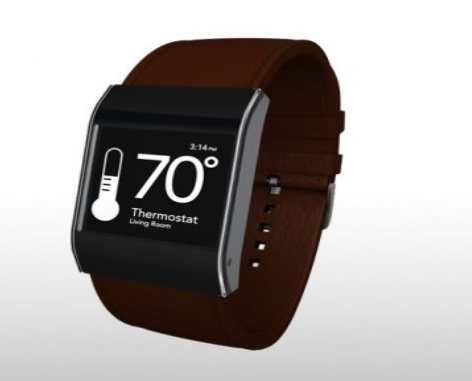
\includegraphics[width=0.7\textwidth]{img/Feedback-Mechanismen/Reemo.png}
	\caption{Reemo}
	\label{fig:feedbackReemo}
\end{figure}

Die Hersteller versprechen störungsfreie Verwendung mehrere Reemo's in einem Haus. Nehmen wir
an, Albert aktiviert mit Reemo den Nachtmodus (Licht aus, Alarm an, Türen zu etc.), das System
merkt aber, das Bertha in der Küche ist, dann bleibt dort das Licht an.

\noindent
Kompatibel mit:
\begin{itemize}
\item Logitech Harmony Ultimate Home
\item Philips Hue Lux/Tap, ZigBee lightbulbs
\item Thermostaten von Azela, Pearl, Computime, RTCOA
\end{itemize}

\noindent
Installation (\url{https://www.indiegogo.com/projects/control-your-world-with-reemo#/})

\begin{figure}[h!]
	\centering
	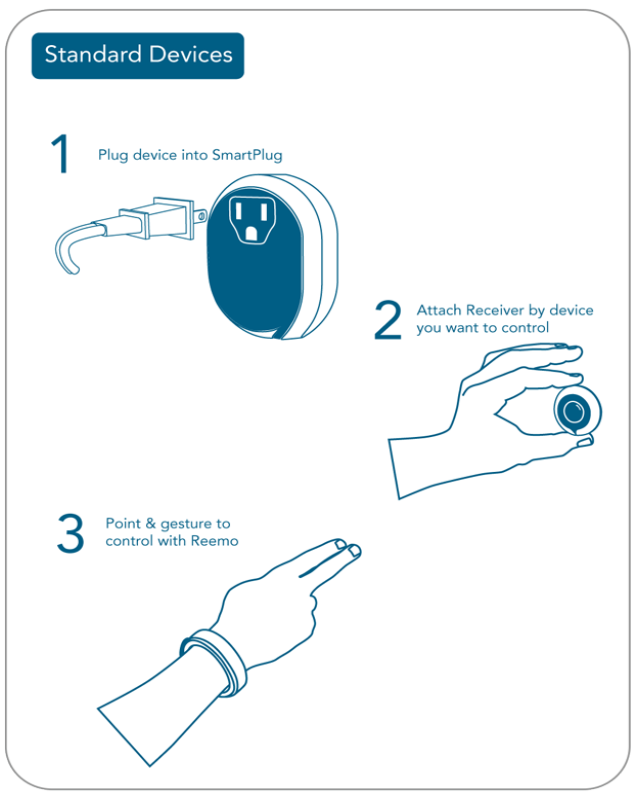
\includegraphics[width=0.7\textwidth]{img/Feedback-Mechanismen/ReemoInstallation1.png}
	\caption{Reemo Installation}
	\label{fig:feedbackReemoInstallation1}
\end{figure}

\begin{figure}[h!]
	\centering
	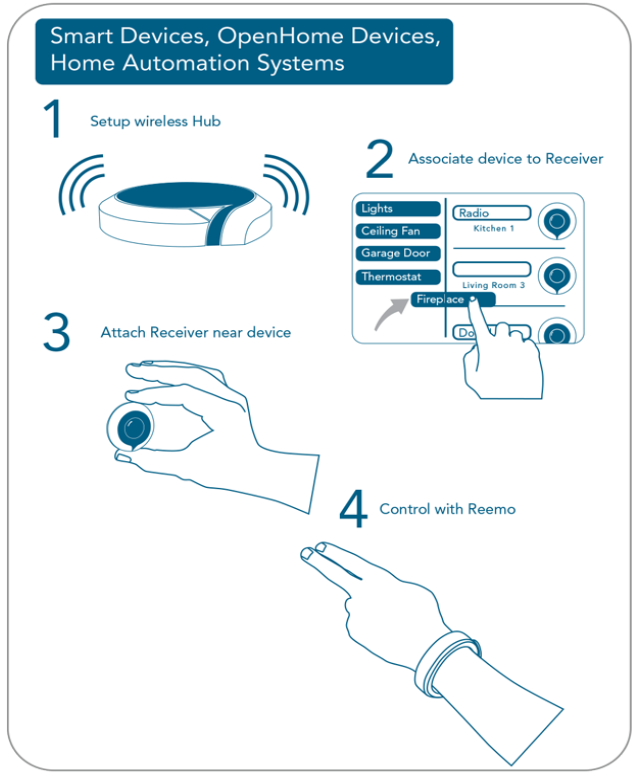
\includegraphics[width=0.7\textwidth]{img/Feedback-Mechanismen/ReemoInstallation2.png}
	\caption{Reemo Installation}
	\label{fig:feedbackReemoInstallation2}
\end{figure}

\noindent
Ein Feedback von Reemo wird den Benutzern über eine Vibration mitgeteilt. Wenn ein Benutzer auf eine Lampe zeigt und er einen Befehl starten will, wird am Reemo durch eine Vibration betätigt, dass das Gerät ausgewählt wurde. Danach kann Benutzer Gesten-Befehle ausführen.

\subsection{Studienergebnisse Sprach/Gestensteuerungssysteme}

\subsubsection{SCARS}

Die nachfolgenden Ausführungen beziehen sich auf die Onlinequelle \glqq HCI Aspects of Smart Environments\grqq\footnote{\url{http://www.uni-klu.ac.at/tewi/downloads/HASE10_Conference_Proceedings.pdf}}

\noindent
SCARS besteht im Wesentlichen aus fünf Hardwarekomponenten:

\begin{itemize}
\item EmpfängerEinheit
\item kabellose Mikrofone
\item Positionsbestimmungssystem
\item Lautsprecher
\item Softwareeinheit
\end{itemize}

\begin{figure}[h!]
	\centering
	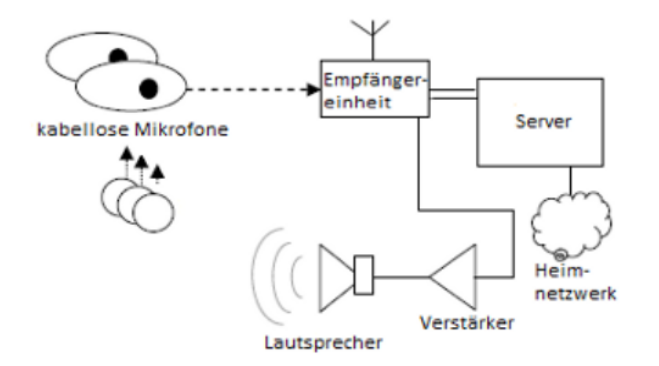
\includegraphics[width=0.4\textwidth]{img/Feedback-Mechanismen/SCARS.png}
	\caption{SCARS}
	\label{fig:feedbackSCARS}
\end{figure}

Alle Elemente wurden eigens für eine Smart Home Umgebung entworfen, um alle Erfordernisse so
gut wie möglich abzudecken. Auf dem Server läuft eine Spracherkennungssoftware von Philips, die
ca. 20 vordefinierte Befehle erkennen kann und in weiterer Folge die entsprechenden Aktionen
ausführt.
Wenn ein Audiosignal von einem Mikrofon empfangen wird, wird dieses von der Software verarbeitet, mit den vordefinierten Befehlen verglichen und falls eine Übereinstimmung gefunden wird, wird ein entsprechender Code an das SCARS-Softwaremodul weitergeleitet. Dieses wertet in weiterer Folge den Code aus und sendet die zutreffende Aufgabe an die Serversoftware (z.B. schalte das Licht im Wohnzimmer ein) und gibt dem Benutzer eine natürlichsprachliche Bestätigung zurück.
Dieses Audiofeedback wird durch einen \gls{tts} -Sprachgenerator erzeugt, der beliebige vordefinierte Zeichenketten wiedergeben kann.
Der Benutzer drückt den Knopf am Mikrofon und spricht ein definiertes Kommando wie zum Beispiel
\glqq schalte Licht ein\grqq{} und lässt den Knopf wieder los. Der Befehl wird daraufhin auf dem Server verarbeitet und die Lichter in dem Raum eingeschaltet, in dem sich der Benutzer gerade befindet. Abschließend gibt das System eine Bestätigung zurück.
Das System wurde von einer Gruppe von Studenten getestet, die generell positiv überrascht waren, wie einfach die Bedienung zu erlernen war. Auch die Erkennung der Sprachbefehle der Benutzer verschiedener Geschlechter und Altersgruppen war erfolgreich. Ein Manko sahen die Testpersonen in der Antwortzeit des Systems, weiter erachteten sie es als nicht sehr praktikabel, ständig ein Mikrofon bei sich tragen zu müssen. Ein weiteres Problem stellte die Verlässlichkeit des Positionierungssystems dar, da es oftmals lange Zeit brauchte bis die Software den richtigen Standort des Mikrofons definieren konnte bzw. auch falsche Lautsprecher angesprochen wurden, wenn sich die Personen nahe an einem angrenzenden Raum befanden.

\subsubsection{LOGOS}

Die nachfolgenden Ausführungen beziehen sich auf die Onlinequelle \glqq HCI Aspects of Smart Environments\grqq\footnote{\url{http://www.uni-klu.ac.at/tewi/downloads/HASE10_Conference_Proceedings.pdf}}

Ähnlich wie bei SCARS, setzt auch dieses System nicht nur rein auf eine Interaktionsmöglichkeit, sondern stellt insgesamt 3 verschiedene Möglichkeiten zur Verfügung. Es lässt sich entweder über eine Fernbedienung, eine PC-Tastatur oder über natürliche Sprache steuern. Das System bietet einen benutzerfreundlichen Zugang zu Informationen und Smart Home Geräten.

Die Funktionsweise des sprachgesteuerten Dialogsystems sieht wie folgt aus. Eine Reihe von Mikrofonen zeichnen das Sprachsignal der Benutzer auf, danach benutzt die Spracherkennungskomponente ein vordefiniertes akustisches Modell sowie ein Sprachmodell, um der \glqq Sprachverständniskomponente\grqq den erkannten Text zur Verfügung zu stellen. Diese interpretiert in weiterer Folge den Input und leitet die daraus resultierenden Informationen an den Dialogmanager weiter. Abhängig vom übergebenen Befehl, dem Gerätestatus und dem Dialogverlauf, generiert diese Komponente via \gls{tts} den Output, wodurch ein natürlichsprachlicher Dialog zwischen Benutzer und System zustande kommt. Der Application-Manager übernimmt die Synchronisation aller Daten zwischen dem Dialogmanager und den Smart Home Geräten indem er erhaltene Befehle entweder direkt ausführt oder diese wieder an den Dialogmanager zurückgibt. In zweiten Fall verarbeitet dieser die Anfrage und aktualisiert den Dialogfluss. Zusätzlich wird von dieser Komponente auch ein visuelles Feedback für die Benutzer generiert. Um die verschiedenen Einschränkungen die aus einer realistischen Umgebung resultieren zu bewältigen, wurde eine Anordnung von kommerziellen Mikrofonen installiert, die über insgesamt acht Sensoren verfügen. Dadurch wurde ein hohes Signal-Stör-Verhältnis erreicht, das heißt es konnte eine Vielzahl an Hintergrundgeräuschen sowie auch das Echo herausgefiltert werden und somit eine bessere Verständlichkeit des Sprechenden erreicht werden.

Hierbei handelt es sich um eine Spracherkennungskomponente, bei deren Entwicklung vor allem der Kostenfaktor eine wichtige Rolle spielte, da die derzeitigen sprachgesteuerten Systeme meist viel zu teuer sind, um eine weite Verbreitung zu finden. Die Komponente wurde anhand von echten Szenarien die im LOGOS System entwickelt wurden, getestet. Im Gegensatz zu Steuerungssystemen auf Basis von vordefinierten Befehlen, lässt sich diese Implementierung durch spontan gesprochene und nicht vorher definierte Befehle steuern. Die Implementierung beruht auf einer OpenSource Spracherkennung und einem kostengünstigen Mikrofon. Es wird kein Dialogsystem oder ein sprachliches Feedback verwendet, das einzige Feedback erhält der Benutzer vom Gerät selbst, wenn es in den von ihm gewünschten Zustand übergeht. Versuche zeigten dass durch diese Implementierung eine durchaus hohe Leistung erreicht werden kann. Der stabile Betrieb des Systems kombiniert mit seiner Wirtschaftlichkeit, machen es zu einer interessanten Alternative gegenüber anderen state-of-the-art Dialogsystemen.

Das System wurde von insgesamt 10 Testpersonen evaluiert, in dem sie spontane Befehle via tragbarem Mikrofon an das System richteten. Die Leistung der Spracherkennungskomponente und der Erfüllungsgrad der Aufgaben wurden unter verschiedenen Bedingungen untersucht. Einerseits wurden die Worterkennungsrate und andererseits der Erfüllungsgrad der Aufgaben gemessen. Insgesamt wurden vier verschiedene Experimente bezüglich der Umfeldbedingungen durchgeführt. Ein Experiment beruhte auf einem hochqualitativen Mikrofon mit Störsignalunterdrückung, die anderen drei Versuche wurden mit dem kostengünstigen tragbaren Mikrofon durchgeführt. Die Ergebnisse zeigten, dass die günstigen Mikrofone nur unwesentlich schlechter als das qualitativ hochwertige Mikrofon abschnitten. Des weiteren wurde in allen vier Szenarien ein Erfüllungsgrad der Aufgaben von 100 \% und eine durchschnittliche Worterkennungsrate von 95,67 \% erreicht. Diese höchst positiven Ergebnisse zeigen die Effektivität des Systems und dessen Robustheit in lärmintensiven Umgebungen.

\begin{figure}[h!]
	\centering
	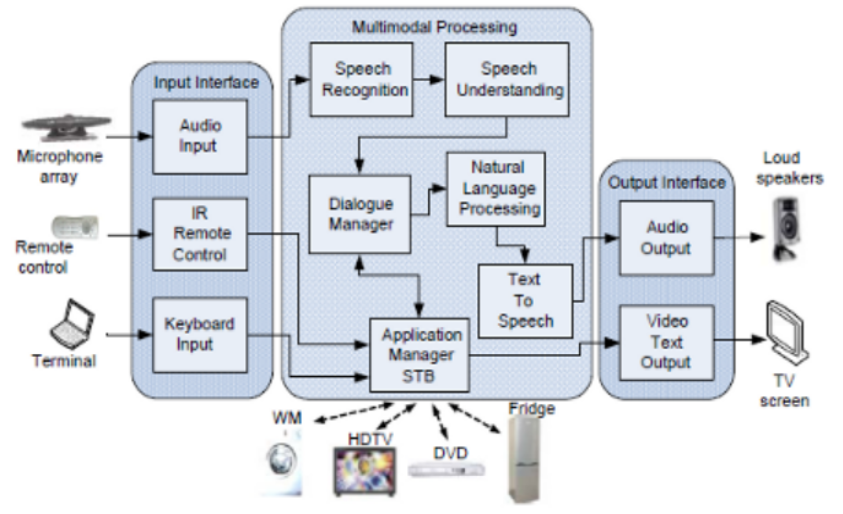
\includegraphics[width=0.7\textwidth]{img/Feedback-Mechanismen/LOGOS.png}
	\caption{LOGOS}
	\label{fig:feedbackLOGOS}
\end{figure}

\subsubsection{Sidesight/HoverFlow}

Die nachfolgenden Ausführungen beziehen sich auf die Onlinequelle \glqq HCI Aspects of Smart Environments\grqq\footnote{\url{http://www.uni-klu.ac.at/tewi/downloads/HASE10_Conference_Proceedings.pdf}}

Bei den Prototypen Sidesight und HoverFlow sind die Gesten vom System vorgegeben und können
nicht selbständig von der Person erweitert werden. Folgende Anforderungen wurden an den zu
entwickelnden Prototyp gestellt:

\begin{itemize}
\item Verwendung von Standardgeräten, die generell verfügbar sind und mit geringen Kosten
erworben werden können.
\item Personen sollen Gesten so einfach wie möglich zeigen können.
\item Die Erkennung von Gesten soll nicht von sich ändernden Lichtverhältnissen abhängig sein.
\item Personen sollen in Smart Home selbständig Gesten erstellen können, um beispielsweise
Lampen ein/auszuschalten, Wiedergabe von Filmen zu starten/anhalten/stoppen.
\end{itemize}

\begin{figure}[h!]
	\centering
	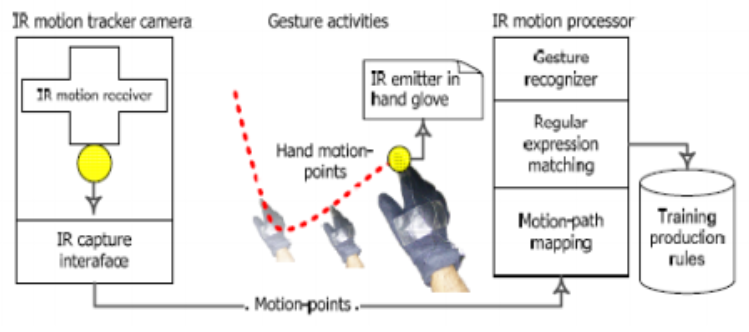
\includegraphics[width=0.4\textwidth]{img/Feedback-Mechanismen/Gestensteuerung.png}
	\caption{Gestensteuerung}
	\label{fig:feedbackGestensteuerung}
\end{figure}

Aufgrund dieser Anforderungen wurde folgender Ansatz gewählt: Das Erkennungssystem besteht aus einer Infrarot Kamera, einer Infrarot LED und einem Handschuh, wobei kein spezieller Datenhandschuh hierfür verwendet wird. Es wird lediglich die Infrarot LED am Handschuh befestigt. Wenn eine neue Geste gelernt werden soll, so aktiviert der User die Infrarot LED während er die Geste in den Raum zeichnet. Sodann wird die Geste vom System zerlegt, d.h. es werden vom Startpunkt aus jeweils die Richtungen, in die der User die Geste von Punkt zu Punkt zeichnet (in Summe sind es acht mögliche Richtungen) im IR motion processor gespeichert. Wenn nun eine gelernte Geste vom System erkannt wird, dann wird über einen sogenannten \glqq User Interaction Manager\grqq , der das Smart Home System per Web-Service über die erkannte Geste und die damit verbundene Aktion informiert und sodann führt das Smart Home die auszuführende Operation aus.

\begin{figure}[h!]
	\centering
	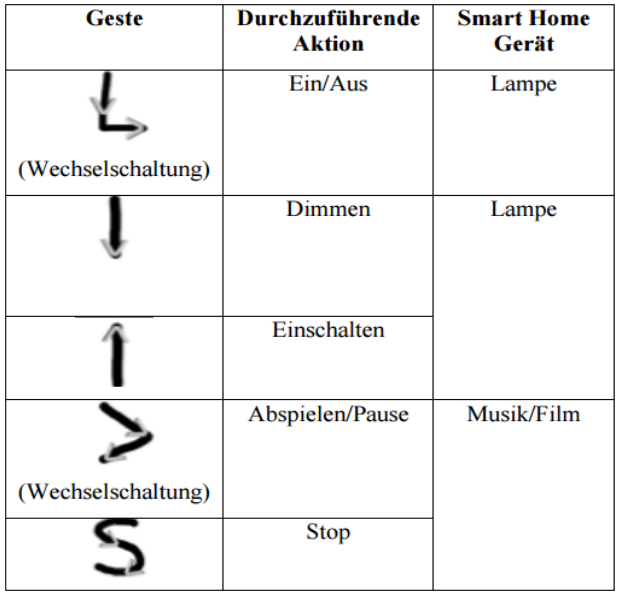
\includegraphics[width=0.4\textwidth]{img/Feedback-Mechanismen/Gestentabelle.png}
	\caption{Gestentabelle}
	\label{fig:feedbackGestentabelle}
\end{figure}

\subsection{Vergleich der Feedback-Mechanismen}

\begin{table}[H]
	\begin{tabularx}{\textwidth}{
			>{\hsize=1\hsize}X 
			>{\hsize=1\hsize}X
			>{\hsize=1\hsize}X
			% sum=2.0\hsize for 2 columns
		}
		\hline
		\textbf{System}	
		& \textbf{Kosten}
		& \textbf{Steuerung} \\
		\hline 
	 	Homey
		& 299,00 \$
		& Sprache \\
		\hline 
	 	IVEE
		& 200,00 €
		& Sprache \\	
		\hline 
	 	CastleOS Voice
		& 199,99 \$
		& Sprache \\
		\hline 
	 	Amazon Echo
		& 179,99 \$
		& Sprache \\
		\hline 
	 	EnBlink
		& 89,99 \$
		& Sprache \\
		\hline 
	 	Z-Wave.me
		& 74,00 €
		& Fernbedienung \\
		\hline 
	 	Düwi
		& 70,80 €
		& Fernbedienung \\
		\hline 
	 	Reemo
		& 299,00 €
		& Gestik \\
		\hline 
	 	OneCue
		& 129,00 \$
		& Gestik \\
		\hline 
	 	Kinect (das Gerät selbst)
		& 110,00 \$
		& Gestik \\
		\hline 
	\end{tabularx}
	\caption{Vergleichstabelle}
\end{table}

\subsection{Einsatzmöglichkeiten im Projekt}
Alle bisher aufgelistete Anwendungen können für Feedback im Projekt eingesetzt werden. Eine große Rolle spielen die Kosten, die im Vergleichsliste deutlich zu erkennen sind. Das Kostenfaktor variiert sich im Bereich von 200€, was für eine mögliche Testumsetzung sehr aufwändig wäre. Die Benutzbarkeit von den Systemen scheint überhaupt nicht schwierig zu sein, sondern sehr schnell erlernbar, effizient und anpassungsfähig. Die Anwendungen können von einzelnen sowie auch von mehreren Benutzern gesteuert werden. Als Vorteil bei Sprachsteuerungssystemen gilt das es keine vordefinierte Sätze gelernt werden sollen um die Hausgeräte zu steuern. Einfach angesprochene Sätze werden vom System verstanden und richtig ausgeführt.

Es wäre auch eine Möglichkeit das System selbst zu bauen und zu testen. Dazu sollen ein Kinect,
Bewegungssensor, Software für Spracherkennung, Schnittstelle, zusätzliche Kamera, Mikrofon
besorgt werden, damit das ganze aufbauen zu können entweder für Sprachsteuerung oder Gestensteuerung. Dabei entstehen Kosten für das ganze um es zu realisieren und wird auch eine
Menge Zeit kosten.

\subsection{HomeKit iOS Gerätesteuerung}
Die nachfolgenden Ausführungen beziehen sich auf die Onlinequellen \glqq A Home for Apple – HomeKit unter iOS 9\grqq\footnote{\url{https://www.apfellike.com/2015/10/a-home-for-apple-homekit-unter-ios-9/}}, \glqq Geräte über den Raspberry Pi und HomeKit steuern\grqq\footnote{\url{https://alexbloggt.com/geraete-ueber-den-raspberry-pi-und-homekit-steuern/}} und \glqq So wird dein Raspberry Pi mit Z-Wave zur Apple HomeKit Bridge\grqq\footnote{\url{http://www.siio.de/so-wird-dein-raspberry-pi-mit-z-wave-zur-apple-homekit-bridge/}}

Sprachsteuerung mit Hilfe von HomeKit, benötigt zusätzlich App (z.B. Eve) Installation auf dem iOS Gerät.

Das Apple HomeKit ist ein System die auch innerhalb des Smart Homes benutzt werden kann. Die
Komponenten des Hauses können über das Smartphone oder das Tablet gesteuert werden. Ab iOS 8
ist es möglich, das iPhone oder das Tablet dazu zu verwenden, Komponenten in der Wohnung zu
steuern. Dadurch wird beispielsweise ein Licht eingeschaltet, die Temperatur an einer Heizung
geändert oder ein Herd eingeschaltet. Bei Apple HomeKit sendet das Smartphone Befehle an ein Set Top Box, der dann diese an jeweilige Geräte im Haus überträgt.

Um HomeKit-Steuerung zu ermöglichen, muss das zu steuernde Gerät über einen HTTP-Request am Raspberry Pi zu steuern sein.

Für die Einbindung von Geräten empfiehlt es sich, erst einmal mit Geräten zu beginnen, welche eine Schalterfunktion haben, da dieses von HomeKit unterstützt werden. In den Einstellungen wird den Punkt \glqq Geräte\grqq{} ausgewählt. In der Gerätegruppe, wähle Z-Wave Gerätetyp aus.

Nach dem Klicken der Schaltfläche wird eine Übersicht mit 4 Schritten angezeigt. Überprüfe als
erstes, ob dein Gerät exkludiert ist (im alten Netzwerk gelöscht wurde) und tatsächlich bereit ist inkludiert zu werden. Falls nicht, führe einfach noch einmal eine Exklusion durch um sicher zu gehen, dass das Gerät inkludiert werden kann.

Wenn alles fertig ist, wird die Schaltfläche \glqq Anlernen starten\grqq{} gedrückt und wiederholt den Taster am Geräte gedrückt, um dieses zu inkludieren (mehr dazu siehe Handbuch des Z-Wave Gerätes). Nach einer kurzen Zeit sollte das Gerät gefunden werden. Die Oberfläche informiert, sobald das Gerät gefunden wurde und konfiguriert wird.

\begin{figure}[h!]
	\centering
	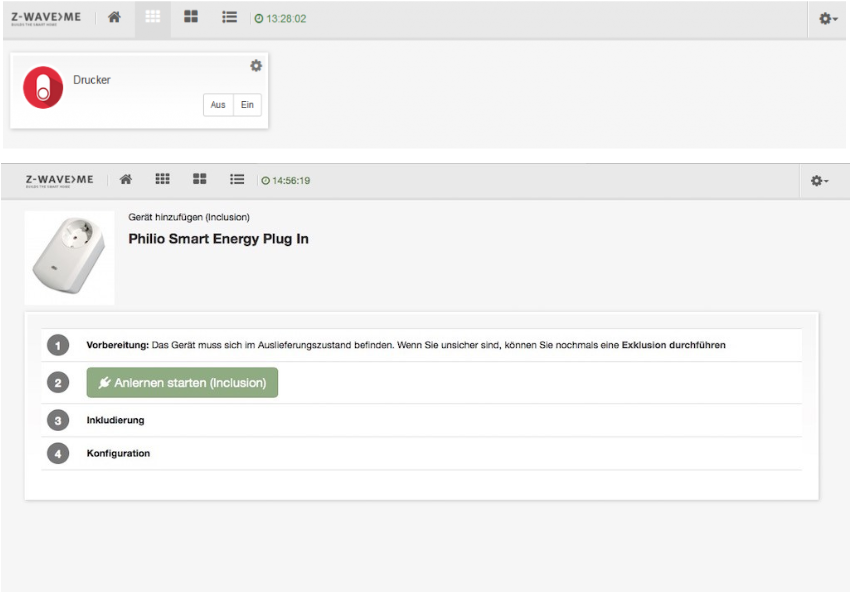
\includegraphics[width=0.7\textwidth]{img/Feedback-Mechanismen/HomeKit.png}
	\caption{HomeKit iOS}
	\label{fig:feedbackHomeKit}
\end{figure}

Um Z-Wave Geräte für HomeKit erkennbar zu machen bedarf es noch einer weiteren App, welche ebenfalls im App Store der Smart Home UI herunterladen und installieren werden kann.In die Einstellungen wird „Anwendungen“ ausgewählt. Die \glqq App Apple HomeKit Gate\grqq{} wird installiert, eine individuelle Name eingeben und entscheiden, wie Raspberry in der HomeKit App heißen soll. Da das Raspberry als Bridge für HomeKit dient, behalten alle inkludierten Geräte und erstellten Apps ihren Namen in dem HomeKit Apps bei. Nachdem die \glqq HomeKit Gate\grqq App installiert wurde, soll es auf Rapsberry Pi Konsole gewechselt werden und dort folgende Befehl ausgeführt werden:

\textbf{tail -f /var/log/z-way-server.log}

Dadurch werden diverse Informationen in der Konsole ausgegeben. Unter anderem auch der Punkt \glqq HomeKit PIN\grqq. Dieser PIN sollte wie so aussehen: XXXXXXXX

\begin{figure}[h!]
	\centering
	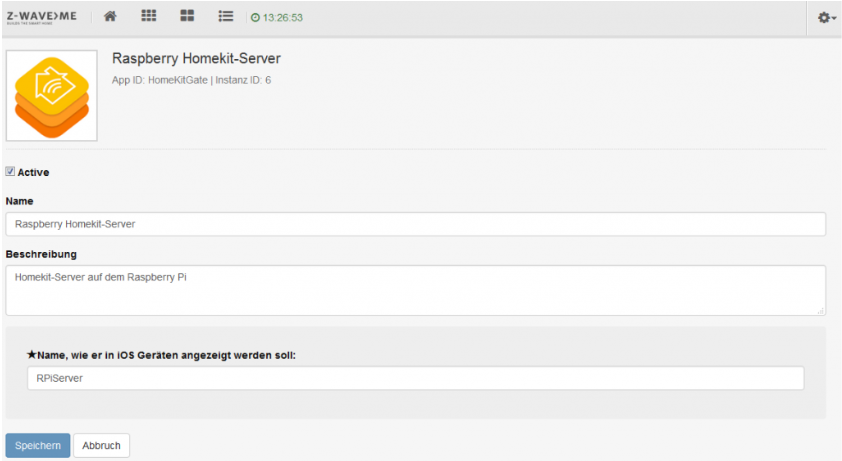
\includegraphics[width=0.7\textwidth]{img/Feedback-Mechanismen/HomeKitKonfiguration.png}
	\caption{HomeKit iOS - Konfiguration}
	\label{fig:feedbackHomeKitKonfiguration}
\end{figure}

Raspberry Pi ist nun ein vollständig konfiguriertes HomeKit Accessoire, welches in jeder HomeKit kompatiblen App verwendet werden kann. HomeKit-PIN soll eingegeben werden, sobald nach diesem gefragt wird und alle inkludierten Geräte werden unter der Raspberry HomeKit Bridge zu finden sein. Als App kann z.B. die \glqq MyTouchHome\grqq{} App verwendet werden, welche viele HomeKit-Funktionen bietet. Danach wird neu erstelltes Haus im APP ausgewählt. Da das Raspberry als Bridge dient, zählt es als Accessoire. Füge es entweder zu deinem Haus hinzu oder zu einem neu erstellten Raum und danach werden alle inkludierten Geräte angezeigt, sofern HomeKit den Gerätetyp unterstützt.

\begin{figure}[h!]
	\centering
	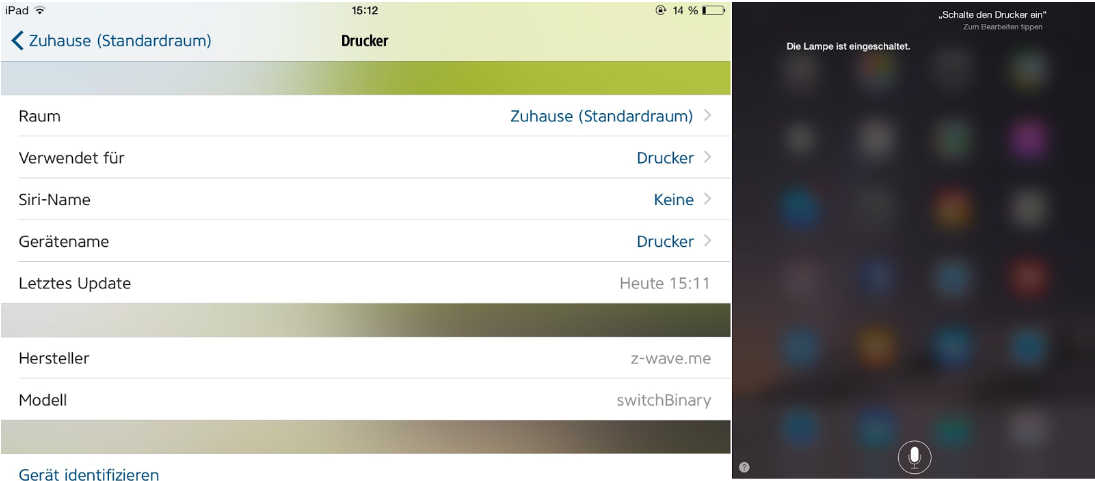
\includegraphics[width=0.7\textwidth]{img/Feedback-Mechanismen/HomeKitSteuerung.png}
	\caption{HomeKit iOS - Steuerung}
	\label{fig:feedbackHomeKitSteuerung}
\end{figure}

Mit Hilfe von RESTask Plugin innerhalb des Tasker Apps können die HTTP-Befehle für die
Steuerung von Geräten gesetzt werden. Ein Beispiel mit Fibaro HC (\url{http://www.siio.de/der-traum-vom-haus-per-sprachsteuerung-so-einfach/}).

\textbf{Material:}

\begin{itemize}
\item Android Smartphone oder Tablet (Android 4.4+ empfohlen)
\item Google Now
\item Tasker
\item RESTask Tasker Plugin
\item AutoVoice Tasker Plugin
\item Fibaro HC2
\end{itemize}

Google Now, Tasker, RESTask und AutoVoice werden installiert.
Beispiel: Die Raumbeleuchtung per Sprachbefehl ein und ausschalten. AutoVoice erwartet keinen exakten Satz, sondern jeder Aktion werden Schlüsselwörter oder Phrasen zugeordnet. Wenn der Befehl als \glqq Licht ein\grqq hinterlegt wird, funktioniert \glqq Ich möchte das LICHT EINschalten\grqq{} oder \glqq Bitte das LICHT EIN\grqq{} auch. Nicht funktionieren wird: \glqq Schalte die Lampe an\grqq{} oder \glqq Bitte das Zimmer beleuchten\grqq.

Als erstes AutoVoice auf Google Now konfigurieren. Dazu AutoVoice starten, \glqq Google Now
Integration\grqq{} auswählen und dann noch \glqq NOT ENABLED\grqq{} klicken. In der Bedienungshilfe AutoVoice auf \glqq An\grqq{} stellen. Die angezeigte Warnmeldung ist in Ordnung. Als nächstes aktivieren das \glqq OK Google\grqq{} Feature. Im Android Startmenü \glqq Google Einstellungen\grqq{} auswählen. Dort \glqq Suche \& Google
Now\grqq , dann \glqq Sprache\grqq{} anklicken. Ins Menü \glqq OK Google Erkennung\grqq{} und dort alles aktivieren und gegebenenfalls den Anweisungen folgen.

Tasker Beispiel: Bei \glqq Profile\grqq{} mit \glqq +\grqq{} und \glqq Ereignis\grqq{} auswählen. Weiter:

\begin{itemize}
\item Plugins -> AutoVoice -> \glqq Recognized\grqq{} auswählen
\item Stift oben Rechts -> Command Filter -> \glqq Licht ein\grqq{} hinterlegen
\item Via Haken oben rechts speichern -> in Tasker oben links zurück
\item \glqq Neuer Task\grqq{} poppt auf, wir klicken darauf und geben einen Namen ein (z.B. \glqq Licht ein\grqq)
\item Mit dem Plus in der Mitte einen Schritt hinzufügen
\item Plugins -> RESTask -> Stift oben rechts
\item Bei HOST wird die entsprechende API URL für \glqq Lampe Einschalten\grqq{} hinterlegt
\item Bei BasicAuth die Zugangsdaten der Fibaro HC2 hinterlegen (normal \glqq admin\grqq{} und \glqq admin\grqq)
\item Via Diskette oben Speicher -> in Tasker oben links zurück
\item Mit Play unten links kann \glqq Licht ein\grqq{} getestet werden
\item oben links zurück -> Tasker schließen
\end{itemize}

\newpage
\section{Personenidentifikation}
\subsection{Identifikation von Personen anhand des CO$_2$-Verbrauchs und Persona}
\emph{(von Alexander Keller)}

\subsubsection{Allgemein}
Das Thema im Modul "'Projekt Master"' lautet "`Mehrbenutzerbetrieb der Smart-Home-Technik mittels des Systems Z-Way"'. Ziel ist es, in einem Haushalt, welcher mittels verschiedener Komponenten von Smart-Home-Technik ausgestattet ist, kleine Kinder vor Gefahrenquellen zu sichern. Zu diesem Thema wurden bereits verschiedene Szenarien ausgearbeitet. Diese beschreiben Gefahrenquellen vor welchen Kleinkinder geschützt werden sollten, wenn sie sich allein im Raum aufhalten.

Ziel ist es, bei der Recherche zu ermitteln, wie viel CO$_2$ ein Mensch ausstößt und diesen anhand des Wertes in eine Persona zu unterteilen. Persona werden mithilfe von Merkmalen erstellt und diese einer Gruppe zugeordnet. Dabei wird häufig nicht nur eine Persona, sondern mehrere entworfen, so viele wie nötig sind, um die Benutzer des Systems abzudecken. Anschließend sollten aus diesen Personae jedoch die primären und sekundären Personae ausgewählt werden.

Im letzten Gruppengespräch wurde festgelegt, dass drei verschiedene Personae angenommen werden. Diese drei Personae unterscheiden sich in Geschlecht und Alter des Menschen. Diese Annahme widerspiegelt eine Familie, die aus einem Mann, eine Frau und zwei Kindern besteht. Mittels des CO$_2$ Sensors soll es möglich sein zu erkennen, ob sich eines der beiden Kinder im Raum aufhält. Nachdem erkannt wurde, ob sich eines der beiden Kindern alleine im Raum befindet, werden anschließend automatisiert per Smart-Home-Steuerung alle Gefahrenquellen abgeschaltet.

\subsubsection{Der Siegenia SensoAir CO$_2$-Sensor}
Der CO$_2$-Gehalt der Luft wird mit der Maßeinheit \gls{ppm}  mithilfe des Gerätes der Firma Siegenia gemessen. Der Sensor besitzt eine LED die je nach CO$_2$ Konzentration in der Luft in verschiedenen Farben aufleuchtet.

\begin{longtabu} to \linewidth {
		>{\hsize=1.0\hsize}X 
		>{\hsize=1.0\hsize}X
		% sum=2.0\hsize for 2 columns
	}
	% ----------- begin header -----------	
	\hline
	\textbf{LED Anzeige}					& \textbf{Auswirkung} \\
	\hline
	\endhead
	% ----------- end header -----------

	% ----------- begin footer -----------
	\multicolumn{2}{r}{{Fortsetzung auf nächster Seite}}  \\ 
	\endfoot
	\endlastfoot
	% ----------- end footer -----------
	blinkt 2x kurz rot (2500ppm)			& Luftqualität sehr schlecht \\
	\hline 
	blinkt 1x lang rot (ab 2000ppm)			& Luftqualität sehr schlecht \\
	\hline
	dauerhaft rot (1500ppm)					& Grenzwert für Büros und Klassenräume \\
	\hline
	gelb / rot (1000ppm)					& Grenzwert für Wohnräume \\
	\hline
	dauerhaft gelb (800 ppm)				& gefühlt schlecht Luft \\
	\hline
	grün / gelb (600 ppm)					& Luftqualität verschlechtert sich \\
	\hline
	dauerhaft grün (350 ppm)				& saubere Frischluft \\
	\hline	
	\caption{Statusanzeige des SensoAir}
\end{longtabu}

Um das Gerät der Firma Siegenia nutzen zu können, muss der Sensor kalibriert werden. Die Kalibrierung des Sensors dauert mindestens 30 Minuten und anschließend ist das Gerät betriebsbereit. In der Theorie sollte das Gerät erkennen wie viele Personen sich im Raum befinden und unterscheiden ob Kinder oder Erwachsener sich dort aufhalten. Um das zuordnen zu können, ist es notwendig zu evaluieren wie viel jede Person im Schnitt an CO$_2$ ausstößt.

\begin{figure}[h!]
	\centering
	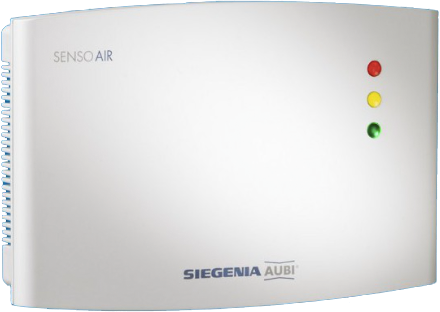
\includegraphics[width=0.4\textwidth]{img/PersonIdentification/sensoAir.png}
	\caption{Siegenia SensoAir (Tischgerät)}
	\label{fig:sensoAir}
\end{figure}

\subsubsection{Recherche zum CO$_2$-Ausstoß}
Der Stoffwechsel des Menschen ist dafür verantwortlich, dass der Mensch CO$_2$ freisetzt. Das ganze System ist sehr komplex, vielseitig und störanfällig. Alle Vorgänge der Nahrungsaufnahme, -verarbeitung und Ausscheidung von Restprodukten fallen darunter sowie die Atmung. Alle Lebewesen sind auf dieses System angewiesen um zu existieren. Die Bewegung, Ernährung und Atemluft beeinflussen den Ablauf des Stoffwechsels enorm und ist dadurch von Mensch zu Mensch völlig verschieden.

\subsubsection{Interview mit Dr. med. S. Blasko}
Zur Bearbeitung des Themas wurde Dr. med. S. Blaskos Hilfe beansprucht und ca. zwei Stunden über das Problem des CO$_2$-Ausstoßes beim Menschen gesprochen. Herr Blasko war zu Beginn von dem Thema Smart-Home-Technik sehr begeistert. Die Problemstellung wurde ihm ausführlich erklärt und gefragt, ob es denn möglich sei, mithilfe von CO$_2$-Werten zu unterscheiden, ob eine erwachsene Person sich in einem Raum befindet oder ein Kind.

Seine Antwort darauf war ein klares nein. Der Stoffwechsel jeder einzelnen Person ist so grundverschieden, dass man keinen festen Wert bzw. keine Konstante festlegen kann. 

Für ein Grundverständnis erklärte er, dass der Stoffwechsel konkret für
die Aufnahme, Transport und chemische Umwandlung von Nährstoffen im Körper zuständig ist, sowie die Abgabe von Stoffwechselendprodukten. Jeder Mensch hat einen anderen und individuellen Stoffwechsel, den man grob in drei Gruppen unterscheiden kann. Zum einen gibt es den "`Mesomorphen"' Stoffwechsel, der bei eher muskulösen Menschen vorkommt und welcher durchschnittlich ist. Bei Menschen die eher eine schmale Figur besitzen nennt man den Stoffwechsel "`Ektomorph"' und dieser ist sehr hoch. Bei der Persona "`Der runde Typ"' wo der Stoffwechsel sehr langsam ist spricht man von "`Endomorph"'. Anhand der drei Kategorien könnte man annehmen, dass man die verschiedenen Personen in diese Personas aufteilt und dort einen konstanten Wert festlegt. Doch diese Theorie wurde von Dr. med. S. Blasko dementiert, weil trotz der Unterscheidung es nicht eindeutig sei den CO$_2$ Gehalt einer bestimmten Persona zuzuordnen. Als Beispiel nannte er mehrere Usecases die es unmöglich machen, anhand eines Wertes die Person eindeutig zu identifizieren.

Wir nehmen an, das eine junge zierliche Frau entspannt auf dem Sofa liegt und deren Stoffwechsel in diesem Moment gerade gegen null geht. Im nächsten Moment kommt ein Kind vom Spielen nach Hause und betritt den Raum. Der CO$_2$ Ausstoß des Kindes ist in diesem Moment enorm groß und das Ergebnis wäre so sehr verfälscht, dass keine eindeutige Annahme getroffen werden kann, welche Persona sich im Raum befindet. Dazu kommen noch Fehlerquellen wie z.B. geöffnete Fenster
oder Räume enormer Größe.

Da das zu entwickelnde Modul ein sehr hohes Maß an Zuverlässigkeit mit sich
bringen sollte, ist die Annahme, die Persona via CO$_2$ zu bestimmen nicht aussagekräftig genug. Von Dr. med. S. Blasko kam ebenfalls der Vorschlag, dieses System anhand eines Türsensors umzusetzen. Dieser bestimmt die Größe der Person, um dann entscheiden zu können, ob es sich um ein Kind oder einen Erwachsenen handelt.

\subsubsection{Internetrecherche}
Eine Recherche im Internet lieferte schlussendlich das gleiche Ergebnis wie  Dr. med. S. Blasko ausführlich erklärte. Der Stoffwechsel eines jeden Menschen ist derart grundverschiedenen, dass es ist nicht möglich ist, mithilfe einer Konstante festzulegen welche Persona sich im Raum aufhält.

%TODO Quellen
%Webquellen
%[Pep 1]		Z-Wave Device Library
%http://www.pepper1.net/zwavedb/device/585
%[Zwa 1]		Z-Wave Erfahrungsbericht
%http://www.zwave-review.com/tests/Phlio_mutisensor.php
%[Zwa 2]		Problembehebung mit Philip Mehrfachsensor
%http://www.zwave.de/problembehebung-mit-philio-mehrfachsensor/
